\PassOptionsToPackage{unicode=true}{hyperref} % options for packages loaded elsewhere
\PassOptionsToPackage{hyphens}{url}
\PassOptionsToPackage{dvipsnames,svgnames*,x11names*}{xcolor}
%
\documentclass[]{krantz}
\usepackage{lmodern}
\usepackage{amssymb,amsmath}
\usepackage{ifxetex,ifluatex}
\usepackage{fixltx2e} % provides \textsubscript
\ifnum 0\ifxetex 1\fi\ifluatex 1\fi=0 % if pdftex
  \usepackage[T1]{fontenc}
  \usepackage[utf8]{inputenc}
  \usepackage{textcomp} % provides euro and other symbols
\else % if luatex or xelatex
  \usepackage{unicode-math}
  \defaultfontfeatures{Ligatures=TeX,Scale=MatchLowercase}
\fi
% use upquote if available, for straight quotes in verbatim environments
\IfFileExists{upquote.sty}{\usepackage{upquote}}{}
% use microtype if available
\IfFileExists{microtype.sty}{%
\usepackage[]{microtype}
\UseMicrotypeSet[protrusion]{basicmath} % disable protrusion for tt fonts
}{}
\IfFileExists{parskip.sty}{%
\usepackage{parskip}
}{% else
\setlength{\parindent}{0pt}
\setlength{\parskip}{6pt plus 2pt minus 1pt}
}
\usepackage{xcolor}
\usepackage{hyperref}
\hypersetup{
            pdftitle={Phân tích dữ liệu thực tế với R},
            pdfauthor={Hoàng Đức Anh},
            colorlinks=true,
            linkcolor=Maroon,
            citecolor=Blue,
            urlcolor=Blue,
            breaklinks=true}
\urlstyle{same}  % don't use monospace font for urls
\usepackage{color}
\usepackage{fancyvrb}
\newcommand{\VerbBar}{|}
\newcommand{\VERB}{\Verb[commandchars=\\\{\}]}
\DefineVerbatimEnvironment{Highlighting}{Verbatim}{commandchars=\\\{\}}
% Add ',fontsize=\small' for more characters per line
\usepackage{framed}
\definecolor{shadecolor}{RGB}{248,248,248}
\newenvironment{Shaded}{\begin{snugshade}}{\end{snugshade}}
\newcommand{\AlertTok}[1]{\textcolor[rgb]{0.33,0.33,0.33}{#1}}
\newcommand{\AnnotationTok}[1]{\textcolor[rgb]{0.37,0.37,0.37}{\textbf{\textit{#1}}}}
\newcommand{\AttributeTok}[1]{\textcolor[rgb]{0.61,0.61,0.61}{#1}}
\newcommand{\BaseNTok}[1]{\textcolor[rgb]{0.06,0.06,0.06}{#1}}
\newcommand{\BuiltInTok}[1]{#1}
\newcommand{\CharTok}[1]{\textcolor[rgb]{0.5,0.5,0.5}{#1}}
\newcommand{\CommentTok}[1]{\textcolor[rgb]{0.37,0.37,0.37}{\textit{#1}}}
\newcommand{\CommentVarTok}[1]{\textcolor[rgb]{0.37,0.37,0.37}{\textbf{\textit{#1}}}}
\newcommand{\ConstantTok}[1]{\textcolor[rgb]{0,0,0}{#1}}
\newcommand{\ControlFlowTok}[1]{\textcolor[rgb]{0.27,0.27,0.27}{\textbf{#1}}}
\newcommand{\DataTypeTok}[1]{\textcolor[rgb]{0.27,0.27,0.27}{#1}}
\newcommand{\DecValTok}[1]{\textcolor[rgb]{0.06,0.06,0.06}{#1}}
\newcommand{\DocumentationTok}[1]{\textcolor[rgb]{0.37,0.37,0.37}{\textbf{\textit{#1}}}}
\newcommand{\ErrorTok}[1]{\textcolor[rgb]{0.14,0.14,0.14}{\textbf{#1}}}
\newcommand{\ExtensionTok}[1]{#1}
\newcommand{\FloatTok}[1]{\textcolor[rgb]{0.06,0.06,0.06}{#1}}
\newcommand{\FunctionTok}[1]{\textcolor[rgb]{0,0,0}{#1}}
\newcommand{\ImportTok}[1]{#1}
\newcommand{\InformationTok}[1]{\textcolor[rgb]{0.37,0.37,0.37}{\textbf{\textit{#1}}}}
\newcommand{\KeywordTok}[1]{\textcolor[rgb]{0.27,0.27,0.27}{\textbf{#1}}}
\newcommand{\NormalTok}[1]{#1}
\newcommand{\OperatorTok}[1]{\textcolor[rgb]{0.43,0.43,0.43}{\textbf{#1}}}
\newcommand{\OtherTok}[1]{\textcolor[rgb]{0.37,0.37,0.37}{#1}}
\newcommand{\PreprocessorTok}[1]{\textcolor[rgb]{0.37,0.37,0.37}{\textit{#1}}}
\newcommand{\RegionMarkerTok}[1]{#1}
\newcommand{\SpecialCharTok}[1]{\textcolor[rgb]{0,0,0}{#1}}
\newcommand{\SpecialStringTok}[1]{\textcolor[rgb]{0.5,0.5,0.5}{#1}}
\newcommand{\StringTok}[1]{\textcolor[rgb]{0.5,0.5,0.5}{#1}}
\newcommand{\VariableTok}[1]{\textcolor[rgb]{0,0,0}{#1}}
\newcommand{\VerbatimStringTok}[1]{\textcolor[rgb]{0.5,0.5,0.5}{#1}}
\newcommand{\WarningTok}[1]{\textcolor[rgb]{0.37,0.37,0.37}{\textbf{\textit{#1}}}}
\usepackage{longtable,booktabs}
% Fix footnotes in tables (requires footnote package)
\IfFileExists{footnote.sty}{\usepackage{footnote}\makesavenoteenv{longtable}}{}
\usepackage{graphicx,grffile}
\makeatletter
\def\maxwidth{\ifdim\Gin@nat@width>\linewidth\linewidth\else\Gin@nat@width\fi}
\def\maxheight{\ifdim\Gin@nat@height>\textheight\textheight\else\Gin@nat@height\fi}
\makeatother
% Scale images if necessary, so that they will not overflow the page
% margins by default, and it is still possible to overwrite the defaults
% using explicit options in \includegraphics[width, height, ...]{}
\setkeys{Gin}{width=\maxwidth,height=\maxheight,keepaspectratio}
\setlength{\emergencystretch}{3em}  % prevent overfull lines
\providecommand{\tightlist}{%
  \setlength{\itemsep}{0pt}\setlength{\parskip}{0pt}}
\setcounter{secnumdepth}{5}
% Redefines (sub)paragraphs to behave more like sections
\ifx\paragraph\undefined\else
\let\oldparagraph\paragraph
\renewcommand{\paragraph}[1]{\oldparagraph{#1}\mbox{}}
\fi
\ifx\subparagraph\undefined\else
\let\oldsubparagraph\subparagraph
\renewcommand{\subparagraph}[1]{\oldsubparagraph{#1}\mbox{}}
\fi

% set default figure placement to htbp
\makeatletter
\def\fps@figure{htbp}
\makeatother

\usepackage{booktabs}
\usepackage{longtable}
\usepackage[bf,singlelinecheck=off]{caption}

\usepackage{framed,color}
\definecolor{shadecolor}{RGB}{248,248,248}

\renewcommand{\textfraction}{0.05}
\renewcommand{\topfraction}{0.8}
\renewcommand{\bottomfraction}{0.8}
\renewcommand{\floatpagefraction}{0.75}

\renewenvironment{quote}{\begin{VF}}{\end{VF}}
\let\oldhref\href
\renewcommand{\href}[2]{#2\footnote{\url{#1}}}

\makeatletter
\newenvironment{kframe}{%
\medskip{}
\setlength{\fboxsep}{.8em}
 \def\at@end@of@kframe{}%
 \ifinner\ifhmode%
  \def\at@end@of@kframe{\end{minipage}}%
  \begin{minipage}{\columnwidth}%
 \fi\fi%
 \def\FrameCommand##1{\hskip\@totalleftmargin \hskip-\fboxsep
 \colorbox{shadecolor}{##1}\hskip-\fboxsep
     % There is no \\@totalrightmargin, so:
     \hskip-\linewidth \hskip-\@totalleftmargin \hskip\columnwidth}%
 \MakeFramed {\advance\hsize-\width
   \@totalleftmargin\z@ \linewidth\hsize
   \@setminipage}}%
 {\par\unskip\endMakeFramed%
 \at@end@of@kframe}
\makeatother

\renewenvironment{Shaded}{\begin{kframe}}{\end{kframe}}

\usepackage{makeidx}
\makeindex

\urlstyle{tt}

\usepackage{amsthm}
\makeatletter
\def\thm@space@setup{%
  \thm@preskip=8pt plus 2pt minus 4pt
  \thm@postskip=\thm@preskip
}
\makeatother

\frontmatter

%%%%%%%%%%%%%%%%%%%%%%%%%%%%%%%%%%%%%%%%%%%%%%%%%%
% New translation of phrases into Vietnamese
%%%%%%%%%%%%%%%%%%%%%%%%%%%%%%%%%%%%%%%%%%%%%%%%%%

\usepackage{booktabs}
\usepackage{longtable}
\usepackage[utf8]{inputenc}
\usepackage[vietnamese]{babel}
\addto\captionsvietnamese{%
  \renewcommand{\listfigurename}%
    {Danh mục biểu đồ}%
  \renewcommand{\listtablename}%
    {Danh mục bảng}%
}

%%%%%%%%%%%%%%%%%%%%%%%%%%%%%%%%%%%%%%%%%%%%%%%%%
% Highlighting R codes

\usepackage{listings}
\usepackage{color}
\usepackage{fancyvrb}
\renewcommand{\VerbBar}{|}
\renewcommand{\VERB}{\Verb[commandchars=\\\{\}]}
\DefineVerbatimEnvironment{Highlighting}{Verbatim}{commandchars=\\\{\}}
% Add ',fontsize=\small' for more characters per line
\usepackage{framed}
\definecolor{shadecolor}{RGB}{248,248,248}
\renewenvironment{Shaded}{\begin{snugshade}}{\end{snugshade}}
\renewcommand{\AlertTok}[1]{\textcolor[rgb]{0.94,0.16,0.16}{#1}}
\renewcommand{\AnnotationTok}[1]{\textcolor[rgb]{0.56,0.35,0.01}{\textbf{\textit{#1}}}}
\renewcommand{\AttributeTok}[1]{\textcolor[rgb]{0.77,0.63,0.00}{#1}}
\renewcommand{\BaseNTok}[1]{\textcolor[rgb]{0.00,0.00,0.81}{#1}}
\renewcommand{\BuiltInTok}[1]{#1}
\renewcommand{\CharTok}[1]{\textcolor[rgb]{0.31,0.60,0.02}{#1}}
\renewcommand{\CommentTok}[1]{\textcolor[rgb]{0.56,0.35,0.01}{\textit{#1}}}
\renewcommand{\CommentVarTok}[1]{\textcolor[rgb]{0.56,0.35,0.01}{\textbf{\textit{#1}}}}
\renewcommand{\ConstantTok}[1]{\textcolor[rgb]{0.00,0.00,0.00}{#1}}
\renewcommand{\ControlFlowTok}[1]{\textcolor[rgb]{0.13,0.29,0.53}{\textbf{#1}}}
\renewcommand{\DataTypeTok}[1]{\textcolor[rgb]{0.13,0.29,0.53}{#1}}
\renewcommand{\DecValTok}[1]{\textcolor[rgb]{0.00,0.00,0.81}{#1}}
\renewcommand{\DocumentationTok}[1]{\textcolor[rgb]{0.56,0.35,0.01}{\textbf{\textit{#1}}}}
\renewcommand{\ErrorTok}[1]{\textcolor[rgb]{0.64,0.00,0.00}{\textbf{#1}}}
\renewcommand{\ExtensionTok}[1]{#1}
\renewcommand{\FloatTok}[1]{\textcolor[rgb]{0.00,0.00,0.81}{#1}}
\renewcommand{\FunctionTok}[1]{\textcolor[rgb]{0.00,0.00,0.00}{#1}}
\renewcommand{\ImportTok}[1]{#1}
\renewcommand{\InformationTok}[1]{\textcolor[rgb]{0.56,0.35,0.01}{\textbf{\textit{#1}}}}
\renewcommand{\KeywordTok}[1]{\textcolor[rgb]{0.13,0.29,0.53}{\textbf{#1}}}
\renewcommand{\NormalTok}[1]{#1}
\renewcommand{\OperatorTok}[1]{\textcolor[rgb]{0.81,0.36,0.00}{\textbf{#1}}}
\renewcommand{\OtherTok}[1]{\textcolor[rgb]{0.56,0.35,0.01}{#1}}
\renewcommand{\PreprocessorTok}[1]{\textcolor[rgb]{0.56,0.35,0.01}{\textit{#1}}}
\renewcommand{\RegionMarkerTok}[1]{#1}
\renewcommand{\SpecialCharTok}[1]{\textcolor[rgb]{0.00,0.00,0.00}{#1}}
\renewcommand{\SpecialStringTok}[1]{\textcolor[rgb]{0.31,0.60,0.02}{#1}}
\renewcommand{\StringTok}[1]{\textcolor[rgb]{0.31,0.60,0.02}{#1}}
\renewcommand{\VariableTok}[1]{\textcolor[rgb]{0.00,0.00,0.00}{#1}}
\renewcommand{\VerbatimStringTok}[1]{\textcolor[rgb]{0.31,0.60,0.02}{#1}}
\renewcommand{\WarningTok}[1]{\textcolor[rgb]{0.56,0.35,0.01}{\textbf{\textit{#1}}}}

%%%%%%%%%%%%%%%%%%%%%%%%%%%%%%%%%%%%%%%%%%%%
% Lines in heading
\usepackage[]{natbib}
\bibliographystyle{apalike}

\title{Phân tích dữ liệu thực tế với R}
\author{Hoàng Đức Anh}
\date{2018-09-23}

\usepackage{amsthm}
\newtheorem{theorem}{Định lý}[chapter]
\newtheorem{lemma}{Lemma}[chapter]
\newtheorem{corollary}{Corollary}[chapter]
\newtheorem{proposition}{Proposition}[chapter]
\newtheorem{conjecture}{Conjecture}[chapter]
\theoremstyle{definition}
\newtheorem{definition}{Definition}[chapter]
\theoremstyle{definition}
\newtheorem{example}{Example}[chapter]
\theoremstyle{definition}
\newtheorem{exercise}{Bài tập}[chapter]
\theoremstyle{remark}
\newtheorem*{remark}{Remark}
\newtheorem*{solution}{Đáp án}
\let\BeginKnitrBlock\begin \let\EndKnitrBlock\end
\begin{document}
\maketitle

% you may need to leave a few empty pages before the dedication page

%\cleardoublepage\newpage\thispagestyle{empty}\null
%\cleardoublepage\newpage\thispagestyle{empty}\null
%\cleardoublepage\newpage
\thispagestyle{empty}

\begin{center}
Gửi con trai,

%\includegraphics{images/dedication.pdf}
nếu không có con, hai năm trước bố đã có thể hoàn thành cuốn sách này!
\end{center}

\setlength{\abovedisplayskip}{-5pt}
\setlength{\abovedisplayshortskip}{-5pt}

{
\hypersetup{linkcolor=}
\setcounter{tocdepth}{2}
\tableofcontents
}
\listoftables
\listoffigures
\hypertarget{li-m-u}{%
\chapter*{Lời mở đầu}\label{li-m-u}}


Trong quá trình triển khai công việc thực tế tại nhiều tổ chức khác
nhau, tôi nhận thấy một hiện thực là mặt bằng kiến thức thực tế về phân
tích dữ liệu trên thị trường Việt Nam còn rất yếu. Phần lớn, các bạn làm
trong ngành phân tích dữ liệu rơi vào một trong hai nhóm sau:

\begin{itemize}
\item
  Nhóm một, \textbf{chưa có nền tảng về phân tích thống kê}. Ở nhóm này,
  các bạn thường không được đào tạo bài bản hoặc không có đủ điều kiện
  (phần lớn là về thời gian) để học các kiến thức về phân tích thống kê.
  Do nhu cầu của công việc, các bạn có thành thạo các kỹ năng về xây
  dựng báo cáo và phân tích khám phá dữ liệu đơn giản với SQL và Excel.
  Các bạn này thường thuộc các nhóm phân tích báo cáo (Business
  Intelligence) tại các tổ chức lớn hoặc làm trong startup. Điểm mạnh
  của nhóm này là làm việc sát với các bộ phận kinh doanh, hiểu rõ
  nghiệp vụ và nhu cầu nghiệp vụ. Tuy nhiên, điểm yếu của các bạn lại là
  không thể ứng dụng hoặc tự học và không biết cách triển khai các ứng
  dụng của khoa học dữ liệu ở mức độ cao vào công việc thực tế.
\item
  Nhóm hai, \textbf{có nền tảng vững vàng về kiến thức thống kê, dự báo
  nhưng lại quá chú trọng vào các yếu tố kỹ thuật}. Ở nhóm này, các bạn
  đều có nền tảng kiến thức về toán, thống kê rất tốt. Một số bạn được
  học và đào tạo cơ bản về khoa học dữ liệu, học máy và các ứng dụng của
  khoa học dữ liệu. Các bạn này có thiên hướng thích xây dựng mô hình dự
  báo, thích làm các bài toán lớn trong kinh doanh. Điểm mạnh của nhóm
  này là rất thông minh, chịu khó học hỏi và có thể áp dụng những kỹ
  thuật phân tích mới vào thực tế một cách nhanh chóng. Nhưng ngược lại,
  nhóm này lại có nhược điểm chết người là có thói quen chỉ tập trung
  vào việc phân tích dữ liệu mà thiếu đi cái nhìn tổng quát trong việc
  giải quyết bài toán thực tế. Không chỉ thế, nhóm này không có thế mạnh
  trong việc trình bày và giao tiếp, dẫn đến các kết quả thực tế không
  được các đơn vị kinh doanh nghiệp vụ đón nhận và sử dụng.
\end{itemize}

Đối với một tổ chức muốn phát triển dựa vào dữ liệu và muốn biến các
quyết định của tổ chức dựa vào phân tích dữ liệu, cả hai nhóm trên đều
là các trạng thái nên tránh và phải cân bằng được cả hai. Cuốn sách này
sẽ phân tích và giúp các bạn làm trong lĩnh vực phân tích dữ liệu hiểu
rõ hơn các ưu nhược điểm của chính mình.

\hypertarget{tai-sao-nen-oc-cun-sach-nay}{%
\section*{Tại sao nên đọc cuốn sách
này}\label{tai-sao-nen-oc-cun-sach-nay}}


Việc viết cuốn sách này xuất phát thuần túy từ nhu cầu cá nhân của tác
giả. Trong quá trình làm việc thực tế, bản thân tác giả luôn có mong
muốn tổng hợp và đúc rút các kiến thức phân tích thực tế. Tuy nhiên, khi
bắt đầu bắt tay vào xây dựng cuốn sách, tác giả cũng có mong muốn có thể
đúc kết và giúp cho các tổ chức, bộ phận muốn tập trung vào và khai thác
sức mạnh của phân tích dữ liệu trong thực tế có thể có thêm các nguồn
tài liệu và kinh nghiệm, vốn rất ít được chia sẻ thực tế, để có thể
thành công hơn trong công việc triển khai.

Thêm vào đó, trong quá trình làm việc và giảng dạy cho các học viên, tác
giả luôn nhận được câu hỏi: \emph{Thưa thày, em không được đào tạo bài
bản về phân tích thống kê cũng như khoa học dữ liệu, liệu em có thể trở
thành chuyên gia phân tích dữ liệu được không?}

Tác giả luôn trăn trở với câu hỏi trên cũng như với kinh nghiệm đào tạo
thực tế và xây dựng năng lực phân tích dữ liệu ở VPBank, quyển sách này
được viết ra theo cách tiếp cận \emph{ứng dụng} của khoa học dữ liệu
trong hoạt động kinh doanh. Do đó, ngôn ngữ cũng như cách tiếp cận trong
cuốn sách này được cố gắng viết một cách đơn giản, dễ hiểu để trình bày
các kiến thức, thuật ngữ khó hiểu của khoa học dữ liệu thành các ngôn
ngữ bình dân phù hợp với nhiều đối tượng.

Cuốn sách này sẽ không đi sâu vào lý thuyết của các thuật toán, mô hình
thống kê mà sẽ cố gắng trả lời các khía cạnh sau.

\begin{itemize}
\tightlist
\item
  Thuật toán, mô hình đó là gì?
\item
  Mô hình đó được sử dụng như thế nào?
\item
  Khi giải thích cho các đơn vị kinh doanh, ta cần phải giải thích điều
  gì?
\item
  Ứng dụng của mô hình trong thực tế
\end{itemize}

\hypertarget{cu-truc-cua-sach}{%
\section*{Cấu trúc của sách}\label{cu-truc-cua-sach}}


Cuốn sách được chia làm 3 phần theo thứ tự từ dễ đến khó, bao gồm.

\begin{itemize}
\tightlist
\item
  Phần một, các kiến thức cơ bản
\item
  Phần hai, các ứng dụng nâng cao
\item
  Phần ba, các vấn đề khác.
\end{itemize}

Chapters \ref{introduction} introduces a new topic, and \ldots{}

\hypertarget{cac-phn-mm-uc-s-dung}{%
\section*{Các phần mềm được sử dụng}\label{cac-phn-mm-uc-s-dung}}


I used the \textbf{knitr}\index{knitr} package \citep{xie2015} and the
\textbf{bookdown}\index{bookdown} package \citep{R-bookdown} to compile
my book. My R session information is shown below:

\begin{Shaded}
\begin{Highlighting}[]
\NormalTok{xfun}\OperatorTok{::}\KeywordTok{session_info}\NormalTok{()}
\end{Highlighting}
\end{Shaded}

\begin{verbatim}
## R version 3.4.0 (2017-04-21)
## Platform: x86_64-w64-mingw32/x64 (64-bit)
## Running under: Windows 10 x64 (build 17134)
## 
## Locale:
##   LC_COLLATE=English_United States.1252 
##   LC_CTYPE=English_United States.1252   
##   LC_MONETARY=English_United States.1252
##   LC_NUMERIC=C                          
##   LC_TIME=English_United States.1252    
## 
## Package version:
##   assertthat_0.2.0   backports_1.1.2   
##   base64enc_0.1.3    BH_1.66.0.1       
##   bindr_0.1.1        bindrcpp_0.2      
##   bookdown_0.7.18    cli_1.0.0         
##   colorspace_1.3-0   compiler_3.4.0    
##   crayon_1.3.4       dichromat_2.0.0   
##   digest_0.6.16      dplyr_0.7.4       
##   evaluate_0.11      ggplot2_3.0.0     
##   ggthemes_3.0.1     glue_1.3.0        
##   graphics_3.4.0     grDevices_3.4.0   
##   grid_3.4.0         gtable_0.2.0      
##   highr_0.7          htmltools_0.3.6   
##   jsonlite_1.5       knitr_1.20        
##   labeling_0.3       lattice_0.20.35   
##   lazyeval_0.2.0     magrittr_1.5      
##   markdown_0.8       MASS_7.3.47       
##   Matrix_1.2.9       methods_3.4.0     
##   mgcv_1.8.17        mime_0.5          
##   munsell_0.4.3      nlme_3.1.131      
##   pillar_1.2.1       pkgconfig_2.0.1   
##   plogr_0.2.0        plyr_1.8.4        
##   R6_2.2.2           RColorBrewer_1.1.2
##   Rcpp_0.12.18       reshape2_1.4.2    
##   rlang_0.2.1        rmarkdown_1.10    
##   rprojroot_1.3-2    rstudioapi_0.7    
##   scales_0.5.0       stats_3.4.0       
##   stringi_1.1.7      stringr_1.3.1     
##   tibble_1.4.2       tinytex_0.8       
##   tools_3.4.0        utf8_1.1.3        
##   utils_3.4.0        viridisLite_0.3.0 
##   withr_2.1.2        xfun_0.3          
##   yaml_2.2.0
\end{verbatim}

Package names are in bold text (e.g., \textbf{rmarkdown}), and inline
code and filenames are formatted in a typewriter font (e.g.,
\texttt{knitr::knit(\textquotesingle{}foo.Rmd\textquotesingle{})}).
Function names are followed by parentheses (e.g.,
\texttt{bookdown::render\_book()}).

\hypertarget{li-cam-on}{%
\section*{Lời cảm ơn}\label{li-cam-on}}


Cảm ơn những người sau đã giúp chúng tôi hoàn thành quyển sách

\BeginKnitrBlock{flushright}
Frida Gomam\\
on the Mars
\EndKnitrBlock{flushright}

\hypertarget{v-tac-gia}{%
\chapter*{Về tác giả}\label{v-tac-gia}}


Tác giả Hoàng Đức Anh hiên đang là trưởng phòng phân tích nâng cao của
ngân hàng \texttt{VPBank}. Đức Anh được đào tạo về phân tích dữ liệu tại
trường đại học kinh tế Vác-sa-va (Warsaw School of Economics),
Vác-sa-va, cộng hòa Ba Lan ở cả hai cấp, đại học và thạc sỹ từ năm
2009-2014.

\mainmatter

\hypertarget{part-cac-kin-thc-co-ban}{%
\part{Các kiến thức cơ bản}\label{part-cac-kin-thc-co-ban}}

\hypertarget{intro}{%
\chapter{Khoa học dữ liệu và nghề phân tích dữ liệu}\label{intro}}

\hypertarget{khoa-hoc-d-liu}{%
\section{Khoa học dữ liệu}\label{khoa-hoc-d-liu}}

\BeginKnitrBlock{theorem}[Pytago]
\protect\hypertarget{thm:unnamed-chunk-3}{}{\label{thm:unnamed-chunk-3}
\iffalse (Pytago) \fi{} }Trong một tam giác vuông, bình phương cạnh
huyền bằng tổng bình phương hai cạnh góc vuông

\[a^2 + b^2 = c^2\]
\EndKnitrBlock{theorem}

\hypertarget{tai-sao-phan-tich-d-liu-la-ngh-kho}{%
\section{Tại sao phân tích dữ liệu là nghề
khó?}\label{tai-sao-phan-tich-d-liu-la-ngh-kho}}

Phân tích dữ liệu đòi hỏi cùng lúc thực hiện ba nhóm công việc sau:

\begin{itemize}
\tightlist
\item
  Hiểu biết về vấn đề kinh doanh. Nghe có vẻ đơn giản nhưng qua quá
  trình làm việc thực tế, kinh nghiệm của tác giả cho thấy đây có lẽ là
  phần dễ bị bỏ qua nhất bỏi lẽ mấy nguyên nhân sau.

  \begin{itemize}
  \tightlist
  \item
    Sự khác biệt của vận hành kinh doanh so với hoạt động phân tích dữ
    liệu.
  \item
    Tư duy và thái độ của nhóm phân tích dữ liệu. Các bạn phân tích kinh
    doanh (hoặc đôi khi được gọi là phân tích kinh doanh) thường tự coi
    mình là đơn vị hỗ trợ và \emph{cung cấp} dữ liệu theo yêu cầu. Với
    lối tư duy thụ động này, các bạn sẽ không có nhu cầu tìm hiểu cặn kẽ
    các hoạt động kinh doanh, dẫn đến không hiểu hoạt động kinh doanh đủ
    sâu để có thể tư vấn và thuyết phục các bên kinh doanh trong việc
    triển khai các dự án phân tích dữ liệu mới.
  \item
    Nghiệp vụ kinh doanh rất phức tạp và thiếu hệ thống tài liệu ghi
    chép dưới góc độ khái quát cho hoạt động phân tích dữ liệu. Đây là
    vấn đề phần lớn các nhóm phân tích dữ liệu gặp phải. Để giải quyết
    vấn đề này, trong phần sau tác giả sẽ đưa ra phương pháp tìm hiểu
    hoạt động kinh doanh theo 6 nhóm vấn đề.
  \end{itemize}
\item
  Khai thác và phân tích dữ liệu
\item
  Trình bày, thuyết phục và tư vấn cho các bên kinh doanh về kết quả
  phân tích dữ liệu.
\end{itemize}

\textbf{Ba cấp độ của viết code}: Khi sử dụng các công cụ phân tích dữ
liệu (viết code), ta sẽ trải qua 3 cấp độ như sau:

\begin{enumerate}
\def\labelenumi{\arabic{enumi}.}
\tightlist
\item
  Viết thứ đơn giản. Ở cấp độ này, các bạn thường mới nhập môn phân tích
  dữ liệu, đầy lo lắng và thiếu tự tin ở bản thân và bắt đầu với những
  bài phân tích đơn giản để áp dụng các kiến thức mới học.
\item
  Viết càng nguy hiểm càng tốt. Ở giai đoạn này, các bạn đã có một lượng
  kiến thức nền tương đối vững và bắt đầu đi vào các phương pháp nâng
  cao. Do đó, các bạn thường có xu hướng khiến mọi thứ trở nên
  \emph{nguy hiểm}, tô vẽ và đưa ra nhiều yếu tố không thực sự cần
  thiết. Với các bạn có xu hướng trực quan hóa, sẽ là đưa ra các biểu đồ
  đầy màu sắc và cực kỳ nguy hiểm. Với các bạn có xu hướng xây dựng mô
  hình dự báo, sẽ là dùng mô hình dự báo, học máy hoặc deep-learning mọi
  lúc, mọi nơi. Kết quả sẽ khiến người đọc ấn tượng nhưng có thể chưa
  thực sự có tính ứng dụng cao.
\item
  Chỉ viết những thứ có khả năng tái sử dụng, giải quyết vấn đề bằng
  phương pháp đơn giản nhất có thể có. Ở giai đoạn này, các bạn đã dung
  hòa được rất nhiều kiến thức của nghành phân tích dữ liệu với nhau và
  tiếp cận các vấn đề một cách mạch lạc, logic và rất chặt chẽ. Các bạn
  nắm rất vững khi nào nên dùng các phương pháp phân tích khám phá dữ
  liệu đơn giản thay cho các thuật toán phức tạp trong việc giải quyết
  các vấn đề kinh doanh.
\end{enumerate}

\BeginKnitrBlock{theorem}[Pytago]
\protect\hypertarget{thm:unnamed-chunk-4}{}{\label{thm:unnamed-chunk-4}
\iffalse (Pytago) \fi{} }Trong một tam giác vuông, bình phương cạnh
huyền bằng tổng bình phương hai cạnh góc vuông

\[a^2 + b^2 = c^2\]
\EndKnitrBlock{theorem}

Figures and tables with captions will be placed in \texttt{figure} and
\texttt{table} environments, respectively.

\begin{Shaded}
\begin{Highlighting}[]
\KeywordTok{library}\NormalTok{(tidyverse)}
\NormalTok{iris }\OperatorTok\StringTok{ }
\StringTok{  }\KeywordTok{ggplot}\NormalTok{(}\KeywordTok{aes}\NormalTok{(Species, Sepal.Length)) }\OperatorTok{+}
\StringTok{  }\KeywordTok{geom_boxplot}\NormalTok{(}\KeywordTok{aes}\NormalTok{(}\DataTypeTok{fill =}\NormalTok{ Species)) }\OperatorTok{+}
\StringTok{  }\KeywordTok{theme_minimal}\NormalTok{()}
\end{Highlighting}
\end{Shaded}

\begin{figure}

{\centering 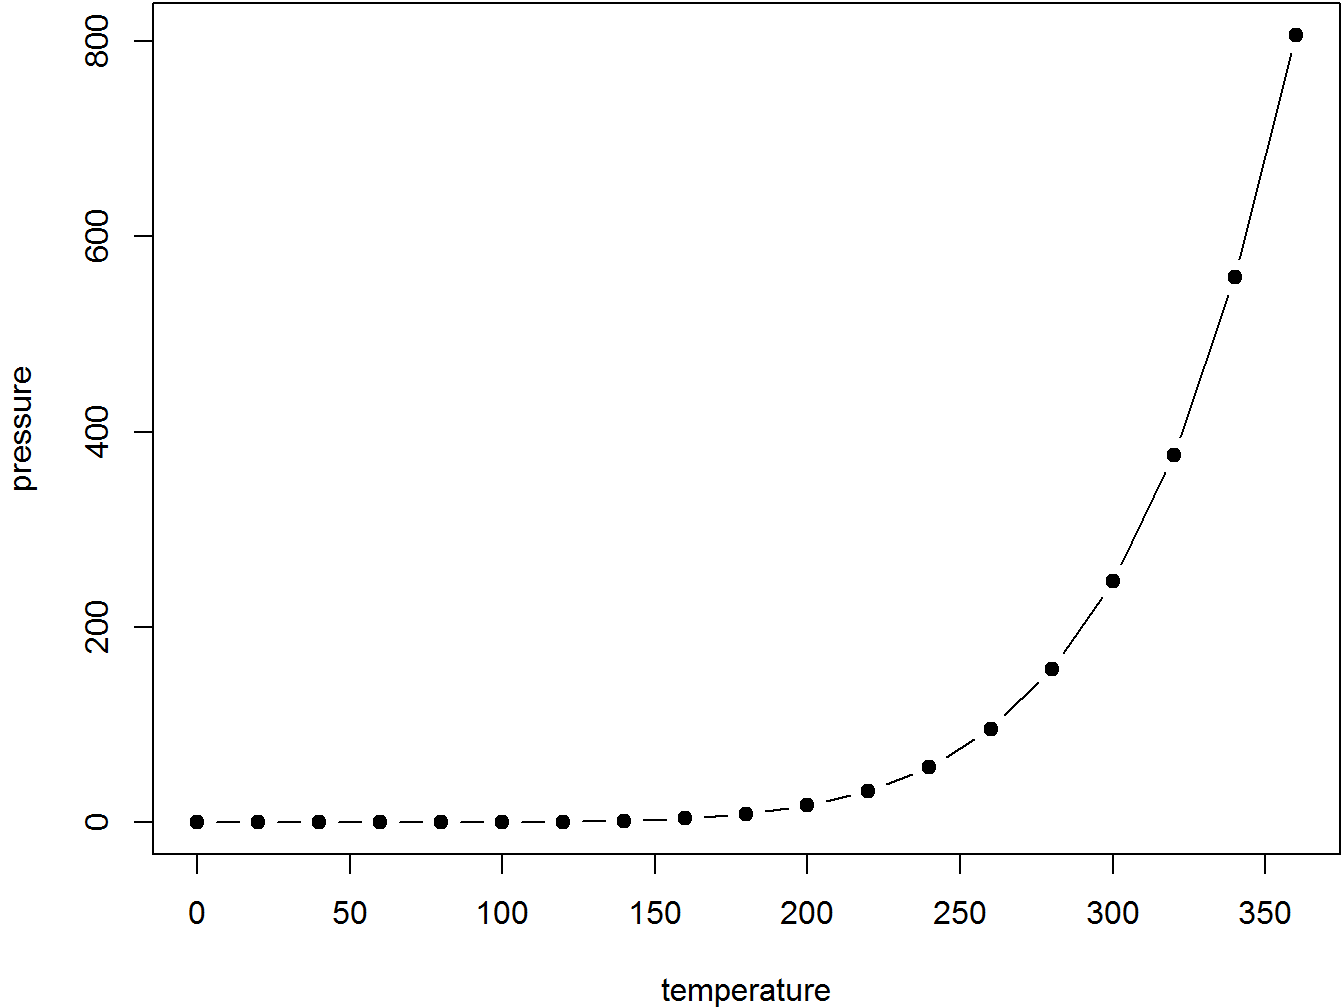
\includegraphics[width=0.9\linewidth]{bookdown_files/figure-latex/nice-fig-1} 

}

\caption{Here is a nice figure!}\label{fig:nice-fig}
\end{figure}

Reference a figure by its code chunk label with the \texttt{fig:}
prefix, e.g., see Figure \ref{fig:nice-fig}. Similarly, you can
reference tables generated from \texttt{knitr::kable()}, e.g., see Table
\ref{tab:nice-tab}.

\begin{Shaded}
\begin{Highlighting}[]
\NormalTok{knitr}\OperatorTok{::}\KeywordTok{kable}\NormalTok{(}
  \KeywordTok{head}\NormalTok{(iris, }\DecValTok{20}\NormalTok{), }\DataTypeTok{caption =} \StringTok{'Here is a nice table!'}\NormalTok{,}
  \DataTypeTok{booktabs =} \OtherTok{TRUE}
\NormalTok{)}
\end{Highlighting}
\end{Shaded}

\begin{table}

\caption{\label{tab:unnamed-chunk-5}Here is a nice table!}
\centering
\begin{tabular}[t]{rrrrl}
\toprule
Sepal.Length & Sepal.Width & Petal.Length & Petal.Width & Species\\
\midrule
5.1 & 3.5 & 1.4 & 0.2 & setosa\\
4.9 & 3.0 & 1.4 & 0.2 & setosa\\
4.7 & 3.2 & 1.3 & 0.2 & setosa\\
4.6 & 3.1 & 1.5 & 0.2 & setosa\\
5.0 & 3.6 & 1.4 & 0.2 & setosa\\
\addlinespace
5.4 & 3.9 & 1.7 & 0.4 & setosa\\
4.6 & 3.4 & 1.4 & 0.3 & setosa\\
5.0 & 3.4 & 1.5 & 0.2 & setosa\\
4.4 & 2.9 & 1.4 & 0.2 & setosa\\
4.9 & 3.1 & 1.5 & 0.1 & setosa\\
\addlinespace
5.4 & 3.7 & 1.5 & 0.2 & setosa\\
4.8 & 3.4 & 1.6 & 0.2 & setosa\\
4.8 & 3.0 & 1.4 & 0.1 & setosa\\
4.3 & 3.0 & 1.1 & 0.1 & setosa\\
5.8 & 4.0 & 1.2 & 0.2 & setosa\\
\addlinespace
5.7 & 4.4 & 1.5 & 0.4 & setosa\\
5.4 & 3.9 & 1.3 & 0.4 & setosa\\
5.1 & 3.5 & 1.4 & 0.3 & setosa\\
5.7 & 3.8 & 1.7 & 0.3 & setosa\\
5.1 & 3.8 & 1.5 & 0.3 & setosa\\
\bottomrule
\end{tabular}
\end{table}

You can write citations, too. For example, we are using the
\textbf{bookdown} package \citep{R-bookdown} in this sample book, which
was built on top of R Markdown and \textbf{knitr} \citep{xie2015}.

\mainmatter

\hypertarget{part-ng-dung-thc-t}{%
\part{Ứng dụng thực tế}\label{part-ng-dung-thc-t}}

\hypertarget{cac-phuong-phap-phan-tich-d-liu-thc-t-ng-dung-vi-r}{%
\chapter{Các phương pháp phân tích dữ liệu thực tế ứng dụng với
R}\label{cac-phuong-phap-phan-tich-d-liu-thc-t-ng-dung-vi-r}}

We talk about the \emph{FOO} method\index{FOO} in this chapter.

\hypertarget{phn-1}{%
\section{Phần 1}\label{phn-1}}

\hypertarget{phn-2}{%
\section{Phần 2}\label{phn-2}}

\hypertarget{phn-3}{%
\section{Phần 3}\label{phn-3}}

\hypertarget{ng-phap-cua-bin-i-d-liu-vi-dplyr}{%
\chapter{Ngữ pháp của biến đổi dữ liệu với
DPLYR}\label{ng-phap-cua-bin-i-d-liu-vi-dplyr}}

Khi bắt tay vào công việc phân tích số liệu, việc đầu tiên ta cần phải
làm là thu thập dữ liệu từ nhiều nguồn khác nhau. Sau khi hoàn thành
xong bước này, ta sẽ phải dành phần lớn thời gian để làm sạch, biến đổi
và tổng hợp dữ liệu nhằm tìm kiếm các insights hoặc chuẩn bị dữ liệu cho
các bước xây dựng mô hình, dự báo.

R rất mạnh trong việc biến đối dữ liệu và có rất nhiều package hỗ trợ
cho công việc này. Tuy nhiên, thư viện nổi tiếng nhất trong R trong việc
làm sạch và biến đổi dữ liệu là \texttt{dplyr}, một thư viện nổi tiếng
với những tính năng chuyên cho việc xử lý, tổng hợp dữ liệu trước khi
xây dựng mô hình phân tích dữ liệu. Chương này sẽ tập trung vào giới
thiệu về những hàm cơ bản nhất của \texttt{dplyr}.

Trước khi bắt đầu nội dung bài giảng, chúng ta có thể download và gọi
gói dplyr.

\begin{Shaded}
\begin{Highlighting}[]
\CommentTok{#install.packages("dplyr")}
\KeywordTok{library}\NormalTok{(dplyr)}
\end{Highlighting}
\end{Shaded}

\hypertarget{gii-thiu-v-pipe-operator}{%
\section{Giới thiệu về pipe operator}\label{gii-thiu-v-pipe-operator}}

Khi viết các câu lệnh, thông thường ta có 2 cách viết phổ biến sau.

\begin{itemize}
\item
  Cách 1: Viết với các câu lệnh lồng vào nhau (nested). Với cách viết
  này, các hàm sẽ được viết lồng vào nhau và kết quả của hàm sẽ được
  tính toán theo thứ tự từ trong ra ngoài.
\item
  Cách 2: Viết lưu dưới dạng các đối tượng trung gian. Với cách viết
  này, từng đối tượng sẽ được tính toán từng phần và kết quả sẽ được
  hiển thị một cách mạch lạc hơn. Tuy nhiên, nhược điểm của phương pháp
  này là sẽ tạo ra rất nhiều đối tượng trung gian, gây ra khó khăn trong
  việc theo dõi và quản lỹ.
\end{itemize}

Giả sử ta cần tính toán độ lệch chuẩn của véc-tơ x, công thức tính độ
lệch chuẩn sẽ là

\[\sigma = \frac{\sum_{i=1}^n(x_i-\overline{x})^2}{n-1}\]

Với hai cách viết code khác nhau, ta có thể tính độ lệch chuẩn theo hai
cách.

\begin{Shaded}
\begin{Highlighting}[]
\CommentTok{# Cách 1}
\CommentTok{# Tạo vector x}
\NormalTok{x <-}\StringTok{ }\KeywordTok{seq}\NormalTok{(}\DecValTok{2}\NormalTok{, }\DecValTok{100}\NormalTok{, }\DecValTok{2}\NormalTok{)  }
\CommentTok{# Tính độ lệch chuẩn}
\KeywordTok{sqrt}\NormalTok{(}\KeywordTok{sum}\NormalTok{((x}\OperatorTok{-}\KeywordTok{mean}\NormalTok{(x))}\OperatorTok{^}\DecValTok{2}\NormalTok{)}\OperatorTok{/}\NormalTok{(}\KeywordTok{length}\NormalTok{(x)}\OperatorTok{-}\DecValTok{1}\NormalTok{))}
\end{Highlighting}
\end{Shaded}

\begin{verbatim}
## [1] 29.15
\end{verbatim}

\begin{Shaded}
\begin{Highlighting}[]
\KeywordTok{sd}\NormalTok{(x)}
\end{Highlighting}
\end{Shaded}

\begin{verbatim}
## [1] 29.15
\end{verbatim}

\begin{Shaded}
\begin{Highlighting}[]
\CommentTok{# Cách 2}
\CommentTok{# Tạo vector x}
\NormalTok{x <-}\StringTok{ }\KeywordTok{seq}\NormalTok{(}\DecValTok{2}\NormalTok{, }\DecValTok{100}\NormalTok{, }\DecValTok{2}\NormalTok{)}
\CommentTok{# Tính tổng bình phương }
\NormalTok{sum_sqr <-}\StringTok{ }\KeywordTok{sum}\NormalTok{((x}\OperatorTok{-}\KeywordTok{mean}\NormalTok{(x))}\OperatorTok{^}\DecValTok{2}\NormalTok{)}
\NormalTok{len_x <-}\StringTok{ }\KeywordTok{length}\NormalTok{(x)}
\NormalTok{var <-}\StringTok{ }\NormalTok{sum_sqr}\OperatorTok{/}\NormalTok{(len_x }\OperatorTok{-}\StringTok{ }\DecValTok{1}\NormalTok{)}
\NormalTok{sd <-}\StringTok{ }\NormalTok{var}\OperatorTok{^}\NormalTok{(}\DecValTok{1}\OperatorTok{/}\DecValTok{2}\NormalTok{)}
\NormalTok{sd}
\end{Highlighting}
\end{Shaded}

\begin{verbatim}
## [1] 29.15
\end{verbatim}

Ta thấy kết quả ở hai cách tính là như nhau. Tuy nhiên, cách viết hai sẽ
tạo ra nhiều đối tượng trung gian hơn cách viết 1 rất nhiều. Khi phân
tích dữ liệu thực tế, ta sẽ phải áp dụng cả 2 cách viết code để có thể
vận dụng linh hoạt trong từng trường hợp cụ thể.

Trong R, có cách viết code thứ ba, được gọi là cách suwr dụng
\texttt{pipe\ operator} \texttt{(\%\textgreater{}\%)}.
\texttt{Toán\ tử\ Pipe} cho phép viết code theo cách đơn giản và dễ theo
dõi giúp cho người đọc và người viết code trên R có thể theo dõi được
code một cách dễ dàng nhất. Câu trúc của pipe như sau

\begin{quote}
f(x, y) = x \%\textgreater{}\% f(., y)
\end{quote}

Ví dụ của pipe.

\begin{Shaded}
\begin{Highlighting}[]
\CommentTok{# Cách 1}
\KeywordTok{mean}\NormalTok{(x)}
\CommentTok{# Cách 2}
\NormalTok{x }\OperatorTok\StringTok{ }\NormalTok{mean}
\end{Highlighting}
\end{Shaded}

Ta có thể xem xét ví dụ phức tạp hơn.

\begin{Shaded}
\begin{Highlighting}[]
\CommentTok{# Cách 1 - dùng cách viết thường}
\KeywordTok{summary}\NormalTok{(}\KeywordTok{head}\NormalTok{(iris))}
\end{Highlighting}
\end{Shaded}

\begin{verbatim}
##   Sepal.Length   Sepal.Width    Petal.Length 
##  Min.   :4.60   Min.   :3.00   Min.   :1.30  
##  1st Qu.:4.75   1st Qu.:3.12   1st Qu.:1.40  
##  Median :4.95   Median :3.35   Median :1.40  
##  Mean   :4.95   Mean   :3.38   Mean   :1.45  
##  3rd Qu.:5.08   3rd Qu.:3.58   3rd Qu.:1.48  
##  Max.   :5.40   Max.   :3.90   Max.   :1.70  
##   Petal.Width          Species 
##  Min.   :0.200   setosa    :6  
##  1st Qu.:0.200   versicolor:0  
##  Median :0.200   virginica :0  
##  Mean   :0.233                 
##  3rd Qu.:0.200                 
##  Max.   :0.400
\end{verbatim}

\begin{Shaded}
\begin{Highlighting}[]
\CommentTok{# Cách 2 - dùng pipe}
\NormalTok{iris }\OperatorTok\StringTok{ }\NormalTok{head }\OperatorTok\StringTok{ }\NormalTok{summary}
\end{Highlighting}
\end{Shaded}

\begin{verbatim}
##   Sepal.Length   Sepal.Width    Petal.Length 
##  Min.   :4.60   Min.   :3.00   Min.   :1.30  
##  1st Qu.:4.75   1st Qu.:3.12   1st Qu.:1.40  
##  Median :4.95   Median :3.35   Median :1.40  
##  Mean   :4.95   Mean   :3.38   Mean   :1.45  
##  3rd Qu.:5.08   3rd Qu.:3.58   3rd Qu.:1.48  
##  Max.   :5.40   Max.   :3.90   Max.   :1.70  
##   Petal.Width          Species 
##  Min.   :0.200   setosa    :6  
##  1st Qu.:0.200   versicolor:0  
##  Median :0.200   virginica :0  
##  Mean   :0.233                 
##  3rd Qu.:0.200                 
##  Max.   :0.400
\end{verbatim}

Cả hai cách đều cho ra kết quả giống nhau. Tuy nhiên, cách hai sẽ dễ
theo dõi, dễ đọc hơn cách 1 rất nhiều. Cách đọc hiểu quá trình thực hiện
pipe như sau:

\begin{enumerate}
\def\labelenumi{\arabic{enumi}.}
\tightlist
\item
  Gọi tập dữ liệu \texttt{iris} để phân tích
\item
  Thực hiện hàm \texttt{head} trên tập dữ liệu này, \emph{được kết quả
  bao nhiêu}\ldots{}
\item
  \ldots{} tiếp tục thực hiện hàm \texttt{summary}
\end{enumerate}

Như ta thấy, cách viết theo phong cách của
\texttt{pipe\ operator\ (\%\textgreater{}\%)} cho phép ta thực hiện các
phép tính theo đúng mạch tư duy logic của bản thân. Điều này là một điểm
rất mạnh mà hiện tại, mới chỉ ở R có toán tử \texttt{\%\textgreater{}\%}
áp dụng được cho mọi hàm.

\textbf{Một số đặc tính cơ bản của \texttt{\%\textgreater{}\%}}:

\begin{enumerate}
\def\labelenumi{\arabic{enumi}.}
\tightlist
\item
  Theo mặc định, Phía tay trái (LHS) sẽ được chuyển tiếp thành yếu tố
  đầu tiên của hàm được sử dụng phía tay phải (RHS), ví dụ:
\end{enumerate}

\begin{Shaded}
\begin{Highlighting}[]
\KeywordTok{mean}\NormalTok{(x) }
\end{Highlighting}
\end{Shaded}

\begin{verbatim}
## [1] 51
\end{verbatim}

\begin{Shaded}
\begin{Highlighting}[]
\CommentTok{# Tương đương với:}
\NormalTok{x }\OperatorTok\StringTok{ }\NormalTok{mean}
\end{Highlighting}
\end{Shaded}

\begin{verbatim}
## [1] 51
\end{verbatim}

\begin{enumerate}
\def\labelenumi{\arabic{enumi}.}
\setcounter{enumi}{1}
\tightlist
\item
  Khi LHS không còn là yếu tố đầu tiên của một hàm RHS, thì dấu ``.''
  được sử dụng để định vị cho LHS, ví dụ:
\end{enumerate}

\begin{Shaded}
\begin{Highlighting}[]
\KeywordTok{library}\NormalTok{(dplyr)}
\CommentTok{# Cách 1}
\KeywordTok{summary}\NormalTok{(}\KeywordTok{lm}\NormalTok{(mpg }\OperatorTok{~}\StringTok{ }\NormalTok{cyl, }\DataTypeTok{data =}\NormalTok{ mtcars))}

\CommentTok{# Cách 2}
\NormalTok{mtcars }\OperatorTok\StringTok{ }
\StringTok{  }\KeywordTok{lm}\NormalTok{(mpg }\OperatorTok{~}\StringTok{ }\NormalTok{cyl, }\DataTypeTok{data =}\NormalTok{ .) }\OperatorTok\StringTok{ }
\StringTok{  }\NormalTok{summary}
\end{Highlighting}
\end{Shaded}

Trong tình huống trên, tham số về dữ liệu trong hàm lm không phải là ở
đầu, mà sau phần công thức, nên chúng ta sẽ dùng dấu ``.'' như là đại
diện của thực thể mtcars ở bên ngoài (LHS) của hàm lm.

\hypertarget{cac-ham-co-ban-trong-dplyr}{%
\section{Các hàm cơ bản trong dplyr}\label{cac-ham-co-ban-trong-dplyr}}

Trong công việc biến đổi dữ liệu, bất kỳ ngôn ngữ phân tích nào cũng có
3 nhóm hàm lớn.

\begin{itemize}
\tightlist
\item
  Nhóm 1 - các hàm truy vấn dữ liệu: Lấy dữ liệu theo dòng, theo cột và
  theo điều kiện. Trong \texttt{dplyr} sẽ là các hàm \texttt{select},
  \texttt{filter} và \texttt{slice}
\item
  Nhóm 2 - Các hàm tổng hợp dữ liệu: Tính toán tổng hợp dữ liệu theo
  chiều. Trong \texttt{dplyr} sẽ là các hàm \texttt{group\_by},
  \texttt{summarise}
\item
  Nhóm 3 - Các hàm biến đổi dữ liệu: Tạo mới, biến đổi các dữ liệu cũ
  thành các dữ liệu mới. Trong \texttt{dplyr} sẽ là các hàm thuộc nhóm
  \texttt{mutate}, \texttt{join}, \texttt{bind}
\end{itemize}

Trong phần này, chúng ta sẽ giới thiệu nhanh các nhóm câu lệnh cơ bản
trên.

\hypertarget{nhom-cau-lnh-truy-vn-d-liu}{%
\subsection{Nhóm câu lệnh truy vấn dữ
liệu}\label{nhom-cau-lnh-truy-vn-d-liu}}

Khi truy vấn dữ liệu, ta thường phải thực hiện 3 nhóm công việc sau.

\begin{itemize}
\tightlist
\item
  Lấy theo cột
\item
  Lấy theo dòng
\item
  Lấy theo điều kiện
\end{itemize}

Xét về mặt bản chất, lấy theo điều kiện là một trường hợp đặc biệt của
việc lấy theo dòng. Đối với các ngôn ngữ như SQL, sẽ không phân biệt hai
loại này. Tuy nhiên, vì R lưu thứ tự của từng quan sát trong dataframe,
nên việc phân biệt được hai loại truy vấn trên là cần thiết.

\hypertarget{ly-cac-ct-trong-dataframe-vi-select}{%
\subsubsection{\texorpdfstring{Lấy các cột trong dataframe với
\texttt{select}}{Lấy các cột trong dataframe với select}}\label{ly-cac-ct-trong-dataframe-vi-select}}

\begin{quote}
data \%\textgreater{}\% select(var1, var2, \ldots{})
\end{quote}

Trong đó, \texttt{var1}, \texttt{var2} là tên các cột cần truy vấn. Đặc
biệt, R rất linh hoạt trong việc lọc theo cột. Ta có thể truy vấn theo
tên, theo thứ tự hoặc thậm chí theo các khoảng thứ tự các biến. Xem ví
dụ sau.

\begin{Shaded}
\begin{Highlighting}[]
\KeywordTok{library}\NormalTok{(dplyr)}
\CommentTok{# Xêm tên các biến trong mtcars}
\NormalTok{mtcars }\OperatorTok\StringTok{ }\NormalTok{names}
\end{Highlighting}
\end{Shaded}

\begin{verbatim}
##  [1] "mpg"  "cyl"  "disp" "hp"   "drat" "wt"   "qsec"
##  [8] "vs"   "am"   "gear" "carb"
\end{verbatim}

\begin{Shaded}
\begin{Highlighting}[]
\CommentTok{# Chọn cột mpg và cyl}
\NormalTok{mtcars }\OperatorTok\StringTok{ }\KeywordTok{select}\NormalTok{(mpg, cyl) }\OperatorTok\StringTok{ }\NormalTok{head}
\end{Highlighting}
\end{Shaded}

\begin{verbatim}
##                    mpg cyl
## Mazda RX4         21.0   6
## Mazda RX4 Wag     21.0   6
## Datsun 710        22.8   4
## Hornet 4 Drive    21.4   6
## Hornet Sportabout 18.7   8
## Valiant           18.1   6
\end{verbatim}

\begin{Shaded}
\begin{Highlighting}[]
\CommentTok{# Chọn cột thứ nhất và thứ hai}
\NormalTok{mtcars }\OperatorTok\StringTok{ }\KeywordTok{select}\NormalTok{(}\DecValTok{1}\NormalTok{,}\DecValTok{2}\NormalTok{) }\OperatorTok\StringTok{ }\NormalTok{head}
\end{Highlighting}
\end{Shaded}

\begin{verbatim}
##                    mpg cyl
## Mazda RX4         21.0   6
## Mazda RX4 Wag     21.0   6
## Datsun 710        22.8   4
## Hornet 4 Drive    21.4   6
## Hornet Sportabout 18.7   8
## Valiant           18.1   6
\end{verbatim}

\begin{Shaded}
\begin{Highlighting}[]
\CommentTok{# Chọn cột thứ 3 đến cột thứ 6}
\NormalTok{mtcars }\OperatorTok\StringTok{ }\KeywordTok{select}\NormalTok{(}\DecValTok{3}\OperatorTok{:}\DecValTok{6}\NormalTok{) }\OperatorTok\StringTok{ }\NormalTok{head}
\end{Highlighting}
\end{Shaded}

\begin{verbatim}
##                   disp  hp drat    wt
## Mazda RX4          160 110 3.90 2.620
## Mazda RX4 Wag      160 110 3.90 2.875
## Datsun 710         108  93 3.85 2.320
## Hornet 4 Drive     258 110 3.08 3.215
## Hornet Sportabout  360 175 3.15 3.440
## Valiant            225 105 2.76 3.460
\end{verbatim}

~

Ngoài ra, khi lấy chi tiết các cột (liệt kê từng cột) khi lấy dữ liệu
trên 1 bảng, bạn có thể dùng một số hàm sau để hỗ trợ việc lấy trường dữ
liệu được nhanh hơn:

\begin{itemize}
\tightlist
\item
  \texttt{starts\_with("Ký\ tự\ là\ thông\ tin\ mong\ muốn")}: các cột
  dữ liệu ccó tên hứa các ký tự mong muốn đứng ở đầu của tên, ví dụ:
\end{itemize}

\begin{Shaded}
\begin{Highlighting}[]
\NormalTok{iris }\OperatorTok
\StringTok{  }\KeywordTok{select}\NormalTok{(}\KeywordTok{starts_with}\NormalTok{(}\StringTok{"Petal"}\NormalTok{)) }\OperatorTok
\StringTok{  }\NormalTok{head}
\end{Highlighting}
\end{Shaded}

\begin{verbatim}
##   Petal.Length Petal.Width
## 1          1.4         0.2
## 2          1.4         0.2
## 3          1.3         0.2
## 4          1.5         0.2
## 5          1.4         0.2
## 6          1.7         0.4
\end{verbatim}

\begin{itemize}
\tightlist
\item
  \texttt{ends\_with("Ký\ tự\ là\ thông\ tin\ mong\ muốn")}: các cột dữ
  liệu có tên chứa các ký tự mong muốn ở cuối của tên, ví dụ:
\end{itemize}

\begin{Shaded}
\begin{Highlighting}[]
\NormalTok{iris }\OperatorTok
\StringTok{  }\KeywordTok{select}\NormalTok{(}\KeywordTok{ends_with}\NormalTok{(}\StringTok{"Length"}\NormalTok{)) }\OperatorTok
\StringTok{  }\NormalTok{head}
\end{Highlighting}
\end{Shaded}

\begin{verbatim}
##   Sepal.Length Petal.Length
## 1          5.1          1.4
## 2          4.9          1.4
## 3          4.7          1.3
## 4          4.6          1.5
## 5          5.0          1.4
## 6          5.4          1.7
\end{verbatim}

\begin{itemize}
\tightlist
\item
  \texttt{contains("Ký\ tự\ là\ thông\ tin\ mong\ muốn")}: các cột dữ
  liệu có tên chứa chính xác các ký tự mong muốn ở bất kỳ vị trí nào của
  tên, ví dụ:
\end{itemize}

\begin{Shaded}
\begin{Highlighting}[]
\NormalTok{iris }\OperatorTok
\StringTok{  }\KeywordTok{select}\NormalTok{(}\KeywordTok{contains}\NormalTok{(}\StringTok{"etal"}\NormalTok{)) }\OperatorTok
\StringTok{  }\NormalTok{head}
\end{Highlighting}
\end{Shaded}

\begin{verbatim}
##   Petal.Length Petal.Width
## 1          1.4         0.2
## 2          1.4         0.2
## 3          1.3         0.2
## 4          1.5         0.2
## 5          1.4         0.2
## 6          1.7         0.4
\end{verbatim}

\begin{itemize}
\tightlist
\item
  matches(``Dạng ký tự là thông tin mong muốn''): các cột dữ liệu có tên
  chứa các ký tự có dạng ký tự mong muốn ở bất kỳ vị trí nào của tên, ví
  dụ:
\end{itemize}

\begin{Shaded}
\begin{Highlighting}[]
\NormalTok{iris }\OperatorTok
\StringTok{  }\KeywordTok{select}\NormalTok{(}\KeywordTok{matches}\NormalTok{(}\StringTok{".t."}\NormalTok{)) }\OperatorTok\StringTok{ }
\StringTok{  }\NormalTok{head}
\end{Highlighting}
\end{Shaded}

\begin{verbatim}
##   Sepal.Length Sepal.Width Petal.Length Petal.Width
## 1          5.1         3.5          1.4         0.2
## 2          4.9         3.0          1.4         0.2
## 3          4.7         3.2          1.3         0.2
## 4          4.6         3.1          1.5         0.2
## 5          5.0         3.6          1.4         0.2
## 6          5.4         3.9          1.7         0.4
\end{verbatim}

Trong ví dụ trên, R sẽ lấy tất cả các cột có tên chứa chữ t và có ký tự
khác ở trước và sau (các ký tự chỉ chứa chữ t mà chữ t ở đâu hoặc cuối
tên sẽ không được tính vào)

Thêm vào đó, ta có thể đổi tên biến ngay trong khi lựa chọn các biến với
\texttt{select} như sau:

\begin{Shaded}
\begin{Highlighting}[]
\NormalTok{mtcars }\OperatorTok
\StringTok{  }\KeywordTok{select}\NormalTok{(}\StringTok{`}\DataTypeTok{miles per gallon}\StringTok{`}\NormalTok{ =}\StringTok{ }\NormalTok{mpg}
\NormalTok{         , }\DataTypeTok{cylinder =}\NormalTok{ cyl}
\NormalTok{         , }\DataTypeTok{weight =}\NormalTok{ wt) }\OperatorTok
\StringTok{  }\NormalTok{head}
\end{Highlighting}
\end{Shaded}

\begin{verbatim}
##                   miles per gallon cylinder weight
## Mazda RX4                     21.0        6  2.620
## Mazda RX4 Wag                 21.0        6  2.875
## Datsun 710                    22.8        4  2.320
## Hornet 4 Drive                21.4        6  3.215
## Hornet Sportabout             18.7        8  3.440
## Valiant                       18.1        6  3.460
\end{verbatim}

\hypertarget{ly-cac-dong-trong-dataframe-vi-slice}{%
\subsubsection{\texorpdfstring{Lấy các dòng trong dataframe với
\texttt{slice}}{Lấy các dòng trong dataframe với slice}}\label{ly-cac-dong-trong-dataframe-vi-slice}}

\begin{quote}
data \%\textgreater{}\% slice(observation)
\end{quote}

Tương tự như lấy theo cột, ta có thể lấy các dòng trong một dataframe.
Tuy nhiên, lưu ý hàm \texttt{slice} chỉ cho phép điều kiện lấy quan sát
là một véc-tơ. Xem ví dụ sau.

\begin{Shaded}
\begin{Highlighting}[]
\CommentTok{# Lấy dòng đầu tiên}
\NormalTok{mtcars }\OperatorTok\StringTok{ }\KeywordTok{slice}\NormalTok{(}\DecValTok{1}\NormalTok{)}
\end{Highlighting}
\end{Shaded}

\begin{verbatim}
## # A tibble: 1 x 11
##     mpg   cyl  disp    hp  drat    wt  qsec    vs
##   <dbl> <dbl> <dbl> <dbl> <dbl> <dbl> <dbl> <dbl>
## 1   21.    6.  160.  110.  3.90  2.62  16.5    0.
## # ... with 3 more variables: am <dbl>, gear <dbl>,
## #   carb <dbl>
\end{verbatim}

\begin{Shaded}
\begin{Highlighting}[]
\CommentTok{# Lấy dòng từ 1:3}
\NormalTok{mtcars }\OperatorTok\StringTok{ }\KeywordTok{slice}\NormalTok{(}\DecValTok{1}\OperatorTok{:}\DecValTok{3}\NormalTok{)}
\end{Highlighting}
\end{Shaded}

\begin{verbatim}
## # A tibble: 3 x 11
##     mpg   cyl  disp    hp  drat    wt  qsec    vs
##   <dbl> <dbl> <dbl> <dbl> <dbl> <dbl> <dbl> <dbl>
## 1  21.0    6.  160.  110.  3.90  2.62  16.5    0.
## 2  21.0    6.  160.  110.  3.90  2.88  17.0    0.
## 3  22.8    4.  108.   93.  3.85  2.32  18.6    1.
## # ... with 3 more variables: am <dbl>, gear <dbl>,
## #   carb <dbl>
\end{verbatim}

\begin{Shaded}
\begin{Highlighting}[]
\CommentTok{# Lấy dòng 1:3 và 5}
\NormalTok{mtcars }\OperatorTok\StringTok{ }\KeywordTok{slice}\NormalTok{(}\KeywordTok{c}\NormalTok{(}\DecValTok{1}\OperatorTok{:}\DecValTok{3}\NormalTok{,}\DecValTok{5}\NormalTok{))}
\end{Highlighting}
\end{Shaded}

\begin{verbatim}
## # A tibble: 4 x 11
##     mpg   cyl  disp    hp  drat    wt  qsec    vs
##   <dbl> <dbl> <dbl> <dbl> <dbl> <dbl> <dbl> <dbl>
## 1  21.0    6.  160.  110.  3.90  2.62  16.5    0.
## 2  21.0    6.  160.  110.  3.90  2.88  17.0    0.
## 3  22.8    4.  108.   93.  3.85  2.32  18.6    1.
## 4  18.7    8.  360.  175.  3.15  3.44  17.0    0.
## # ... with 3 more variables: am <dbl>, gear <dbl>,
## #   carb <dbl>
\end{verbatim}

\hypertarget{loc-quan-sat-theo-iu-kin-vi-filter}{%
\subsubsection{\texorpdfstring{Lọc quan sát theo điều kiện với
\texttt{filter}}{Lọc quan sát theo điều kiện với filter}}\label{loc-quan-sat-theo-iu-kin-vi-filter}}

\begin{quote}
data \%\textgreater{}\% filter(condition)
\end{quote}

Hàm filter cho phép ta sử dụng các điều kiện phức tạp để truy xuất dữ
liệu từ dataframe. Các điều kiện thường dùng bao gồm.

\begin{longtable}[]{@{}lll@{}}
\toprule
Dấu & Ký hiệu & Ví dụ\tabularnewline
\midrule
\endhead
Bằng & \texttt{==} & \texttt{7==8}\tabularnewline
Khác & \texttt{!=} & \texttt{7!=8}\tabularnewline
Lớn hơn & \texttt{\textgreater{}} &
\texttt{a\ \textgreater{}\ b}\tabularnewline
Lớn hơn hoặc bằng & \texttt{\textgreater{}=} &
\texttt{a\ \textgreater{}=\ b}\tabularnewline
Nhỏ hơn & \texttt{\textless{}} &
\texttt{a\ \textless{}\ b}\tabularnewline
Nhỏ hơn hoặc bằng & \texttt{\textless{}=} &
\texttt{a\ \textless{}=\ b}\tabularnewline
Và & \texttt{\&} &
\texttt{a\ \textgreater{}\ 7\ \&\ b\ \textless{}\ 9}\tabularnewline
\bottomrule
\end{longtable}

Xem ví dụ sau.

\begin{Shaded}
\begin{Highlighting}[]
\CommentTok{# Lọc điều kiện mpg > 20}
\NormalTok{mtcars }\OperatorTok
\StringTok{  }\KeywordTok{filter}\NormalTok{(mpg }\OperatorTok{>}\StringTok{ }\DecValTok{20}\NormalTok{) }\OperatorTok\StringTok{ }
\StringTok{  }\NormalTok{dim}
\end{Highlighting}
\end{Shaded}

\begin{verbatim}
## [1] 14 11
\end{verbatim}

\begin{Shaded}
\begin{Highlighting}[]
\CommentTok{# Lọc điều kiện mpg >20 hoặc mpg <18}
\NormalTok{mtcars }\OperatorTok\StringTok{ }
\StringTok{  }\KeywordTok{filter}\NormalTok{(mpg }\OperatorTok{>}\StringTok{ }\DecValTok{20} \OperatorTok{|}\StringTok{ }\NormalTok{mpg }\OperatorTok{<}\StringTok{ }\DecValTok{18}\NormalTok{) }\OperatorTok\StringTok{ }
\StringTok{  }\NormalTok{dim}
\end{Highlighting}
\end{Shaded}

\begin{verbatim}
## [1] 27 11
\end{verbatim}

\begin{Shaded}
\begin{Highlighting}[]
\CommentTok{# Lọc điều kiện mpg >=20 và cyl = 6}
\NormalTok{mtcars }\OperatorTok\StringTok{ }
\StringTok{  }\KeywordTok{filter}\NormalTok{(mpg }\OperatorTok{>}\StringTok{ }\DecValTok{20} \OperatorTok{&}\StringTok{ }\NormalTok{cyl }\OperatorTok{==}\StringTok{ }\DecValTok{6}\NormalTok{)}
\end{Highlighting}
\end{Shaded}

\begin{verbatim}
##    mpg cyl disp  hp drat    wt  qsec vs am gear carb
## 1 21.0   6  160 110 3.90 2.620 16.46  0  1    4    4
## 2 21.0   6  160 110 3.90 2.875 17.02  0  1    4    4
## 3 21.4   6  258 110 3.08 3.215 19.44  1  0    3    1
\end{verbatim}

\textbf{Lưu ý}: Khi điều kiện \emph{hoặc} là chuỗi các giá trị rời rạc
áp dụng cho cùng một trường, chúng ta có thể làm ngắn gọn hơn với cấu
trúc ``\%in\%'' thay vì cấu phải liệt kê tất cả các điều kiện đơn lẻ và
ngăn cách nhau bởi dấu ``\textbar{}'':

\begin{Shaded}
\begin{Highlighting}[]
\NormalTok{mtcars }\OperatorTok
\StringTok{ }\KeywordTok{filter}\NormalTok{(carb }\OperatorTok{==}\StringTok{ }\DecValTok{4} \OperatorTok{|}\StringTok{ }\NormalTok{carb }\OperatorTok{==}\StringTok{ }\DecValTok{3} \OperatorTok{|}\StringTok{ }\NormalTok{carb }\OperatorTok{==}\StringTok{ }\DecValTok{1}\NormalTok{)}
\end{Highlighting}
\end{Shaded}

\begin{verbatim}
##     mpg cyl  disp  hp drat    wt  qsec vs am gear carb
## 1  21.0   6 160.0 110 3.90 2.620 16.46  0  1    4    4
## 2  21.0   6 160.0 110 3.90 2.875 17.02  0  1    4    4
## 3  22.8   4 108.0  93 3.85 2.320 18.61  1  1    4    1
## 4  21.4   6 258.0 110 3.08 3.215 19.44  1  0    3    1
## 5  18.1   6 225.0 105 2.76 3.460 20.22  1  0    3    1
## 6  14.3   8 360.0 245 3.21 3.570 15.84  0  0    3    4
## 7  19.2   6 167.6 123 3.92 3.440 18.30  1  0    4    4
## 8  17.8   6 167.6 123 3.92 3.440 18.90  1  0    4    4
## 9  16.4   8 275.8 180 3.07 4.070 17.40  0  0    3    3
## 10 17.3   8 275.8 180 3.07 3.730 17.60  0  0    3    3
## 11 15.2   8 275.8 180 3.07 3.780 18.00  0  0    3    3
## 12 10.4   8 472.0 205 2.93 5.250 17.98  0  0    3    4
## 13 10.4   8 460.0 215 3.00 5.424 17.82  0  0    3    4
## 14 14.7   8 440.0 230 3.23 5.345 17.42  0  0    3    4
## 15 32.4   4  78.7  66 4.08 2.200 19.47  1  1    4    1
## 16 33.9   4  71.1  65 4.22 1.835 19.90  1  1    4    1
## 17 21.5   4 120.1  97 3.70 2.465 20.01  1  0    3    1
## 18 13.3   8 350.0 245 3.73 3.840 15.41  0  0    3    4
## 19 27.3   4  79.0  66 4.08 1.935 18.90  1  1    4    1
## 20 15.8   8 351.0 264 4.22 3.170 14.50  0  1    5    4
\end{verbatim}

Câu lệnh trên tương đương với:

\begin{Shaded}
\begin{Highlighting}[]
\NormalTok{mtcars }\OperatorTok
\StringTok{  }\KeywordTok{filter}\NormalTok{(carb }\OperatorTok\StringTok{ }\KeywordTok{c}\NormalTok{(}\DecValTok{1}\NormalTok{, }\DecValTok{3}\NormalTok{, }\DecValTok{4}\NormalTok{))}
\end{Highlighting}
\end{Shaded}

\hypertarget{sp-xp-d-liu-vi-arrange}{%
\subsubsection{\texorpdfstring{Sắp xếp dữ liệu với
\texttt{arrange}}{Sắp xếp dữ liệu với arrange}}\label{sp-xp-d-liu-vi-arrange}}

\begin{quote}
data \%\textgreater{}\% arrange(var1, var2)
\end{quote}

Ngoài việc lọc dữ liệu có điều kiện, chúng ta cũng thường xuyên thực
hiện việc sắp xếp dữ liệu theo một trật tự nhất định nào đó khi xem dữ
liệu. Hàm arrange() hỗ trợ công việc này. Cách thức sắp xếp dữ liệu mặc
định là từ nhỏ đến lớn.

\begin{Shaded}
\begin{Highlighting}[]
\NormalTok{mtcars }\OperatorTok
\StringTok{  }\KeywordTok{arrange}\NormalTok{(mpg) }\OperatorTok\StringTok{ }
\StringTok{  }\NormalTok{head}
\end{Highlighting}
\end{Shaded}

\begin{verbatim}
##    mpg cyl disp  hp drat    wt  qsec vs am gear carb
## 1 10.4   8  472 205 2.93 5.250 17.98  0  0    3    4
## 2 10.4   8  460 215 3.00 5.424 17.82  0  0    3    4
## 3 13.3   8  350 245 3.73 3.840 15.41  0  0    3    4
## 4 14.3   8  360 245 3.21 3.570 15.84  0  0    3    4
## 5 14.7   8  440 230 3.23 5.345 17.42  0  0    3    4
## 6 15.0   8  301 335 3.54 3.570 14.60  0  1    5    8
\end{verbatim}

Khi có nhiều biến cần được sắp xếp, hàm \texttt{arrange} sẽ ưu tiên các
biến theo thứ tự từ trái sang phải.

\begin{Shaded}
\begin{Highlighting}[]
\NormalTok{mtcars }\OperatorTok\StringTok{ }\KeywordTok{arrange}\NormalTok{(mpg, cyl)}
\end{Highlighting}
\end{Shaded}

\begin{verbatim}
##     mpg cyl  disp  hp drat    wt  qsec vs am gear carb
## 1  10.4   8 472.0 205 2.93 5.250 17.98  0  0    3    4
## 2  10.4   8 460.0 215 3.00 5.424 17.82  0  0    3    4
## 3  13.3   8 350.0 245 3.73 3.840 15.41  0  0    3    4
## 4  14.3   8 360.0 245 3.21 3.570 15.84  0  0    3    4
## 5  14.7   8 440.0 230 3.23 5.345 17.42  0  0    3    4
## 6  15.0   8 301.0 335 3.54 3.570 14.60  0  1    5    8
## 7  15.2   8 275.8 180 3.07 3.780 18.00  0  0    3    3
## 8  15.2   8 304.0 150 3.15 3.435 17.30  0  0    3    2
## 9  15.5   8 318.0 150 2.76 3.520 16.87  0  0    3    2
## 10 15.8   8 351.0 264 4.22 3.170 14.50  0  1    5    4
## 11 16.4   8 275.8 180 3.07 4.070 17.40  0  0    3    3
## 12 17.3   8 275.8 180 3.07 3.730 17.60  0  0    3    3
## 13 17.8   6 167.6 123 3.92 3.440 18.90  1  0    4    4
## 14 18.1   6 225.0 105 2.76 3.460 20.22  1  0    3    1
## 15 18.7   8 360.0 175 3.15 3.440 17.02  0  0    3    2
## 16 19.2   6 167.6 123 3.92 3.440 18.30  1  0    4    4
## 17 19.2   8 400.0 175 3.08 3.845 17.05  0  0    3    2
## 18 19.7   6 145.0 175 3.62 2.770 15.50  0  1    5    6
## 19 21.0   6 160.0 110 3.90 2.620 16.46  0  1    4    4
## 20 21.0   6 160.0 110 3.90 2.875 17.02  0  1    4    4
## 21 21.4   4 121.0 109 4.11 2.780 18.60  1  1    4    2
## 22 21.4   6 258.0 110 3.08 3.215 19.44  1  0    3    1
## 23 21.5   4 120.1  97 3.70 2.465 20.01  1  0    3    1
## 24 22.8   4 108.0  93 3.85 2.320 18.61  1  1    4    1
## 25 22.8   4 140.8  95 3.92 3.150 22.90  1  0    4    2
## 26 24.4   4 146.7  62 3.69 3.190 20.00  1  0    4    2
## 27 26.0   4 120.3  91 4.43 2.140 16.70  0  1    5    2
## 28 27.3   4  79.0  66 4.08 1.935 18.90  1  1    4    1
## 29 30.4   4  75.7  52 4.93 1.615 18.52  1  1    4    2
## 30 30.4   4  95.1 113 3.77 1.513 16.90  1  1    5    2
## 31 32.4   4  78.7  66 4.08 2.200 19.47  1  1    4    1
## 32 33.9   4  71.1  65 4.22 1.835 19.90  1  1    4    1
\end{verbatim}

\hypertarget{i-ten-bin-vi-rename}{%
\subsubsection{\texorpdfstring{Đổi tên biến với
\texttt{rename}}{Đổi tên biến với rename}}\label{i-ten-bin-vi-rename}}

\begin{quote}
data \%\textgreater{}\% rename(new\_var = old\_var)
\end{quote}

\begin{Shaded}
\begin{Highlighting}[]
\NormalTok{mtcars }\OperatorTok
\StringTok{  }\KeywordTok{rename}\NormalTok{(}\DataTypeTok{displacement =}\NormalTok{ disp,}
         \DataTypeTok{miles_per_gallon =}\NormalTok{ mpg) }\OperatorTok\StringTok{ }
\StringTok{  }\NormalTok{names}
\end{Highlighting}
\end{Shaded}

\begin{verbatim}
##  [1] "miles_per_gallon" "cyl"             
##  [3] "displacement"     "hp"              
##  [5] "drat"             "wt"              
##  [7] "qsec"             "vs"              
##  [9] "am"               "gear"            
## [11] "carb"
\end{verbatim}

\hypertarget{nhom-cau-lnh-bin-i-d-liu}{%
\subsection{Nhóm câu lệnh biến đổi dữ
liệu}\label{nhom-cau-lnh-bin-i-d-liu}}

\hypertarget{tao-mi-trung-d-liu-vi-mutate}{%
\paragraph{\texorpdfstring{Tạo mới trường dữ liệu với
\texttt{mutate}}{Tạo mới trường dữ liệu với mutate}}\label{tao-mi-trung-d-liu-vi-mutate}}

Trong quá trình xử lý dữ liệu, ta thường xuyên phải tạo thêm các trường
dữ liệu mới (trường dữ liệu phát sinh). Hàm mutate() được sử dụng để làm
công việc này. Cấu trúc của hàm rất đơn giản như sau.

\begin{quote}
data \%\textgreater{}\% mutate(new\_var = statement)
\end{quote}

Xem ví dụ sau

\begin{Shaded}
\begin{Highlighting}[]
\NormalTok{mtcars }\OperatorTok
\StringTok{  }\KeywordTok{select}\NormalTok{(mpg) }\OperatorTok
\StringTok{  }\KeywordTok{mutate}\NormalTok{(}\DataTypeTok{new_mpg =}\NormalTok{ mpg }\OperatorTok{*}\StringTok{ }\DecValTok{2}\NormalTok{) }\OperatorTok
\StringTok{  }\NormalTok{head}
\end{Highlighting}
\end{Shaded}

\begin{verbatim}
##    mpg new_mpg
## 1 21.0    42.0
## 2 21.0    42.0
## 3 22.8    45.6
## 4 21.4    42.8
## 5 18.7    37.4
## 6 18.1    36.2
\end{verbatim}

Trong một số trường hợp, khi ta không muốn lấy các trường thông tin cũ
mà chỉ muốn lấy các trường thông tin mới tạo thì có thể sử dụng hàm
\texttt{transmute()} với cấu trúc giống như hàm mutate.

\begin{Shaded}
\begin{Highlighting}[]
\NormalTok{mtcars }\OperatorTok
\StringTok{  }\KeywordTok{select}\NormalTok{(mpg) }\OperatorTok\StringTok{ }
\StringTok{  }\KeywordTok{transmute}\NormalTok{(}\DataTypeTok{new_mpg =}\NormalTok{ mpg }\OperatorTok{*}\StringTok{ }\FloatTok{1.61}\NormalTok{) }\OperatorTok
\StringTok{  }\NormalTok{head}
\end{Highlighting}
\end{Shaded}

\begin{verbatim}
##   new_mpg
## 1   33.81
## 2   33.81
## 3   36.71
## 4   34.45
## 5   30.11
## 6   29.14
\end{verbatim}

\hypertarget{gp-nhiu-bang-vi-nhom-ham-join}{%
\paragraph{\texorpdfstring{Gộp nhiều bảng với nhóm hàm
\texttt{join}}{Gộp nhiều bảng với nhóm hàm join}}\label{gp-nhiu-bang-vi-nhom-ham-join}}

\begin{itemize}
\tightlist
\item
  Hàm \texttt{inner\_join(x,\ y,\ by\ =\ "key")}: lấy tất cả dữ liệu có
  trên bảng hai bảng khi trùng key, ví dụ:
\end{itemize}

\begin{Shaded}
\begin{Highlighting}[]
\NormalTok{x <-}\StringTok{ }\KeywordTok{data.frame}\NormalTok{(}\DataTypeTok{student_id =} \KeywordTok{seq}\NormalTok{(}\DecValTok{1}\NormalTok{, }\DecValTok{10}\NormalTok{, }\DecValTok{1}\NormalTok{), }
                \DataTypeTok{maths =} \KeywordTok{c}\NormalTok{(}\DecValTok{10}\NormalTok{, }\DecValTok{8}\NormalTok{, }\DecValTok{7}\NormalTok{, }\DecValTok{6}\NormalTok{, }\FloatTok{7.8}\NormalTok{, }\DecValTok{4}\NormalTok{, }
                          \FloatTok{7.7}\NormalTok{, }\DecValTok{9}\NormalTok{, }\FloatTok{9.5}\NormalTok{, }\FloatTok{6.5}\NormalTok{))}
\NormalTok{y <-}\StringTok{ }\KeywordTok{data.frame}\NormalTok{(}\DataTypeTok{student_id =} \KeywordTok{seq}\NormalTok{(}\DecValTok{2}\NormalTok{, }\DecValTok{20}\NormalTok{, }\DecValTok{2}\NormalTok{), }
                \DataTypeTok{physics =} \KeywordTok{c}\NormalTok{(}\DecValTok{8}\NormalTok{, }\FloatTok{9.5}\NormalTok{, }\FloatTok{7.5}\NormalTok{, }\DecValTok{6}\NormalTok{, }\FloatTok{5.5}\NormalTok{, }
                            \FloatTok{6.5}\NormalTok{, }\FloatTok{7.8}\NormalTok{, }\FloatTok{8.2}\NormalTok{, }\DecValTok{8}\NormalTok{, }\FloatTok{7.5}\NormalTok{))}
\NormalTok{x}
\end{Highlighting}
\end{Shaded}

\begin{verbatim}
##    student_id maths
## 1           1  10.0
## 2           2   8.0
## 3           3   7.0
## 4           4   6.0
## 5           5   7.8
## 6           6   4.0
## 7           7   7.7
## 8           8   9.0
## 9           9   9.5
## 10         10   6.5
\end{verbatim}

\begin{Shaded}
\begin{Highlighting}[]
\NormalTok{y}
\end{Highlighting}
\end{Shaded}

\begin{verbatim}
##    student_id physics
## 1           2     8.0
## 2           4     9.5
## 3           6     7.5
## 4           8     6.0
## 5          10     5.5
## 6          12     6.5
## 7          14     7.8
## 8          16     8.2
## 9          18     8.0
## 10         20     7.5
\end{verbatim}

\begin{Shaded}
\begin{Highlighting}[]
\CommentTok{# gộp 2 bảng dữ liệu x và y theo student_id}
\NormalTok{x }\OperatorTok
\StringTok{  }\KeywordTok{inner_join}\NormalTok{(y, }\DataTypeTok{by =} \StringTok{"student_id"}\NormalTok{) }
\end{Highlighting}
\end{Shaded}

\begin{verbatim}
##   student_id maths physics
## 1          2   8.0     8.0
## 2          4   6.0     9.5
## 3          6   4.0     7.5
## 4          8   9.0     6.0
## 5         10   6.5     5.5
\end{verbatim}

\begin{center}\rule{0.5\linewidth}{\linethickness}\end{center}

\begin{itemize}
\tightlist
\item
  \textbf{full\_join}: lấy tất cả dữ liệu có cả trên bảng x, y.
\end{itemize}

\begin{quote}
full\_join(x, y, by = ``key'')
\end{quote}

\begin{Shaded}
\begin{Highlighting}[]
\NormalTok{x }\OperatorTok
\StringTok{  }\KeywordTok{full_join}\NormalTok{(y, }\DataTypeTok{by =} \StringTok{"student_id"}\NormalTok{)}
\end{Highlighting}
\end{Shaded}

\begin{verbatim}
##    student_id maths physics
## 1           1  10.0      NA
## 2           2   8.0     8.0
## 3           3   7.0      NA
## 4           4   6.0     9.5
## 5           5   7.8      NA
## 6           6   4.0     7.5
## 7           7   7.7      NA
## 8           8   9.0     6.0
## 9           9   9.5      NA
## 10         10   6.5     5.5
## 11         12    NA     6.5
## 12         14    NA     7.8
## 13         16    NA     8.2
## 14         18    NA     8.0
## 15         20    NA     7.5
\end{verbatim}

Trong ví dụ trên, các giá trị về điểm toán (maths) sẽ trả về NA cho các
student\_id không tồn tại trên bảng y và ngược lại cho bảng x với các
giá trị điểm vật lý (physics) của các student\_id không tồn tại trên
bảng x.

\begin{center}\rule{0.5\linewidth}{\linethickness}\end{center}

\begin{itemize}
\tightlist
\item
  Hàm \textbf{left\_join}: lấy dữ liệu chỉ có trên bảng x, ví dụ:
\end{itemize}

\begin{quote}
left\_join(x, y, by = ``var'')
\end{quote}

\begin{Shaded}
\begin{Highlighting}[]
\NormalTok{x }\OperatorTok
\StringTok{  }\KeywordTok{left_join}\NormalTok{(y, }\DataTypeTok{by =} \StringTok{"student_id"}\NormalTok{) }
\end{Highlighting}
\end{Shaded}

\begin{verbatim}
##    student_id maths physics
## 1           1  10.0      NA
## 2           2   8.0     8.0
## 3           3   7.0      NA
## 4           4   6.0     9.5
## 5           5   7.8      NA
## 6           6   4.0     7.5
## 7           7   7.7      NA
## 8           8   9.0     6.0
## 9           9   9.5      NA
## 10         10   6.5     5.5
\end{verbatim}

Với các \texttt{student\_id} không có giá trị trên bảng y, cột physics
sẽ trả về giá trị NA

\begin{center}\rule{0.5\linewidth}{\linethickness}\end{center}

\begin{itemize}
\tightlist
\item
  Hàm \textbf{right\_join} : lấy dữ liệu chỉ có trên bảng y, ví dụ:
\end{itemize}

\begin{quote}
right\_join(x, y, by = ``var'')
\end{quote}

\begin{Shaded}
\begin{Highlighting}[]
\NormalTok{x }\OperatorTok
\StringTok{  }\KeywordTok{right_join}\NormalTok{(y, }\DataTypeTok{by =} \StringTok{"student_id"}\NormalTok{) }
\end{Highlighting}
\end{Shaded}

\begin{verbatim}
##    student_id maths physics
## 1           2   8.0     8.0
## 2           4   6.0     9.5
## 3           6   4.0     7.5
## 4           8   9.0     6.0
## 5          10   6.5     5.5
## 6          12    NA     6.5
## 7          14    NA     7.8
## 8          16    NA     8.2
## 9          18    NA     8.0
## 10         20    NA     7.5
\end{verbatim}

Với các \texttt{student\_id} không có giá trị trên bảng x, cột maths sẽ
trả về giá trị NA

\textbf{Lưu ý}: Trong trường hợp cột dữ liệu dùng để nối các bảng có tên
khác nhau, ta có thể sử dụng cấu trúc sau:

\begin{quote}
left\_join(x, y, by = c(``key\_x'' = ``key\_y''))
\end{quote}

Xem ví dụ sau:

\begin{Shaded}
\begin{Highlighting}[]
\KeywordTok{names}\NormalTok{(x)[}\DecValTok{1}\NormalTok{] <-}\StringTok{ "student_id1"}
\KeywordTok{names}\NormalTok{(y)[}\DecValTok{1}\NormalTok{] <-}\StringTok{ "student_id2"}

\NormalTok{x }\OperatorTok
\StringTok{  }\KeywordTok{inner_join}\NormalTok{(y, }\DataTypeTok{by =} \KeywordTok{c}\NormalTok{(}\StringTok{"student_id1"}\NormalTok{ =}\StringTok{ "student_id2"}\NormalTok{)) }
\end{Highlighting}
\end{Shaded}

\begin{verbatim}
##   student_id1 maths physics
## 1           2   8.0     8.0
## 2           4   6.0     9.5
## 3           6   4.0     7.5
## 4           8   9.0     6.0
## 5          10   6.5     5.5
\end{verbatim}

\hypertarget{ghep-nhiu-bang-theo-dong-hoc-ct-vi-nhom-ham-bind}{%
\paragraph{\texorpdfstring{Ghép nhiều bảng theo dòng hoặc cột với nhóm
hàm
\texttt{bind}}{Ghép nhiều bảng theo dòng hoặc cột với nhóm hàm bind}}\label{ghep-nhiu-bang-theo-dong-hoc-ct-vi-nhom-ham-bind}}

Bên cạnh các hàm \texttt{join}, khi xử lý dữ liệu trong thực tiễn, ta có
thể phải \emph{ghép} các bảng dữ liệu theo hàng hoặc cột. Trong dplyr,
có hai hàm rất hữu dụng trong hai trường hợp trên là \texttt{bind\_col}
và \texttt{bind\_rows}

\begin{quote}
bind\_cols(data1, data2) bind\_rows(data1, data2)
\end{quote}

Xem hai ví dụ sau.

\begin{Shaded}
\begin{Highlighting}[]
\NormalTok{df1 <-}\StringTok{ }\KeywordTok{data.frame}\NormalTok{(}\DataTypeTok{id =} \DecValTok{1}\OperatorTok{:}\DecValTok{3}\NormalTok{,}
                  \DataTypeTok{income =} \DecValTok{8}\OperatorTok{:}\DecValTok{10}\NormalTok{)}
\NormalTok{df2 <-}\StringTok{ }\KeywordTok{data.frame}\NormalTok{(}\DataTypeTok{id =} \DecValTok{4}\OperatorTok{:}\DecValTok{9}\NormalTok{,}
                  \DataTypeTok{income =} \DecValTok{8}\OperatorTok{:}\DecValTok{13}\NormalTok{)}
\NormalTok{df3 <-}\StringTok{ }\KeywordTok{data.frame}\NormalTok{(}\DataTypeTok{id =} \DecValTok{1}\OperatorTok{:}\DecValTok{3}\NormalTok{,}
                  \DataTypeTok{gender =} \KeywordTok{c}\NormalTok{(}\StringTok{"F"}\NormalTok{, }\StringTok{"F"}\NormalTok{, }\StringTok{"M"}\NormalTok{))}

\CommentTok{# Nối theo dòng}
\NormalTok{df1 }\OperatorTok\StringTok{ }\KeywordTok{bind_rows}\NormalTok{(df2)}
\end{Highlighting}
\end{Shaded}

\begin{verbatim}
##   id income
## 1  1      8
## 2  2      9
## 3  3     10
## 4  4      8
## 5  5      9
## 6  6     10
## 7  7     11
## 8  8     12
## 9  9     13
\end{verbatim}

\begin{Shaded}
\begin{Highlighting}[]
\CommentTok{# Nối theo cột}
\NormalTok{df1 }\OperatorTok\StringTok{ }\KeywordTok{bind_cols}\NormalTok{(df3)}
\end{Highlighting}
\end{Shaded}

\begin{verbatim}
##   id income id1 gender
## 1  1      8   1      F
## 2  2      9   2      F
## 3  3     10   3      M
\end{verbatim}

\hypertarget{nhom-ham-tng-hp-d-liu-vi-summarise}{%
\subsection{\texorpdfstring{Nhóm hàm tổng hợp dữ liệu với
\texttt{summarise}}{Nhóm hàm tổng hợp dữ liệu với summarise}}\label{nhom-ham-tng-hp-d-liu-vi-summarise}}

Trong quá trình xử lý dữ liệu, ta thường xuyên phải tổng hợp dữ liệu
theo các cách như: tính tổng, tính số dư bình quân, phương sai, tổng số
lượng quan sát\ldots{} Với \texttt{dplyr}, ta có thể sử dụng hàm
\texttt{summarise()} để thực hiện công việc này.

\begin{quote}
data \%\textgreater{}\% summarise(var\_name = calculate\_stats(var))
\end{quote}

\begin{Shaded}
\begin{Highlighting}[]
\NormalTok{mtcars }\OperatorTok\StringTok{ }
\StringTok{  }\KeywordTok{summarise}\NormalTok{(}\DataTypeTok{mean_mpg =} \KeywordTok{mean}\NormalTok{(mpg),}
            \DataTypeTok{sd_mpg =} \KeywordTok{sd}\NormalTok{(mpg))}
\end{Highlighting}
\end{Shaded}

\begin{verbatim}
##   mean_mpg sd_mpg
## 1    20.09  6.027
\end{verbatim}

Đây là ví dụ đơn giản nhất với \texttt{summarise} mà ta có thể thay thế
bằng \texttt{summary()} trên R base. Tuy nhiên, kết hợp giữa hàm
\texttt{summarise()} và hàm group\_by() trên dplyr sẽ cho chúng ta có
cái nhìn về dữ liệu tổng hợp một cách đa chiều hơn. Hàm group\_by() cho
phép dữ liệu tổng hợp được gộp lại theo một hoặc nhiều trường thông tin
khác nhau, giúp người phân tích có thể nhìn dữ liệu theo từ chiều riêng
biệt hoặc gộp các chiều thông tin với nhau.

\begin{Shaded}
\begin{Highlighting}[]
\NormalTok{mtcars }\OperatorTok\StringTok{ }
\StringTok{  }\KeywordTok{group_by}\NormalTok{(cyl) }\OperatorTok\StringTok{ }
\StringTok{  }\KeywordTok{summarise}\NormalTok{(}\DataTypeTok{mean_mpg =} \KeywordTok{mean}\NormalTok{(mpg),}
            \DataTypeTok{mean_disp =} \KeywordTok{mean}\NormalTok{(disp))}
\end{Highlighting}
\end{Shaded}

\begin{verbatim}
## # A tibble: 3 x 3
##     cyl mean_mpg mean_disp
##   <dbl>    <dbl>     <dbl>
## 1    4.     26.7      105.
## 2    6.     19.7      183.
## 3    8.     15.1      353.
\end{verbatim}

\hypertarget{cac-ham-nang-cao-trong-dplyr}{%
\section{Các hàm nâng cao trong
dplyr}\label{cac-ham-nang-cao-trong-dplyr}}

Bên cạnh các nhóm hàm cơ bản đã trình bày ở phần trên, \texttt{dplyr}
còn có một số hàm nâng cao khác đặc biệt hữu dụng trong quá trình biến
đổi, tổng hợp dữ liệu, bao gồm \texttt{case\_when}, \texttt{mutate\_at}
\& \texttt{summarise\_at}

\hypertarget{iu-kin-phan-nhom-vi-case_when}{%
\subsection{\texorpdfstring{Điều kiện phân nhóm với
\texttt{case\_when}}{Điều kiện phân nhóm với case\_when}}\label{iu-kin-phan-nhom-vi-case_when}}

Trong quá trình phân tích và xử lý dữ liệu, chúng ta thường phải tạo
thêm các trường mới hoặc tính toán dữ liệu dựa vào từng điều kiện khác
nhau để đưa ra giá trị của trường hoặc cách tính cho dữ liệu. Ví dụ, khi
ta muốn tính thưởng cho KH thì sẽ phải dùng nhiều công thức khác nhau
như KH thuộc VIP sẽ nhân 1 tỷ lệ, KH thuộc nhóm trung bình sẽ có 1 tỷ lệ
khác, hay KH thông thường thì sẽ 1 tỷ lệ khác\ldots{}.

Trong dplyr, hàm \texttt{case\_when()} xử lý các trường hợp trên rất
nhanh chóng.

\begin{quote}
data \%\textgreater{}\% mutate(new\_var = case\_when( condition\_1
\textasciitilde{} ``value\_1'', condition\_2 \textasciitilde{}
``value\_2'',\ldots{}, TRUE \textasciitilde{} ``value\_n'' ))
\end{quote}

Ta xem ví dụ sau:

\begin{Shaded}
\begin{Highlighting}[]
\NormalTok{df <-}\StringTok{ }\KeywordTok{data.frame}\NormalTok{(}\DataTypeTok{number =} \DecValTok{1}\OperatorTok{:}\DecValTok{10}\NormalTok{) }

\NormalTok{df }\OperatorTok\StringTok{ }\KeywordTok{mutate}\NormalTok{(}\DataTypeTok{nhom =} \KeywordTok{case_when}\NormalTok{(}
\NormalTok{  number }\OperatorTok{<=}\StringTok{ }\DecValTok{5} \OperatorTok{~}\StringTok{ "nhom_1"}\NormalTok{, }\CommentTok{# nhóm 1: số từ 1 đến 5}
\NormalTok{  number }\OperatorTok{>}\StringTok{ }\DecValTok{5} \OperatorTok{&}\StringTok{ }\NormalTok{number }\OperatorTok{<=}\StringTok{ }\DecValTok{8} \OperatorTok{~}\StringTok{ "nhom_2"}\NormalTok{, }\CommentTok{# nhóm 2: số từ 6 đến 8}
  \OtherTok{TRUE} \OperatorTok{~}\StringTok{ "nhom_3"} \CommentTok{# các số còn lại}
\NormalTok{  ))}
\end{Highlighting}
\end{Shaded}

\begin{verbatim}
##    number   nhom
## 1       1 nhom_1
## 2       2 nhom_1
## 3       3 nhom_1
## 4       4 nhom_1
## 5       5 nhom_1
## 6       6 nhom_2
## 7       7 nhom_2
## 8       8 nhom_2
## 9       9 nhom_3
## 10     10 nhom_3
\end{verbatim}

\hypertarget{tao-them-bin-mi-theo-iu-kin-vi-mutate_if-mutate_at}{%
\subsection{\texorpdfstring{Tạo thêm biến mới theo điều kiện với
\texttt{mutate\_if} \&
\texttt{mutate\_at}}{Tạo thêm biến mới theo điều kiện với mutate\_if \& mutate\_at}}\label{tao-them-bin-mi-theo-iu-kin-vi-mutate_if-mutate_at}}

Khi phân tích, ta có thể tạo thêm biến mới khi các biến trong dataframe
thỏa mãn điều kiện nào đó.

\begin{quote}
data \%\textgreater{}\% mutate\_if(condition, function)
\end{quote}

\begin{Shaded}
\begin{Highlighting}[]
\NormalTok{df <-}\StringTok{ }\KeywordTok{data.frame}\NormalTok{(}
  \DataTypeTok{id =} \DecValTok{1}\OperatorTok{:}\DecValTok{5}\NormalTok{,}
  \DataTypeTok{gender =} \KeywordTok{c}\NormalTok{(}\StringTok{"F"}\NormalTok{, }\StringTok{"M"}\NormalTok{, }\StringTok{"M"}\NormalTok{, }\StringTok{"F"}\NormalTok{, }\StringTok{"F"}\NormalTok{),}
  \DataTypeTok{income =} \KeywordTok{c}\NormalTok{(}\DecValTok{4}\NormalTok{,}\DecValTok{5}\NormalTok{,}\DecValTok{3}\NormalTok{,}\DecValTok{6}\NormalTok{,}\DecValTok{7}\NormalTok{)}
\NormalTok{)}
\NormalTok{df }\OperatorTok\StringTok{ }\NormalTok{summary}
\end{Highlighting}
\end{Shaded}

\begin{verbatim}
##        id    gender     income 
##  Min.   :1   F:3    Min.   :3  
##  1st Qu.:2   M:2    1st Qu.:4  
##  Median :3          Median :5  
##  Mean   :3          Mean   :5  
##  3rd Qu.:4          3rd Qu.:6  
##  Max.   :5          Max.   :7
\end{verbatim}

\begin{Shaded}
\begin{Highlighting}[]
\CommentTok{# Biến đổi các biến factor thành character}
\NormalTok{df }\OperatorTok\StringTok{ }\KeywordTok{mutate_if}\NormalTok{(is.factor, }
\NormalTok{                 as.character) }\OperatorTok\StringTok{ }
\StringTok{  }\NormalTok{summary}
\end{Highlighting}
\end{Shaded}

\begin{verbatim}
##        id       gender              income 
##  Min.   :1   Length:5           Min.   :3  
##  1st Qu.:2   Class :character   1st Qu.:4  
##  Median :3   Mode  :character   Median :5  
##  Mean   :3                      Mean   :5  
##  3rd Qu.:4                      3rd Qu.:6  
##  Max.   :5                      Max.   :7
\end{verbatim}

Ngoài ra, ta có thể tự tạo các hàm mới và áp dụng với
\texttt{mutate\_if}. Xem ví dụ sau.

\begin{Shaded}
\begin{Highlighting}[]
\NormalTok{my_func <-}\StringTok{ }\ControlFlowTok{function}\NormalTok{(x)\{x}\OperatorTok{*}\DecValTok{100}\NormalTok{\}}
\CommentTok{# Nhân các biến numeric lên 100 lần}
\NormalTok{df }\OperatorTok\StringTok{ }
\StringTok{  }\KeywordTok{mutate_if}\NormalTok{(is.numeric, my_func)}
\end{Highlighting}
\end{Shaded}

\begin{verbatim}
##    id gender income
## 1 100      F    400
## 2 200      M    500
## 3 300      M    300
## 4 400      F    600
## 5 500      F    700
\end{verbatim}

Đối với \texttt{mutate\_at}, ta cũng có thể thực hiện tương tự. Cấu trúc
tổng quát của \texttt{mutate\_at} như sau.

\begin{quote}
data \%\textgreater{}\% mutate\_at(vars(var1, var2, \ldots{}), function)
\end{quote}

\begin{Shaded}
\begin{Highlighting}[]
\NormalTok{df }
\end{Highlighting}
\end{Shaded}

\begin{verbatim}
##   id gender income
## 1  1      F      4
## 2  2      M      5
## 3  3      M      3
## 4  4      F      6
## 5  5      F      7
\end{verbatim}

\begin{Shaded}
\begin{Highlighting}[]
\CommentTok{# Nhân biến income lên 100 lần}
\NormalTok{df }\OperatorTok\StringTok{ }\KeywordTok{mutate_at}\NormalTok{(}\KeywordTok{vars}\NormalTok{(income), my_func)}
\end{Highlighting}
\end{Shaded}

\begin{verbatim}
##   id gender income
## 1  1      F    400
## 2  2      M    500
## 3  3      M    300
## 4  4      F    600
## 5  5      F    700
\end{verbatim}

\hypertarget{tng-hp-d-liu-theo-iu-kin-vi-summarise_at-va-summarise_if}{%
\subsection{\texorpdfstring{Tổng hợp dữ liệu theo điều kiện với
\texttt{summarise\_at} và
\texttt{summarise\_if}}{Tổng hợp dữ liệu theo điều kiện với summarise\_at và summarise\_if}}\label{tng-hp-d-liu-theo-iu-kin-vi-summarise_at-va-summarise_if}}

Tương tự như \texttt{mutate\_at} và \texttt{mutate\_if}, ta có thể tổng
hợp nhanh dữ liệu theo điều kiện.

Cấu trúc tổng quát của \texttt{summarise\_at}

\begin{quote}
data \%\textgreater{}\% group\_by(var) (không bắt buộc)
summarise\_at(vars(variables), funs(functions))
\end{quote}

Xem ví dụ sau

\begin{Shaded}
\begin{Highlighting}[]
\NormalTok{mtcars }\OperatorTok\StringTok{ }
\StringTok{  }\KeywordTok{group_by}\NormalTok{(am) }\OperatorTok\StringTok{ }
\StringTok{  }\KeywordTok{summarise_at}\NormalTok{(}\KeywordTok{vars}\NormalTok{(mpg, disp),}
               \KeywordTok{funs}\NormalTok{(mean, max, median))}
\end{Highlighting}
\end{Shaded}

\begin{verbatim}
## # A tibble: 2 x 7
##      am mpg_mean disp_mean mpg_max disp_max mpg_median
##   <dbl>    <dbl>     <dbl>   <dbl>    <dbl>      <dbl>
## 1    0.     17.1      290.    24.4     472.       17.3
## 2    1.     24.4      144.    33.9     351.       22.8
## # ... with 1 more variable: disp_median <dbl>
\end{verbatim}

Tương tự, ta có cấu trúc tổng quát của \texttt{summarise\_if}

\begin{quote}
data \%\textgreater{}\% group\_by(var) (không bắt buộc)
summarise\_if(condition, funs(functions))
\end{quote}

\begin{Shaded}
\begin{Highlighting}[]
\NormalTok{iris }\OperatorTok\StringTok{ }
\StringTok{  }\KeywordTok{select}\NormalTok{(Species, Sepal.Length, Sepal.Width) }\OperatorTok\StringTok{ }
\StringTok{  }\KeywordTok{group_by}\NormalTok{(Species) }\OperatorTok\StringTok{ }
\StringTok{  }\KeywordTok{summarise_if}\NormalTok{(is.numeric,}
               \KeywordTok{funs}\NormalTok{(mean, median))}
\end{Highlighting}
\end{Shaded}

\begin{verbatim}
## # A tibble: 3 x 5
##   Species    Sepal.Length_mean Sepal.Width_mean
##   <fct>                  <dbl>            <dbl>
## 1 setosa                  5.01             3.43
## 2 versicolor              5.94             2.77
## 3 virginica               6.59             2.97
## # ... with 2 more variables:
## #   Sepal.Length_median <dbl>,
## #   Sepal.Width_median <dbl>
\end{verbatim}

\hypertarget{phan-ra-va-xoay-chiu-d-liu}{%
\chapter{Phân rã và xoay chiều dữ
liệu}\label{phan-ra-va-xoay-chiu-d-liu}}

Khi phân tích dữ liệu, dữ liệu sau khi được làm sạch thường cơ bản có
hai dạng.

\begin{itemize}
\tightlist
\item
  Dạng ngang: Mỗi dòng ứng với 1 quan sát và nhiều biến
\item
  Dạng dọc: Nhiều dòng có thể chứa cùng một quan sát nhưng với các biến
  khác nhau.
\end{itemize}

Xem hai ví dụ về dữ liệu dạng ngang và dọc ở dưới đây.

\begin{tabular}{rlrrrr}
\toprule
id & Species & Sepal.Length & Sepal.Width & Petal.Length & Petal.Width\\
\midrule
1 & setosa & 5.1 & 3.5 & 1.4 & 0.2\\
2 & setosa & 4.9 & 3.0 & 1.4 & 0.2\\
3 & setosa & 4.7 & 3.2 & 1.3 & 0.2\\
4 & setosa & 4.6 & 3.1 & 1.5 & 0.2\\
5 & setosa & 5.0 & 3.6 & 1.4 & 0.2\\
6 & setosa & 5.4 & 3.9 & 1.7 & 0.4\\
\bottomrule
\end{tabular}

\begin{tabular}{rllr}
\toprule
id & Species & Measurement & Value\\
\midrule
1 & setosa & Sepal.Length & 5.1\\
1 & setosa & Sepal.Width & 3.5\\
1 & setosa & Petal.Length & 1.4\\
1 & setosa & Petal.Width & 0.2\\
2 & setosa & Sepal.Length & 4.9\\
\addlinespace
2 & setosa & Sepal.Width & 3.0\\
2 & setosa & Petal.Length & 1.4\\
2 & setosa & Petal.Width & 0.2\\
\bottomrule
\end{tabular}

Trong thực tế, chúng ta phải sử dụng rất linh hoạt cả hai định dạng dữ
liệu này (dữ liệu ngang và dữ liệu dọc). Trong chương này, chúng ta sẽ
học cách sử dụng và biến đổi dữ liệu giữa hai định dạng với
\texttt{tidyr}.

\hypertarget{phan-ra-d-liu-thanh-dang-doc-vi-gather}{%
\section{\texorpdfstring{Phân rã dữ liệu thành dạng dọc với
\texttt{gather}}{Phân rã dữ liệu thành dạng dọc với gather}}\label{phan-ra-d-liu-thanh-dang-doc-vi-gather}}

\begin{Shaded}
\begin{Highlighting}[]
\KeywordTok{library}\NormalTok{(tidyr)}
\NormalTok{data }\OperatorTok\StringTok{ }
\StringTok{  }\KeywordTok{gather}\NormalTok{(}\DataTypeTok{key =}\NormalTok{ name_of_key,}
         \DataTypeTok{value =}\NormalTok{ name_of_value_variable,}
         \DataTypeTok{gather =} \KeywordTok{c}\NormalTok{(list_of_var))}
\end{Highlighting}
\end{Shaded}

Xem ví dụ sau.

\begin{Shaded}
\begin{Highlighting}[]
\KeywordTok{library}\NormalTok{(dplyr)}
\NormalTok{df <-}\StringTok{ }\NormalTok{iris }\OperatorTok\StringTok{ }
\StringTok{  }\KeywordTok{head}\NormalTok{(}\DecValTok{2}\NormalTok{) }\OperatorTok\StringTok{ }
\StringTok{  }\KeywordTok{mutate}\NormalTok{(}\DataTypeTok{id =} \DecValTok{1}\OperatorTok{:}\KeywordTok{nrow}\NormalTok{(.)) }\OperatorTok\StringTok{ }
\StringTok{  }\KeywordTok{select}\NormalTok{(}\DecValTok{6}\NormalTok{, }\DecValTok{5}\NormalTok{, }\DecValTok{1}\OperatorTok{:}\DecValTok{4}\NormalTok{) }
\NormalTok{df  }
\end{Highlighting}
\end{Shaded}

\begin{verbatim}
##   id Species Sepal.Length Sepal.Width Petal.Length
## 1  1  setosa          5.1         3.5          1.4
## 2  2  setosa          4.9         3.0          1.4
##   Petal.Width
## 1         0.2
## 2         0.2
\end{verbatim}

\begin{Shaded}
\begin{Highlighting}[]
\CommentTok{# Xoay dữ liệu sang dạng dọc}
\NormalTok{df2 <-}\StringTok{ }\NormalTok{df }\OperatorTok\StringTok{ }
\StringTok{  }\KeywordTok{gather}\NormalTok{(}\DataTypeTok{key =}\NormalTok{ Measurement, }
       \DataTypeTok{value =}\NormalTok{ Value, }
       \KeywordTok{c}\NormalTok{(}\DecValTok{3}\OperatorTok{:}\DecValTok{6}\NormalTok{)) }\CommentTok{# Các biến được phân rã}
\NormalTok{df2}
\end{Highlighting}
\end{Shaded}

\begin{verbatim}
##   id Species  Measurement Value
## 1  1  setosa Sepal.Length   5.1
## 2  2  setosa Sepal.Length   4.9
## 3  1  setosa  Sepal.Width   3.5
## 4  2  setosa  Sepal.Width   3.0
## 5  1  setosa Petal.Length   1.4
## 6  2  setosa Petal.Length   1.4
## 7  1  setosa  Petal.Width   0.2
## 8  2  setosa  Petal.Width   0.2
\end{verbatim}

Ở ví dụ trên, khi phân rã dữ liệu sang dạng dọc, các biến được phân rã
là 4 biến ở vị trí từ \texttt{3\ đến\ 6}. Do dữ liệu gốc \texttt{df} chỉ
có 2 quan sát, nên dữ liệu mới sau khi phân rã sẽ có 8 quan sát.

\hypertarget{xoay-chiu-d-liu-vi-spread}{%
\section{\texorpdfstring{Xoay chiều dữ liệu với
\texttt{spread}}{Xoay chiều dữ liệu với spread}}\label{xoay-chiu-d-liu-vi-spread}}

Ngược lại với phân rã dữ liệu là xoay chiều dữ liệu. Trong
\texttt{tidyr}, ta có thể sử dụng hàm \texttt{spread}. Công thức tổng
quát để xoay chiều dữ liệu như sau.

\begin{Shaded}
\begin{Highlighting}[]
\NormalTok{data }\OperatorTok\StringTok{ }
\StringTok{  }\CommentTok{#Biến được xoay thành cột}
\StringTok{  }\KeywordTok{spread}\NormalTok{(}\DataTypeTok{key =}\NormalTok{ key_variable, }
         \CommentTok{# Biến giá trị}
         \DataTypeTok{value =}\NormalTok{ value_variable) }
\end{Highlighting}
\end{Shaded}

Ta quay trở lại ví dụ ở phần trước vói dữ liệu \texttt{df2} đã được phân
rã.

\begin{Shaded}
\begin{Highlighting}[]
\NormalTok{df2}
\end{Highlighting}
\end{Shaded}

\begin{verbatim}
##   id Species  Measurement Value
## 1  1  setosa Sepal.Length   5.1
## 2  2  setosa Sepal.Length   4.9
## 3  1  setosa  Sepal.Width   3.5
## 4  2  setosa  Sepal.Width   3.0
## 5  1  setosa Petal.Length   1.4
## 6  2  setosa Petal.Length   1.4
## 7  1  setosa  Petal.Width   0.2
## 8  2  setosa  Petal.Width   0.2
\end{verbatim}

Ta có thể xoay chiều dữ liệu lại như sau.

\begin{Shaded}
\begin{Highlighting}[]
\NormalTok{df2 }\OperatorTok\StringTok{ }
\StringTok{  }\KeywordTok{spread}\NormalTok{(}\DataTypeTok{key =}\NormalTok{ Measurement, }
         \DataTypeTok{value =}\NormalTok{ Value)}
\end{Highlighting}
\end{Shaded}

\begin{verbatim}
##   id Species Petal.Length Petal.Width Sepal.Length
## 1  1  setosa          1.4         0.2          5.1
## 2  2  setosa          1.4         0.2          4.9
##   Sepal.Width
## 1         3.5
## 2         3.0
\end{verbatim}

\hypertarget{tach-mt-bin-thanh-nhiu-bin-vi-separate}{%
\section{\texorpdfstring{Tách một biến thành nhiều biến với
\texttt{separate}}{Tách một biến thành nhiều biến với separate}}\label{tach-mt-bin-thanh-nhiu-bin-vi-separate}}

Khi phân tích dữ liệu, ta thường xuyên phải tách một biến thành nhiều
biến. Khi đó, việc tách biến sẽ trở nên rất đơn giản với hàm
\texttt{separate}. Công thức tổng quát của \texttt{separate} như sau:

\begin{Shaded}
\begin{Highlighting}[]
\NormalTok{data }\OperatorTok\StringTok{ }
\StringTok{  }\KeywordTok{separate}\NormalTok{(var_to_spread, }\KeywordTok{c}\NormalTok{(}\StringTok{"new_var1"}\NormalTok{, }
                            \StringTok{"new_var2"}\NormalTok{, ...))}
\end{Highlighting}
\end{Shaded}

\begin{Shaded}
\begin{Highlighting}[]
\NormalTok{df <-}\StringTok{ }\KeywordTok{data.frame}\NormalTok{(}\DataTypeTok{date =} \KeywordTok{c}\NormalTok{(}\OtherTok{NA}\NormalTok{, }
                          \StringTok{"2018-07-01"}\NormalTok{, }
                          \StringTok{"2018-09-02"}\NormalTok{))}
\NormalTok{df}
\end{Highlighting}
\end{Shaded}

\begin{verbatim}
##         date
## 1       <NA>
## 2 2018-07-01
## 3 2018-09-02
\end{verbatim}

\begin{Shaded}
\begin{Highlighting}[]
\CommentTok{# Tách biến date thành 3 biến}
\NormalTok{df }\OperatorTok\StringTok{ }
\StringTok{  }\KeywordTok{separate}\NormalTok{(date, }\KeywordTok{c}\NormalTok{(}\StringTok{"year"}\NormalTok{, }\StringTok{"month"}\NormalTok{, }\StringTok{"date"}\NormalTok{))}
\end{Highlighting}
\end{Shaded}

\begin{verbatim}
##   year month date
## 1 <NA>  <NA> <NA>
## 2 2018    07   01
## 3 2018    09   02
\end{verbatim}

\hypertarget{gp-nhiu-bin-thanh-mt-bin-vi-unite}{%
\section{\texorpdfstring{Gộp nhiều biến thành một biến với
\texttt{unite}}{Gộp nhiều biến thành một biến với unite}}\label{gp-nhiu-bin-thanh-mt-bin-vi-unite}}

Ngược lại với \texttt{spread}, ta có thể gộp nhiều biến thành một với
\texttt{unite}. Công thức tổng quát của \texttt{unite} như sau.

\begin{Shaded}
\begin{Highlighting}[]
\NormalTok{data }\OperatorTok\StringTok{ }
\StringTok{  }\KeywordTok{unite}\NormalTok{(new_var, var_}\DecValTok{1}\NormalTok{, var2,...)}
\end{Highlighting}
\end{Shaded}

Trong đó, \texttt{var\_1}, \texttt{var\_2} là tên các biến sẽ được gộp.
\texttt{new\_var} là tên biến mới được tạo thành.

Quay trở lại ví dụ trên.

\begin{Shaded}
\begin{Highlighting}[]
\NormalTok{df <-}\StringTok{ }\KeywordTok{data.frame}\NormalTok{(}\DataTypeTok{date =} \KeywordTok{c}\NormalTok{(}\StringTok{"2018-07-01"}\NormalTok{, }\StringTok{"2018-09-02"}\NormalTok{)) }\OperatorTok\StringTok{   }\KeywordTok{separate}\NormalTok{(date, }\KeywordTok{c}\NormalTok{(}\StringTok{"year"}\NormalTok{, }\StringTok{"month"}\NormalTok{, }\StringTok{"date"}\NormalTok{))}
\NormalTok{df}
\end{Highlighting}
\end{Shaded}

\begin{verbatim}
##   year month date
## 1 2018    07   01
## 2 2018    09   02
\end{verbatim}

\begin{Shaded}
\begin{Highlighting}[]
\CommentTok{# Gộp nhiều biến}
\NormalTok{df }\OperatorTok\StringTok{ }
\StringTok{  }\KeywordTok{unite}\NormalTok{(full_date, }\DecValTok{1}\OperatorTok{:}\DecValTok{3}\NormalTok{, }
        \DataTypeTok{sep =} \StringTok{"/"}\NormalTok{,}
        \DataTypeTok{remove =}\NormalTok{ F)}
\end{Highlighting}
\end{Shaded}

\begin{verbatim}
##    full_date year month date
## 1 2018/07/01 2018    07   01
## 2 2018/09/02 2018    09   02
\end{verbatim}

\hypertarget{lp-trinh-chc-nang-ham-vi-purrr}{%
\chapter{Lập trình chức năng hàm với
purrr}\label{lp-trinh-chc-nang-ham-vi-purrr}}

Khi phân tích dữ liệu phức tạp, ta thường xuyên phải thực hiện một nhóm
các phân tích tương tự nhau cho các nhóm dữ liệu khác nhau. Việc sử dụng
các hàm làm đơn vị thao tác cơ bản và phối hợp các hàm với nhau được gọi
là lập trình chức năng hàm (functional programming). Để đơn giản, ta xét
ví dụ sau.

Sử dụng tập dữ liệu \texttt{iris}, với mỗi nhóm của \texttt{Species},
xây dựng mô hình hồi quy giữa \texttt{Sepal.Length} và
\texttt{Petal.Length}, so sánh giá trị \texttt{r.squared} giữa các mô
hình.

Với cách làm thông thường, ta sẽ phải thức hiện theo thứ tự sau:

\begin{itemize}
\tightlist
\item
  Tạo các data.frame cho từng giá trị của Species
\item
  Với mỗi data.frame vừa tạo, xây dựng mô hình \texttt{lm}
\item
  Với mỗi mô hình vừa tạo, chiết xuất giá trị \texttt{r.squared} và lưu
  vào một data.frame
\end{itemize}

Cách triển khai trên có thể sử dụng vòng lặp trong R với phương án như
sau

\begin{Shaded}
\begin{Highlighting}[]
\KeywordTok{library}\NormalTok{(dplyr)}

\NormalTok{category <-}\StringTok{ }\NormalTok{iris}\OperatorTok{$}\NormalTok{Species }\OperatorTok\StringTok{ }\NormalTok{levels }\OperatorTok\StringTok{ }\KeywordTok{as.character}\NormalTok{()}
\NormalTok{model_result <-}\StringTok{ }\KeywordTok{data.frame}\NormalTok{()}
\ControlFlowTok{for}\NormalTok{ (i }\ControlFlowTok{in}\NormalTok{ category)\{}
\NormalTok{  df <-}\StringTok{ }\NormalTok{iris }\OperatorTok\StringTok{ }\KeywordTok{filter}\NormalTok{(Species }\OperatorTok{==}\StringTok{ }\NormalTok{i)}
\NormalTok{  model <-}\StringTok{ }\KeywordTok{lm}\NormalTok{(Sepal.Length }\OperatorTok{~}\StringTok{ }\NormalTok{Sepal.Width, }\DataTypeTok{data =}\NormalTok{ df)}
\NormalTok{  model_summary <-}\StringTok{ }\KeywordTok{summary}\NormalTok{(model)}
\NormalTok{  df_temp <-}\StringTok{ }\KeywordTok{data.frame}\NormalTok{(}\DataTypeTok{species =}\NormalTok{ i,}
                        \DataTypeTok{r.square =}\NormalTok{ model_summary}\OperatorTok{$}\NormalTok{r.squared)}
\NormalTok{  model_result <-}\StringTok{ }\KeywordTok{bind_rows}\NormalTok{(model_result, df_temp)}
\NormalTok{\}}
\end{Highlighting}
\end{Shaded}

Tuy nhiên, với lập trình chức năng hàm, ta có thể làm rất đơn giản như
sau.

\begin{Shaded}
\begin{Highlighting}[]
\KeywordTok{library}\NormalTok{(purrr)}
\NormalTok{iris }\OperatorTok\StringTok{ }
\StringTok{  }\KeywordTok{split}\NormalTok{(.}\OperatorTok{$}\NormalTok{Species) }\OperatorTok\StringTok{ }
\StringTok{  }\KeywordTok{map}\NormalTok{(}\OperatorTok{~}\KeywordTok{lm}\NormalTok{(Sepal.Length }\OperatorTok{~}\StringTok{ }\NormalTok{Sepal.Width, }\DataTypeTok{data =}\NormalTok{ .)) }\OperatorTok\StringTok{ }
\StringTok{  }\KeywordTok{map}\NormalTok{(summary) }\OperatorTok\StringTok{ }
\StringTok{  }\KeywordTok{map_dbl}\NormalTok{(}\StringTok{"r.squared"}\NormalTok{)}
\end{Highlighting}
\end{Shaded}

\begin{verbatim}
##     setosa versicolor  virginica 
##     0.5514     0.2766     0.2091
\end{verbatim}

Trong chương này, chúng ta sẽ tìm hiểu các cách thức cơ bản lập trình
chức năng hàm với R qua package \texttt{purrr}. Việc nắm vững kiến thức
và kỹ năng lập trình hàm có rất nhiều ứng dụng trong công việc phân
tích, giúp giảm thiểu rất lớn thời gian phân tích, làm cho quá trình
phân tích mạch lạc hơn rất nhiều trong các bài toán khám phá dữ liệu

\hypertarget{nhom-ham-map}{%
\section{Nhóm hàm map}\label{nhom-ham-map}}

Công thức tổng quát của nhóm hàm map

\begin{Shaded}
\begin{Highlighting}[]
\KeywordTok{map}\NormalTok{(.x, .f, ...)}
\end{Highlighting}
\end{Shaded}

\textbf{Giải thích}: Với mỗi giá trị của \texttt{.x}, thực hiện
\texttt{.f}. Trong đó, x là một list.

Hàm map làm hàm tổng quát, ngoài ra, \texttt{map} còn có các biến thể
chính sau

\begin{longtable}[]{@{}ll@{}}
\toprule
Câu lênh & Kết quả\tabularnewline
\midrule
\endhead
map & list\tabularnewline
map\_dbl & vector dạng double\tabularnewline
map\_int & vector dạng int\tabularnewline
map\_chr & vector dạng character\tabularnewline
map\_df & data.frame\tabularnewline
\bottomrule
\end{longtable}

\begin{Shaded}
\begin{Highlighting}[]
\CommentTok{# Dạng list}
\NormalTok{iris }\OperatorTok\StringTok{ }\KeywordTok{map}\NormalTok{(class)}
\end{Highlighting}
\end{Shaded}

\begin{verbatim}
## $Sepal.Length
## [1] "numeric"
## 
## $Sepal.Width
## [1] "numeric"
## 
## $Petal.Length
## [1] "numeric"
## 
## $Petal.Width
## [1] "numeric"
## 
## $Species
## [1] "factor"
\end{verbatim}

\begin{Shaded}
\begin{Highlighting}[]
\CommentTok{# Dạng char}
\NormalTok{iris }\OperatorTok\StringTok{ }\KeywordTok{map_chr}\NormalTok{(class)}
\end{Highlighting}
\end{Shaded}

\begin{verbatim}
## Sepal.Length  Sepal.Width Petal.Length  Petal.Width 
##    "numeric"    "numeric"    "numeric"    "numeric" 
##      Species 
##     "factor"
\end{verbatim}

\begin{Shaded}
\begin{Highlighting}[]
\CommentTok{# Dạng data.frame}
\NormalTok{iris }\OperatorTok\StringTok{ }\KeywordTok{map_df}\NormalTok{(class)}
\end{Highlighting}
\end{Shaded}

\begin{verbatim}
## # A tibble: 1 x 5
##   Sepal.Length Sepal.Width Petal.Length Petal.Width
##   <chr>        <chr>       <chr>        <chr>      
## 1 numeric      numeric     numeric      numeric    
## # ... with 1 more variable: Species <chr>
\end{verbatim}

\textbf{Map theo điều kiện với \texttt{map\_if} và \texttt{map\_at}}

Tương tự với \texttt{map}, nhóm \texttt{map\_if} và \texttt{map\_at} cho
phép tính toán theo điều kiện hoặc vị trí của list. Xem ví dụ sau.

\begin{Shaded}
\begin{Highlighting}[]
\CommentTok{# map_if}
\NormalTok{iris }\OperatorTok\StringTok{ }
\StringTok{  }\KeywordTok{map_if}\NormalTok{(is.numeric, as.character) }\OperatorTok\StringTok{ }
\StringTok{  }\NormalTok{as.data.frame }\OperatorTok\StringTok{ }
\StringTok{  }\NormalTok{str}
\end{Highlighting}
\end{Shaded}

\begin{verbatim}
## 'data.frame':    150 obs. of  5 variables:
##  $ Sepal.Length: Factor w/ 35 levels "4.3","4.4","4.5",..: 9 7 5 4 8 12 4 8 2 7 ...
##  $ Sepal.Width : Factor w/ 23 levels "2","2.2","2.3",..: 15 10 12 11 16 19 14 14 9 11 ...
##  $ Petal.Length: Factor w/ 43 levels "1","1.1","1.2",..: 5 5 4 6 5 8 5 6 5 6 ...
##  $ Petal.Width : Factor w/ 22 levels "0.1","0.2","0.3",..: 2 2 2 2 2 4 3 2 2 1 ...
##  $ Species     : Factor w/ 3 levels "setosa","versicolor",..: 1 1 1 1 1 1 1 1 1 1 ...
\end{verbatim}

\begin{Shaded}
\begin{Highlighting}[]
\CommentTok{# map_at}
\NormalTok{iris }\OperatorTok\StringTok{ }
\StringTok{  }\KeywordTok{map_at}\NormalTok{(}\KeywordTok{c}\NormalTok{(}\DecValTok{1}\NormalTok{,}\DecValTok{2}\NormalTok{), as.character) }\OperatorTok\StringTok{ }
\StringTok{  }\NormalTok{str}
\end{Highlighting}
\end{Shaded}

\begin{verbatim}
## List of 5
##  $ Sepal.Length: chr [1:150] "5.1" "4.9" "4.7" "4.6" ...
##  $ Sepal.Width : chr [1:150] "3.5" "3" "3.2" "3.1" ...
##  $ Petal.Length: num [1:150] 1.4 1.4 1.3 1.5 1.4 1.7 1.4 1.5 1.4 1.5 ...
##  $ Petal.Width : num [1:150] 0.2 0.2 0.2 0.2 0.2 0.4 0.3 0.2 0.2 0.1 ...
##  $ Species     : Factor w/ 3 levels "setosa","versicolor",..: 1 1 1 1 1 1 1 1 1 1 ...
\end{verbatim}

\hypertarget{sa-i-gia-tri-vi-modify}{%
\section{\texorpdfstring{Sửa đổi giá trị với
\texttt{modify}}{Sửa đổi giá trị với modify}}\label{sa-i-gia-tri-vi-modify}}

Tương tự như \texttt{map}, \texttt{modify} cho áp dụng hàm vào một nhóm
các list. Tuy nhiên, khác với \texttt{map}, \texttt{modify} cho ra kết
quả với cấu trúc dữ liệu ban đâu.

\begin{Shaded}
\begin{Highlighting}[]
\CommentTok{# map đổi cấu trúc của dataframe}
\NormalTok{iris }\OperatorTok\StringTok{ }
\StringTok{  }\KeywordTok{map_if}\NormalTok{(is.factor, as.character) }\OperatorTok\StringTok{ }
\StringTok{  }\NormalTok{str}
\end{Highlighting}
\end{Shaded}

\begin{verbatim}
## List of 5
##  $ Sepal.Length: num [1:150] 5.1 4.9 4.7 4.6 5 5.4 4.6 5 4.4 4.9 ...
##  $ Sepal.Width : num [1:150] 3.5 3 3.2 3.1 3.6 3.9 3.4 3.4 2.9 3.1 ...
##  $ Petal.Length: num [1:150] 1.4 1.4 1.3 1.5 1.4 1.7 1.4 1.5 1.4 1.5 ...
##  $ Petal.Width : num [1:150] 0.2 0.2 0.2 0.2 0.2 0.4 0.3 0.2 0.2 0.1 ...
##  $ Species     : chr [1:150] "setosa" "setosa" "setosa" "setosa" ...
\end{verbatim}

\begin{Shaded}
\begin{Highlighting}[]
\CommentTok{# modify giữ nguyên cấu trúc}
\NormalTok{iris }\OperatorTok\StringTok{ }
\StringTok{  }\KeywordTok{modify_if}\NormalTok{(is.factor, as.character) }\OperatorTok\StringTok{ }
\StringTok{  }\NormalTok{str}
\end{Highlighting}
\end{Shaded}

\begin{verbatim}
## 'data.frame':    150 obs. of  5 variables:
##  $ Sepal.Length: num  5.1 4.9 4.7 4.6 5 5.4 4.6 5 4.4 4.9 ...
##  $ Sepal.Width : num  3.5 3 3.2 3.1 3.6 3.9 3.4 3.4 2.9 3.1 ...
##  $ Petal.Length: num  1.4 1.4 1.3 1.5 1.4 1.7 1.4 1.5 1.4 1.5 ...
##  $ Petal.Width : num  0.2 0.2 0.2 0.2 0.2 0.4 0.3 0.2 0.2 0.1 ...
##  $ Species     : chr  "setosa" "setosa" "setosa" "setosa" ...
\end{verbatim}

\hypertarget{ng-dung}{%
\section{Ứng dụng}\label{ng-dung}}

\hypertarget{bin-i-d-liu-vi-modify-va-map_df}{%
\subsection{\texorpdfstring{Biến đổi dữ liệu với \texttt{modify} và
\texttt{map\_df}}{Biến đổi dữ liệu với modify và map\_df}}\label{bin-i-d-liu-vi-modify-va-map_df}}

Khi phân tích dữ liệu, đôi khi ta cần chuẩn hóa dữ liệu cho tất cả các
biến numeric trong data.frame. Với nhóm hàm của purrr, ta có thể thực
hiện như sau

\begin{Shaded}
\begin{Highlighting}[]
\CommentTok{# Tạo hàm}
\NormalTok{standardize_data <-}\StringTok{ }\ControlFlowTok{function}\NormalTok{(x)\{}
\NormalTok{  x <-}\StringTok{ }\NormalTok{(x }\OperatorTok{-}\StringTok{ }\KeywordTok{min}\NormalTok{(x))}\OperatorTok{/}\NormalTok{(}\KeywordTok{max}\NormalTok{(x) }\OperatorTok{-}\StringTok{ }\KeywordTok{min}\NormalTok{(x))}
  \KeywordTok{return}\NormalTok{(x)}
\NormalTok{\}}
\CommentTok{# Sử dụng map_df}
\NormalTok{df <-}\StringTok{ }\NormalTok{iris}
\NormalTok{df[, }\DecValTok{1}\OperatorTok{:}\DecValTok{4}\NormalTok{] <-}\StringTok{ }\NormalTok{df[, }\DecValTok{1}\OperatorTok{:}\DecValTok{4}\NormalTok{] }\OperatorTok\StringTok{ }\KeywordTok{map_df}\NormalTok{(standardize_data)}
\NormalTok{df }\OperatorTok\StringTok{ }\NormalTok{head}
\end{Highlighting}
\end{Shaded}

\begin{verbatim}
##   Sepal.Length Sepal.Width Petal.Length Petal.Width
## 1      0.22222      0.6250      0.06780     0.04167
## 2      0.16667      0.4167      0.06780     0.04167
## 3      0.11111      0.5000      0.05085     0.04167
## 4      0.08333      0.4583      0.08475     0.04167
## 5      0.19444      0.6667      0.06780     0.04167
## 6      0.30556      0.7917      0.11864     0.12500
##   Species
## 1  setosa
## 2  setosa
## 3  setosa
## 4  setosa
## 5  setosa
## 6  setosa
\end{verbatim}

\begin{Shaded}
\begin{Highlighting}[]
\CommentTok{# Sử dụng modify}
\CommentTok{# Sử dụng map_df}
\NormalTok{df <-}\StringTok{ }\NormalTok{iris}
\NormalTok{df <-}\StringTok{ }\NormalTok{df }\OperatorTok\StringTok{ }\KeywordTok{modify_if}\NormalTok{(is.numeric, standardize_data)}
\NormalTok{df }\OperatorTok\StringTok{ }\NormalTok{head}
\end{Highlighting}
\end{Shaded}

\begin{verbatim}
##   Sepal.Length Sepal.Width Petal.Length Petal.Width
## 1      0.22222      0.6250      0.06780     0.04167
## 2      0.16667      0.4167      0.06780     0.04167
## 3      0.11111      0.5000      0.05085     0.04167
## 4      0.08333      0.4583      0.08475     0.04167
## 5      0.19444      0.6667      0.06780     0.04167
## 6      0.30556      0.7917      0.11864     0.12500
##   Species
## 1  setosa
## 2  setosa
## 3  setosa
## 4  setosa
## 5  setosa
## 6  setosa
\end{verbatim}

\mainmatter

\hypertarget{part-machine-learning}{%
\part{Machine Learning}\label{part-machine-learning}}

\hypertarget{nguyen-ly-d-bao}{%
\chapter{Nguyên lý dự báo}\label{nguyen-ly-d-bao}}

\textbf{Quá trình dự báo}: Trong thực tế, quá trình dự báo diễn ra như
sau

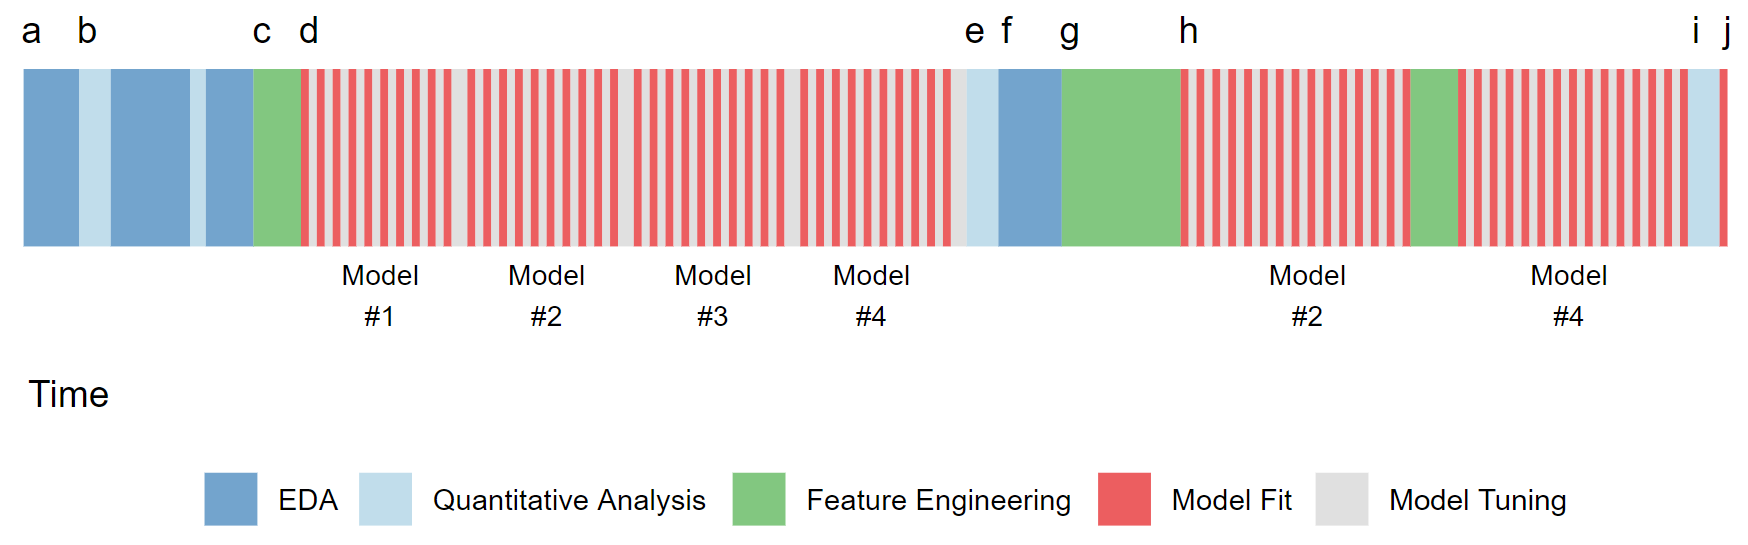
\includegraphics{Images/modelling-process.png}

\hypertarget{cac-nhom-thut-ng-cn-nh}{%
\section{Các nhóm thuật ngữ cần nhớ}\label{cac-nhom-thut-ng-cn-nh}}

\begin{itemize}
\tightlist
\item
  \textbf{Độ biến động (variance)} vs. \textbf{độ chuẩn xác (bias)}:

  \begin{itemize}
  \tightlist
  \item
    \texttt{variance} là độ biến động của mô hình so với dữ liệu, đo độ
    nhạy cảm của các tham số trong mô hình khi thay đổi dữ liệu. Nói
    cách khác, một mô hình được gọi là biến động lớn khi dữ liệu mô hình
    thay đổi sẽ dẫn đến một sự thay đổi lớn trong mô hình. Ví dụ, mô
    hình sử dụng trung vị làm biến dự báo sẽ ít biến động hơn khi sử
    dụng giá trị trung bình.
  \item
    \texttt{bias} đo độ \texttt{chuẩn\ xác} của mô hình. Một mô hình
    được gọi là \texttt{bias} thấp khi kết quả dự báo gần với kết quả
    thực tế và ngược lại. Các mô hình có \texttt{bias} thấp có khả năng
    thích ứng với dữ liệu tốt, các mô hình như cây quyết đinh, neural
    network thuộc dạng này.
  \end{itemize}
\end{itemize}

\hypertarget{luu-y}{%
\section{Lưu ý}\label{luu-y}}

\begin{itemize}
\tightlist
\item
  Khi xây dựng mô hình, hiệu ứng của các biến dự báo (predictor) có thể
  lớn hơn thuật toán rất nhiều
\item
  Với cùng một nhóm các biến dự báo đúng thực tế, các thuật toán khác
  nhau có thể đưa ra các kết quả tương tự nhau.
\end{itemize}

\mainmatter

\hypertarget{feature-engineering}{%
\chapter{Feature Engineering}\label{feature-engineering}}

Khi xây dựng mô hình dự báo, ta phải cân bằng giữa độ chính xác và khả
năng giải thích của mô hình. Trong nhiều trường hợp, khả năng giải thích
được ưu tiên hơn, thể hiện rất rõ trong các mô hình score card của rủi
ro trong hệ thống ngân hàng. Tuy nhiên, ta không thể hy sinh độ chính
xác để lấy khả năng giải thích nếu độ chính xác của mô hình không đạt
đến một ngưỡng nhất định. Khi đó, có hai cách tiếp cận:

\begin{itemize}
\tightlist
\item
  Cho thêm biến vào mô hình.
\item
  Thay đổi các biến có sẵn bằng các nhóm biến phái sinh để mô hình tốt
  hơn - cách tiếp cận này gọi là \texttt{feature\ engineering}.
\end{itemize}

\texttt{Feature\ Engineering} là quá trình thể hiện các biến đầu vào
(variables) với những cách thức khác nhau để giúp cho tăng độ chính xác
của mô hình dự báo. Ví dụ:

\begin{itemize}
\tightlist
\item
  Địa điểm của khách hàng có thể được thể hiện bằng ZIP code hoặc cùng
  lúc 2 biến, kinh độ và vĩ độ.
\item
  Biến dự báo \texttt{age} có thể cho ra kết quả tốt hơn trong mô hình
  khi ta dùng biến \(\frac{1}{age}\)
\end{itemize}

Với mỗi mô hình, thuật toán khác nhau sẽ yêu cầu những cách thức triển
khai và thay đổi biến đầu vào khác nhau. Do đó, khi lựa chọn cách thức
biến đổi biến đầu vào, ta phải nắm rất rõ thuật toán và cách thức biến
đổi dữ liệu theo từng trường hợp khác nhau. Đối với
\texttt{feature\ engineering}, ta có thể chia làm 2 nhóm chính.

\begin{itemize}
\tightlist
\item
  Biến đổi các biến định dạng nhóm (categorical)
\item
  Biến đổi các biến định dạng số (numeric)
\end{itemize}

\hypertarget{feature-engineering-cho-cac-bin-nhom}{%
\section{Feature engineering cho các biến
nhóm}\label{feature-engineering-cho-cac-bin-nhom}}

\hypertarget{tao-d-liu-gia-dummy-data-cho-bin-khong-phan-bit-th-t}{%
\subsection{Tạo dữ liệu giả (dummy data) cho biến không phân biệt thứ
tự}\label{tao-d-liu-gia-dummy-data-cho-bin-khong-phan-bit-th-t}}

Trong phương pháp này, toàn bộ các dữ liệu gốc được chuyển sang dạng
0-1. Tuy nhiên, dữ liệu mới được tạo ra sẽ ít hơn dữ liệu gốc 1 trường
hợp. Bởi lẽ khi biết giá trị của 6 biến, ta có thể biết được giá trị của
biến cuối cùng.

\begin{longtable}[]{@{}lllllll@{}}
\toprule
Biến gốc & Mon & Tues & Wed & Thurs & Fri & Sat\tabularnewline
\midrule
\endhead
Sun & 0 & 0 & 0 & 0 & 0 & 0\tabularnewline
Mon & 1 & 0 & 0 & 0 & 0 & 0\tabularnewline
Tues & 0 & 1 & 0 & 0 & 0 & 0\tabularnewline
Wed & 0 & 0 & 1 & 0 & 0 & 0\tabularnewline
Thurs & 0 & 0 & 0 & 1 & 0 & 0\tabularnewline
Fri & 0 & 0 & 0 & 0 & 1 & 0\tabularnewline
Sat & 0 & 0 & 0 & 0 & 0 & 1\tabularnewline
\bottomrule
\end{longtable}

\textbf{zero-variance predictor}: là biến chỉ có một giá trị. Khi xây
dựng mô hình, ta cần loại biến này.

\hypertarget{d-liu-co-rt-nhiu-nhom}{%
\subsection{Dữ liệu có rất nhiều nhóm}\label{d-liu-co-rt-nhiu-nhom}}

Đối với các biến có rất nhiều nhóm (ví dụ: 200 chi nhánh trong ngân
hàng), ta có 2 cách tiếp cận.

\begin{itemize}
\tightlist
\item
  Cách một, dựa vào kiến thức nghiệp vụ tự nhóm. Ví dụ, các chi nhánh ở
  Hà Nội sẽ đánh dấu là HN, ở Hồ Chí Minh là HCM, các chi nhánh còn lại
  là \texttt{Others}.
\item
  Cách hai, sử dụng \texttt{hash\ function}. Trong trường hợp này, các
  biến category sẽ được tạo thành một biến hoàn toàn mới có giá trị số.
  Xem ví dụ dưới đây.
\end{itemize}

\begin{longtable}[]{@{}ll@{}}
\toprule
Giá trị & Hash\tabularnewline
\midrule
\endhead
belvedere tiburon & 582753783\tabularnewline
berkeley & 1166288024\tabularnewline
\bottomrule
\end{longtable}

\textbf{Lưu ý}: Nhiều thí nghiệm đã được sử dụng để so sánh sự khác biệt
giữa việc dùng factor và encoding 0-1 trong dữ liệu. Kết quả cho thấy
không có nhiều sự khác biệt giữa hai cách.

\hypertarget{cac-bin-lien-tuc}{%
\section{Các biến liên tục}\label{cac-bin-lien-tuc}}

Đối với các biến liên tục, khi xây dựng mô hình, ta sẽ gặp phải các vấn
đề sau.

\begin{itemize}
\tightlist
\item
  Các biến có các đơn vị khác nhau. Ví dụ, tuổi có giá trị từ 15-75, thu
  nhập có giá trị từ 2 triệu VND đến 200 triệu VND
\item
  Các biến bị lệch sang phải (skewness)
\item
  Các biến có xuất hiện giá trị ngoại lai (outliers)
\item
  Các biến có thể bị chặn trai hoặc chặn phải. Ví dụ, độ tuổi có giá trị
  không quá 80
\end{itemize}

Đối với các biến số, có ba nhóm kỹ thuật lớn biến đổi dữ liệu.

\begin{itemize}
\tightlist
\item
  Biến đổi 1:1 - một biến được biến đổi thành một biến khác
\item
  Biến đổi 1:n - một biến được biến đổi thành nhiều biến khác nhau
\item
  Biến đổi n:n - n biến gốc được biến đổi cùng lúc thành n biến khác
\end{itemize}

\hypertarget{bin-i-11}{%
\subsection{Biến đổi 1:1}\label{bin-i-11}}

Trong biến đổi 1:1, có rất nhiều cách khác nhau.

\begin{itemize}
\tightlist
\item
  Biến đổi theo scale của dữ liệu: log, Box-Cox
\end{itemize}

\[x^{*} = \left\{ \begin{array}{l l} \frac{x^{\lambda}-1}{\lambda\: \tilde{x}^{\lambda-1}}, & \lambda \neq 0 \\ \tilde{x} \: \log x, & \lambda = 0 \\ \end{array} \right.\]

\mainmatter

\hypertarget{part-chui-thi-gian}{%
\part{Chuỗi thời gian}\label{part-chui-thi-gian}}

\hypertarget{gii-thiu-v-chui-thi-gian}{%
\chapter{Giới thiệu về chuỗi thời gian}\label{gii-thiu-v-chui-thi-gian}}

Khi phân tích dữ liệu, có hai khái niệm đều được gọi là \emph{dự báo}
khi được dịch sang tiếng Việt, đó là \texttt{forcast} và
\texttt{predict}. Tuy nhiên, hai khái niệm này rất khác nhau.

\begin{itemize}
\tightlist
\item
  \textbf{Predict}: Thường được dùng để chỉ việc dự báo xác suất xảy ra
  các sự kiện. Ví dụ, xác suất vỡ nợ, xác suất khách hàng churn,\ldots{}
\item
  \textbf{Forecast}: Thường dùng trong việc dự báo chuỗi thời gian. Ví
  dụ, dựa vào lịch sử biến động của tổng khách hàng uống cafe theo tuần,
  ta có thể \emph{dự báo} được số lượng khách hàng uống cafe của 1 tuần
  tới, hai tuần tới,\ldots{}
\end{itemize}

Trong phần trước, chúng ta đã bàn nhiều về nhóm \texttt{predict}, trong
phần này, ta sẽ bàn thêm về nhóm \texttt{forecast}, về các cấu phần và
cách thức dự báo đối với chuỗi thời gian. Do đó, trong phần này, khi nói
về dự báo, chúng ta đang bàn về vấn đề \texttt{forecast}.

\textbf{Phân biệt \texttt{dự\ báo}, \texttt{mục\ tiêu} và
\texttt{kế\ hoạch}}

\textbf{Dự báo}: là quá trình sử dụng các thông tin hiện hữu đưa ra các
nhận định chính xác nhất có thể có trong tương lai trong một khoảng thời
gian xác định về một chỉ số nào đó.

\textbf{Mục tiêu}: là thứ mà cá nhân, tổ chức mong muốn đạt được trong
một khoảng thời gian xác định trong tương lai. Thường thì mục tiêu được
đặt mà không quan tâm đến bất kỳ đến việc dự báo nào cả. Ví dụ, mục tiêu
tăng trưởng của doanh nghiệp thường là năm sau cao gấp đôi năm trước
trong khi dự báo chỉ có thể tăng được 30\%.

\textbf{Kế hoạch}: Là phản ứng của tổ chức, cá nhân đối với \emph{dự
báo} và \emph{mục tiêu}. Việc lập kế hoạch đòi hỏi nhiều hành động cụ
thể để điều hướng dự báo sát sát với mục tiêu (hoặc vượt mục tiêu)

Xét về yếu tố thời gian, việc dự báo có thể chia thành dự báo ngắn hạn,
trung hạn và dài hạn.

\textbf{Các điểm khi dự báo}

Khi dự báo, có hai điểm quan trọng chúng ta phải trả lời.

\begin{itemize}
\tightlist
\item
  Thứ nhất, ta cần dự báo điều gì? Dự báo với từng sản phẩm hay với cả
  nhóm sản phẩm? Dự báo doanh số bán hàng của từng cửa hàng hay của toàn
  hệ thống?
\item
  Thứ hai, yếu tố thời gian xét trong vấn đề dự báo này là gì? Ta cần dự
  báo trong bao lâu? Tần xuất như thế nào? Ví dụ, dư báo doanh số bán
  hàng mỗi tháng/tuần 1 lần trong 1 năm tới?
\end{itemize}

\begin{quote}
\textbf{Lưu ý}: Các bạn phân tích dữ liệu cần phải tìm hiểu các đơn vị
nghiệp vụ sẽ sử dụng kết quả dự báo như thế nào, để tránh việc bỏ quá
nhiều thời gian và công sức dự báo nhưng không ai sử dụng.
\end{quote}

\hypertarget{thanh-phn-cua-chui-thi-gian}{%
\section{Thành phần của chuỗi thời
gian}\label{thanh-phn-cua-chui-thi-gian}}

Trong bất cứ chuỗi thời gian nào, cũng có 3 thành phần sau.

\begin{itemize}
\tightlist
\item
  \textbf{Xu hướng} (trend) thể hiện chiều hướng tăng hay giảm dài hạn
  của chuỗi thời gian
\item
  \textbf{Mùa vụ} (seasonal) thể hiện sự biến đổi của chuỗi thời gian
  theo chu kỳ biết trước. Ví dụ, vào cuối tuần, khách hàng có xu hướng
  đi ăn nhà hàng nhiều hơn.
\item
  \textbf{Chu kỳ kinh doanh} (cyclic) thể hiện xu hướng biến đổi dài hạn
  của chuỗi thời gian, thường ít nhất hai năm. Chu kỳ kinh doanh khác
  với yếu tố mùa vụ ở chỗ, chu kỳ biến đổi của yếu tố mùa vụ thường là
  đã được biết trước và mang tính ngắn hạn.
\end{itemize}

\mainmatter

\hypertarget{part-case-study}{%
\part{Case study}\label{part-case-study}}

Quá trình phân tích dữ liệu không phải chỉ là việc áp dụng lý thuyết một
cách máy móc và đòi hỏi sự sáng tạo và linh hoạt trong từng trường hợp
cụ thể và rất khác nhau trong từng lĩnh vực. Ở phần này, tác giả sẽ
trình bày các ứng dụng thực tiễn theo nhiều lĩnh vực khác nhau,

\hypertarget{trc-quan-hoa-d-liu}{%
\chapter{Trực quan hóa dữ liệu}\label{trc-quan-hoa-d-liu}}

\hypertarget{xay-dng-phu-ban-hang-theo-tng-nhom}{%
\section{Xây dựng phễu bán hàng theo từng
nhóm}\label{xay-dng-phu-ban-hang-theo-tng-nhom}}

Trong quá trình phân tích bán hàng, phếu bán hàng (sale funnel) là một
kỹ thuật rất hữu dụng để trực quan hóa kết quả kinh doanh theo từng
nhóm. Tuy nhiên, hiện ít có biểu đồ nào thể hiện được phễu bán hàng một
cách hiệu quả trên R.

Trong mục này, tác giả sẽ hướng dẫn một ví dụ thực tiễn trực quan hóa
phễu bán hàng một cách hiệu quả.

Xem ví dụ điển hình về phễu bán hàng dưới đây

\begin{Shaded}
\begin{Highlighting}[]
\NormalTok{data <-}\StringTok{ }\KeywordTok{read.table}\NormalTok{(}\KeywordTok{textConnection}\NormalTok{(}
          \KeywordTok{c}\NormalTok{(}\StringTok{"step;segment1;segment2;segment3;total}
\StringTok{          1_visit;1806;11663;12641;26110}
\StringTok{          2_register;1143;6476;5372;12991}
\StringTok{          3_login;1806;11663;2694;16163}
\StringTok{          4_subscribe;21;3322;2694;6037}
\StringTok{          5_paid;259;422;41;722"}\NormalTok{)),}
        \DataTypeTok{header =}\NormalTok{ T, }\DataTypeTok{sep =} \StringTok{";"}\NormalTok{)}
\CommentTok{# Dữ liệu}
\NormalTok{data}
\end{Highlighting}
\end{Shaded}

\begin{verbatim}
##                    step segment1 segment2 segment3
## 1               1_visit     1806    11663    12641
## 2            2_register     1143     6476     5372
## 3               3_login     1806    11663     2694
## 4           4_subscribe       21     3322     2694
## 5                5_paid      259      422       41
##   total
## 1 26110
## 2 12991
## 3 16163
## 4  6037
## 5   722
\end{verbatim}

Trong tập dữ liệu trên, ta sẽ mô phỏng dữ liệu phếu bán hàng của 3 phân
khúc khách hàng trên một trang thương mại điện tử mà trong đó, khách
hàng sẽ đi qua năm bước khác nhau:

\begin{itemize}
\tightlist
\item
  Ghé thăm website (visit)
\item
  Đăng ký (register)
\item
  Đăng nhập (login)
\item
  Đăng ký cập nhật các thông tin sản phẩm (subscribe)
\item
  Mua hàng và trả tiền thành công (paid)
\end{itemize}

Để tạo một biểu đồ phễu bán hàng, ta sẽ thực hiện 3 bước lớn sau.

\begin{itemize}
\tightlist
\item
  Tạo \texttt{theme} cho biểu đồ
\item
  Tạo các biểu đồ con cho phễu bán hàng
\item
  Kết hợp các biểu đồ để tạo thành phễu bán hàng hoàn chỉnh
\end{itemize}

\begin{Shaded}
\begin{Highlighting}[]
\CommentTok{# Gọi library}
\KeywordTok{library}\NormalTok{(tidyverse)}
\KeywordTok{library}\NormalTok{(reshape2)}
\KeywordTok{library}\NormalTok{(forcats)}
\KeywordTok{library}\NormalTok{(ggthemes)}

\CommentTok{# Tạo theme trông cho chart}
\NormalTok{funnel_theme <-}\StringTok{ }\KeywordTok{theme}\NormalTok{(}\DataTypeTok{axis.title =} \KeywordTok{element_blank}\NormalTok{(),}
        \DataTypeTok{axis.ticks.x =} \KeywordTok{element_blank}\NormalTok{(),}
        \DataTypeTok{axis.text.x =} \KeywordTok{element_blank}\NormalTok{(),}
        \DataTypeTok{legend.position =} \StringTok{"none"}\NormalTok{,}
        \DataTypeTok{panel.grid =} \KeywordTok{element_blank}\NormalTok{()}
\NormalTok{        )}

\CommentTok{# Phân rã dữ liệu}
\NormalTok{df <-}\StringTok{ }\NormalTok{data }\OperatorTok\StringTok{ }\KeywordTok{melt}\NormalTok{(}\DataTypeTok{id.vars =} \StringTok{"step"}\NormalTok{)}

\CommentTok{# Tạo biểu đồ chính}
\NormalTok{p1 <-}\StringTok{ }\NormalTok{df }\OperatorTok\StringTok{ }
\StringTok{  }\KeywordTok{mutate}\NormalTok{(}\DataTypeTok{step =} \KeywordTok{fct_rev}\NormalTok{(step)) }\OperatorTok\StringTok{ }
\StringTok{  }\KeywordTok{filter}\NormalTok{(variable }\OperatorTok{!=}\StringTok{ "total"}\NormalTok{) }\OperatorTok\StringTok{ }
\StringTok{  }\KeywordTok{ggplot}\NormalTok{(}\KeywordTok{aes}\NormalTok{(step, value)) }\OperatorTok{+}
\StringTok{  }\KeywordTok{geom_bar}\NormalTok{(}\KeywordTok{aes}\NormalTok{(}\DataTypeTok{fill =}\NormalTok{ variable), }\DataTypeTok{stat =} \StringTok{"identity"}\NormalTok{) }\OperatorTok{+}
\StringTok{  }\KeywordTok{facet_grid}\NormalTok{(}\OperatorTok{~}\NormalTok{variable, }\DataTypeTok{scale =} \StringTok{"free"}\NormalTok{) }\OperatorTok{+}
\StringTok{  }\KeywordTok{coord_flip}\NormalTok{() }\OperatorTok{+}\StringTok{ }
\StringTok{  }\KeywordTok{geom_text}\NormalTok{(}\KeywordTok{aes}\NormalTok{(}\DataTypeTok{label =}\NormalTok{ value),}
            \DataTypeTok{position =} \KeywordTok{position_stack}\NormalTok{(}\DataTypeTok{vjust =} \FloatTok{.5}\NormalTok{)) }\OperatorTok{+}
\StringTok{  }\KeywordTok{scale_fill_tableau}\NormalTok{() }\OperatorTok{+}
\StringTok{  }\KeywordTok{theme_minimal}\NormalTok{() }\OperatorTok{+}
\StringTok{  }\KeywordTok{scale_y_sqrt}\NormalTok{() }\OperatorTok{+}
\StringTok{  }\NormalTok{funnel_theme }\OperatorTok{+}
\StringTok{  }\KeywordTok{theme}\NormalTok{(}\DataTypeTok{plot.margin=}\NormalTok{grid}\OperatorTok{::}\KeywordTok{unit}\NormalTok{(}\KeywordTok{c}\NormalTok{(}\DecValTok{0}\NormalTok{,}\DecValTok{0}\NormalTok{,}\DecValTok{0}\NormalTok{,}\DecValTok{0}\NormalTok{), }\StringTok{"mm"}\NormalTok{)) }\OperatorTok{+}
\StringTok{  }\KeywordTok{theme}\NormalTok{(}
  \DataTypeTok{axis.text.y =} \KeywordTok{element_blank}\NormalTok{(),}
  \DataTypeTok{strip.text =} \KeywordTok{element_text}\NormalTok{(}\DataTypeTok{size =} \DecValTok{14}\NormalTok{, }
                            \DataTypeTok{face =} \StringTok{"bold"}\NormalTok{)) }\OperatorTok{+}
\StringTok{  }\KeywordTok{theme}\NormalTok{(}
    \DataTypeTok{panel.spacing =} \KeywordTok{unit}\NormalTok{(}\DecValTok{0}\NormalTok{, }\StringTok{"mm"}\NormalTok{)) }\OperatorTok{+}
\StringTok{  }\KeywordTok{annotate}\NormalTok{(}\StringTok{"rect"}\NormalTok{, }\DataTypeTok{xmin =} \FloatTok{0.5}\NormalTok{, }\DataTypeTok{xmax =} \FloatTok{1.5}\NormalTok{, }\DataTypeTok{ymin =} \DecValTok{0}\NormalTok{, }\DataTypeTok{ymax =} \OtherTok{Inf}\NormalTok{,}
           \DataTypeTok{alpha =} \FloatTok{.2}\NormalTok{) }\OperatorTok{+}
\StringTok{  }\KeywordTok{annotate}\NormalTok{(}\StringTok{"rect"}\NormalTok{, }\DataTypeTok{xmin =} \FloatTok{2.5}\NormalTok{, }\DataTypeTok{xmax =} \FloatTok{3.5}\NormalTok{, }\DataTypeTok{ymin =} \DecValTok{0}\NormalTok{, }\DataTypeTok{ymax =} \OtherTok{Inf}\NormalTok{,}
           \DataTypeTok{alpha =} \FloatTok{.2}\NormalTok{) }\OperatorTok{+}
\StringTok{  }\KeywordTok{annotate}\NormalTok{(}\StringTok{"rect"}\NormalTok{, }\DataTypeTok{xmin =} \FloatTok{4.5}\NormalTok{, }\DataTypeTok{xmax =} \FloatTok{5.5}\NormalTok{, }\DataTypeTok{ymin =} \DecValTok{0}\NormalTok{, }\DataTypeTok{ymax =} \OtherTok{Inf}\NormalTok{,}
           \DataTypeTok{alpha =} \FloatTok{.2}\NormalTok{) }\OperatorTok{+}
\StringTok{  }\KeywordTok{theme}\NormalTok{(}\DataTypeTok{axis.text.y =} \KeywordTok{element_blank}\NormalTok{())}
\NormalTok{p1}
\end{Highlighting}
\end{Shaded}

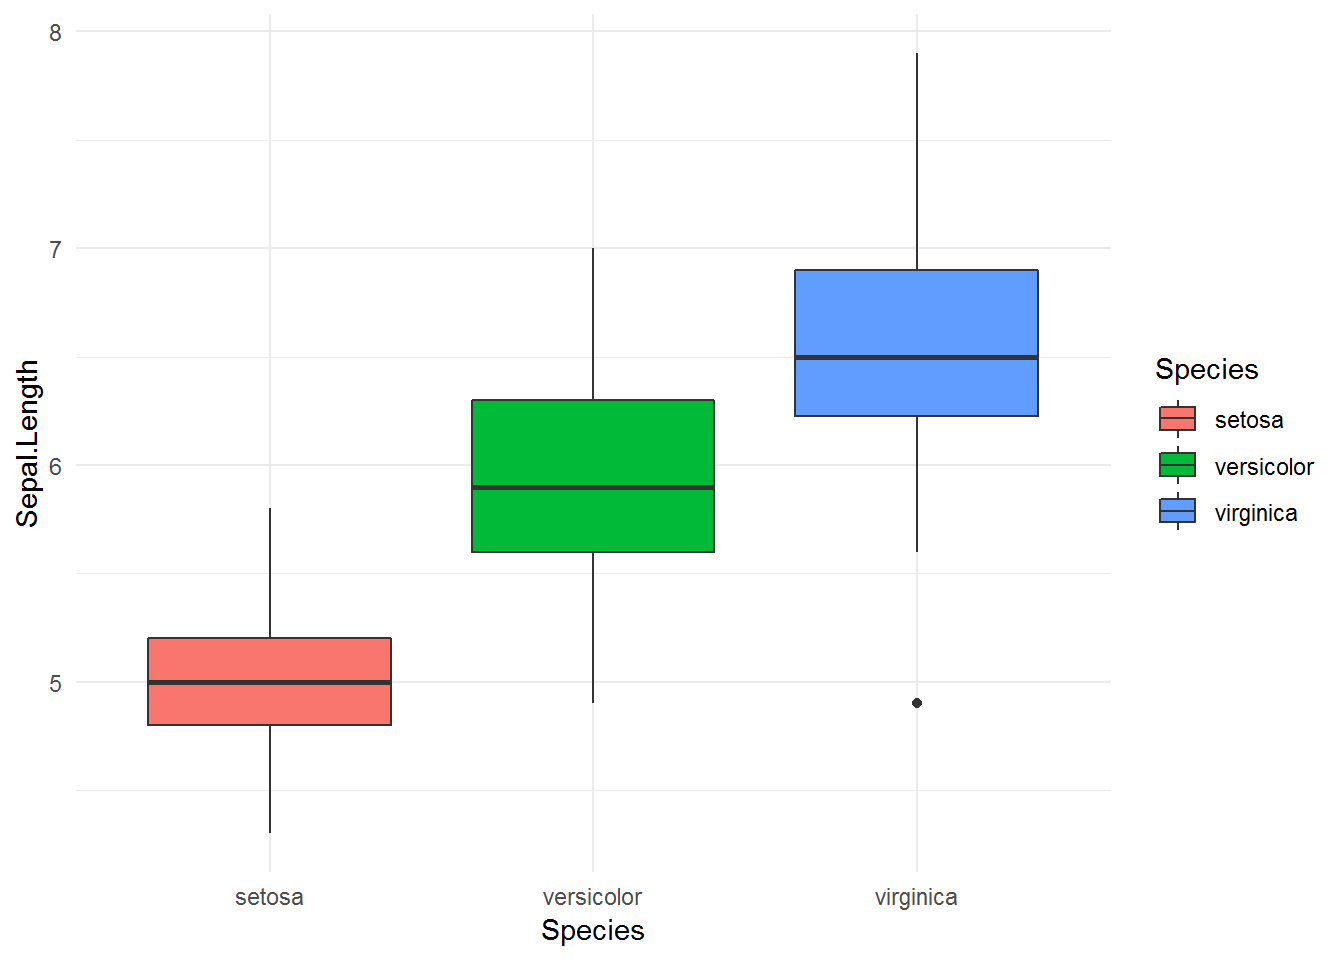
\includegraphics{bookdown_files/figure-latex/unnamed-chunk-61-1.pdf}

\begin{itemize}
\tightlist
\item
  Tạo thêm phần \texttt{label} tổng theo từng segment
\end{itemize}

\begin{Shaded}
\begin{Highlighting}[]
\NormalTok{df }\OperatorTok
\StringTok{  }\KeywordTok{mutate}\NormalTok{(}\DataTypeTok{step =} \KeywordTok{fct_rev}\NormalTok{(step)) }\OperatorTok
\StringTok{  }\KeywordTok{filter}\NormalTok{(variable }\OperatorTok{==}\StringTok{ "total"}\NormalTok{) }\OperatorTok
\StringTok{  }\KeywordTok{ggplot}\NormalTok{(}\KeywordTok{aes}\NormalTok{(step, }\DecValTok{0}\NormalTok{)) }\OperatorTok{+}
\StringTok{  }\KeywordTok{geom_label}\NormalTok{(}\KeywordTok{aes}\NormalTok{(}\DataTypeTok{label =}\NormalTok{ value),}
             \DataTypeTok{col =} \StringTok{"white"}\NormalTok{,}
             \DataTypeTok{fill =} \StringTok{"darkred"}\NormalTok{,}
             \DataTypeTok{size =} \DecValTok{4}\NormalTok{) }\OperatorTok{+}
\StringTok{  }\KeywordTok{coord_flip}\NormalTok{() }\OperatorTok{+}
\StringTok{  }\KeywordTok{facet_wrap}\NormalTok{(}\OperatorTok{~}\NormalTok{variable) }\OperatorTok{+}
\StringTok{  }\KeywordTok{theme_minimal}\NormalTok{() }\OperatorTok{+}
\StringTok{  }\KeywordTok{theme}\NormalTok{(}\DataTypeTok{axis.text =} \KeywordTok{element_blank}\NormalTok{()) }\OperatorTok{+}
\StringTok{  }\NormalTok{funnel_theme }\OperatorTok{+}
\StringTok{  }\KeywordTok{theme}\NormalTok{(}
    \DataTypeTok{strip.text.x =} \KeywordTok{element_blank}\NormalTok{()}
\NormalTok{  ) ->}\StringTok{ }\NormalTok{p2}
\NormalTok{p2}
\end{Highlighting}
\end{Shaded}

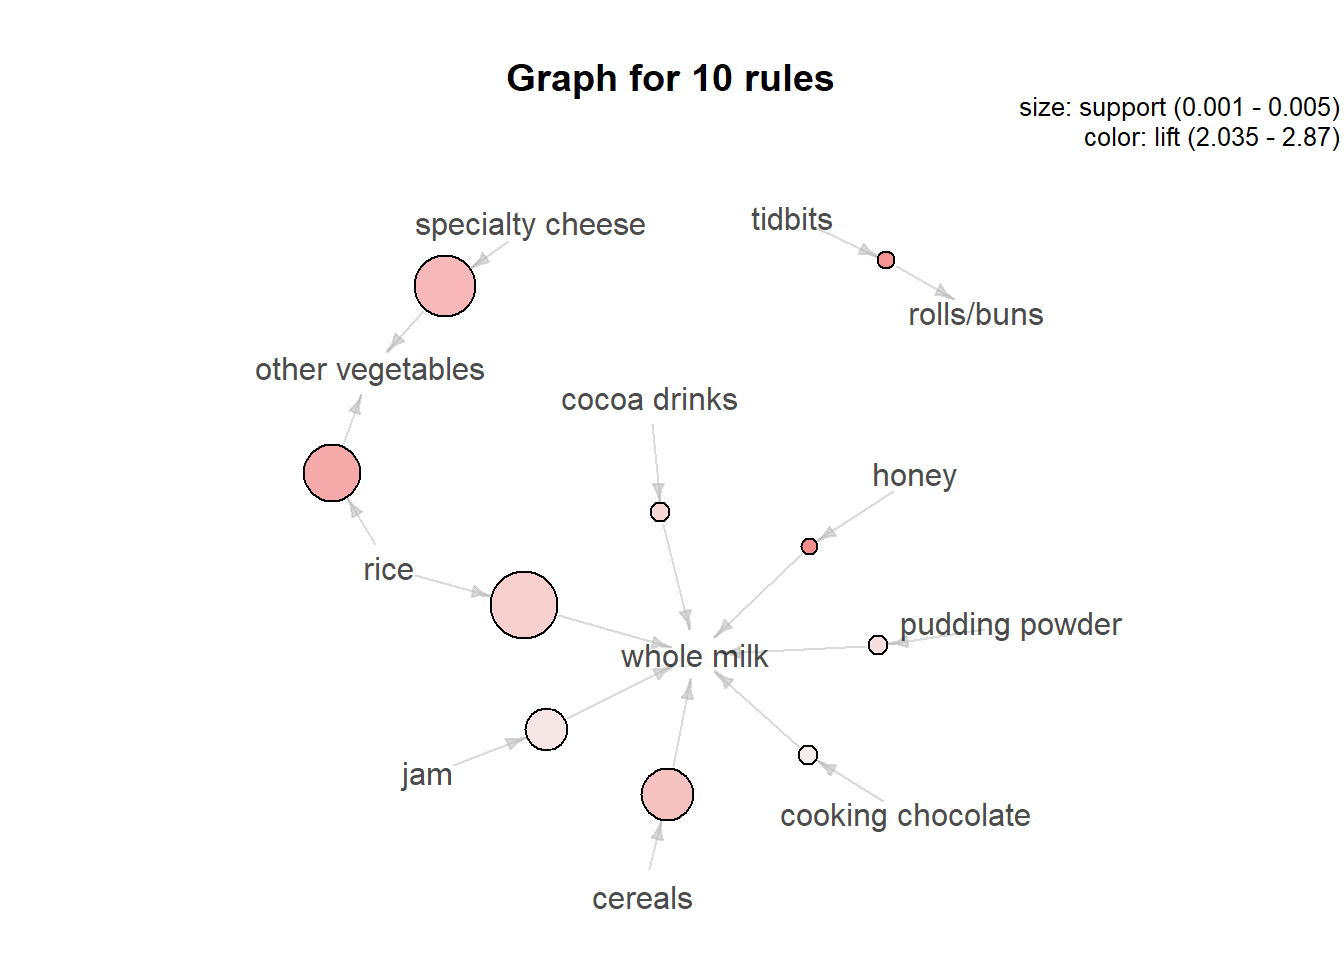
\includegraphics{bookdown_files/figure-latex/unnamed-chunk-62-1.pdf}

\begin{itemize}
\tightlist
\item
  Tạo thêm thứ tự các bước trong phễu bán hàng để dễ theo dõi hơn
\end{itemize}

\begin{Shaded}
\begin{Highlighting}[]
\NormalTok{df2 <-}\StringTok{ }\KeywordTok{data.frame}\NormalTok{(}\DataTypeTok{step =}\NormalTok{ data}\OperatorTok{$}\NormalTok{step,}
                  \DataTypeTok{value =} \DecValTok{1}\OperatorTok{:}\DecValTok{5}\NormalTok{)}
\NormalTok{df2 }\OperatorTok\StringTok{ }
\StringTok{  }\KeywordTok{mutate}\NormalTok{(}\DataTypeTok{step =} \KeywordTok{fct_rev}\NormalTok{(step)) }\OperatorTok\StringTok{ }
\StringTok{  }\KeywordTok{ggplot}\NormalTok{(}\KeywordTok{aes}\NormalTok{(step, }\DecValTok{1}\NormalTok{)) }\OperatorTok{+}
\StringTok{  }\KeywordTok{geom_hline}\NormalTok{(}\DataTypeTok{yintercept =} \DecValTok{1}\NormalTok{) }\OperatorTok{+}
\StringTok{  }\KeywordTok{geom_point}\NormalTok{(}\DataTypeTok{size =} \DecValTok{10}\NormalTok{, }\DataTypeTok{col =} \StringTok{"darkgreen"}\NormalTok{) }\OperatorTok{+}
\StringTok{  }\KeywordTok{geom_text}\NormalTok{(}\KeywordTok{aes}\NormalTok{(}\DataTypeTok{label =}\NormalTok{ value), }
            \DataTypeTok{col =} \StringTok{"white"}\NormalTok{) }\OperatorTok{+}
\StringTok{  }\KeywordTok{coord_flip}\NormalTok{() }\OperatorTok{+}
\StringTok{  }\KeywordTok{theme_minimal}\NormalTok{() }\OperatorTok{+}
\StringTok{  }\NormalTok{funnel_theme }\OperatorTok{+}
\StringTok{  }\KeywordTok{theme}\NormalTok{(}
    \DataTypeTok{axis.text =} \KeywordTok{element_text}\NormalTok{(}\DataTypeTok{size =} \DecValTok{14}\NormalTok{)}
\NormalTok{  ) ->}\StringTok{ }\NormalTok{p3}
\NormalTok{p3}
\end{Highlighting}
\end{Shaded}

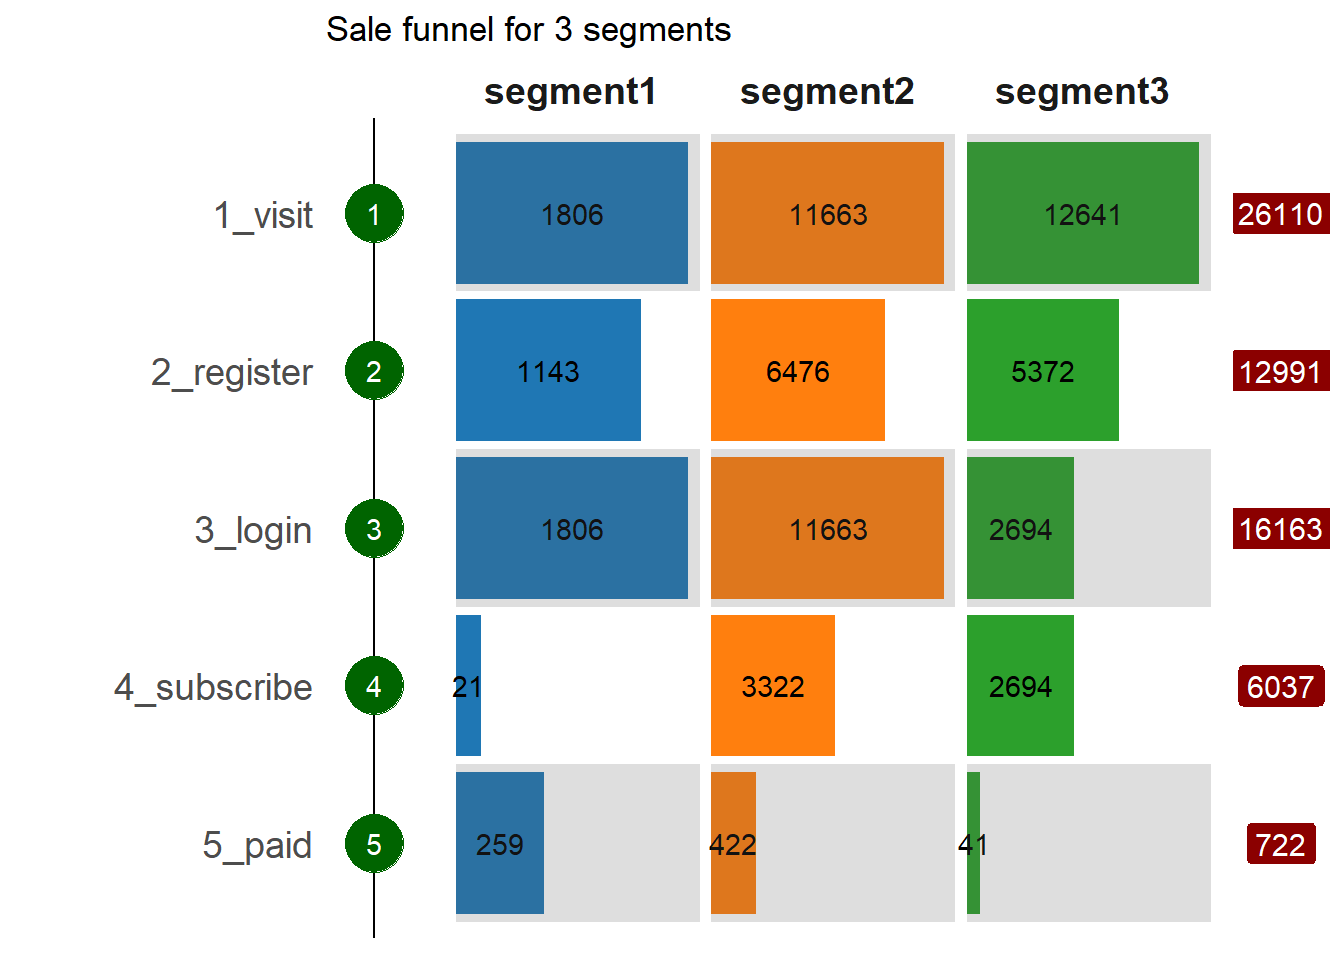
\includegraphics{bookdown_files/figure-latex/unnamed-chunk-63-1.pdf}

\begin{itemize}
\tightlist
\item
  Cuối cùng, ta có thể tạo ghép các biểu đồ rời rạc để tạo thành phễu
  bán hàng hoàn chỉnh. Việc kết hợp các biểu đồ trên \texttt{ggplot2} có
  thể hoàn thành một cách đơn giản với \texttt{ggplot2}
\end{itemize}

\begin{Shaded}
\begin{Highlighting}[]
\CommentTok{#devtools::install_github("thomasp85/patchwork")}
\KeywordTok{library}\NormalTok{(patchwork)}
\NormalTok{p3 }\OperatorTok{+}\StringTok{ }
\StringTok{  }\KeywordTok{labs}\NormalTok{(}\DataTypeTok{title =} \StringTok{"Sale funnel for 3 segments"}\NormalTok{) }\OperatorTok{+}
\StringTok{  }\NormalTok{p1 }\OperatorTok{+}\StringTok{ }\NormalTok{p2 }\OperatorTok{+}\StringTok{ }
\StringTok{  }\KeywordTok{plot_layout}\NormalTok{(}\DataTypeTok{nrow =} \DecValTok{1}\NormalTok{, }\DataTypeTok{widths =} \KeywordTok{c}\NormalTok{(}\DecValTok{1}\NormalTok{, }\DecValTok{8}\NormalTok{, }\DecValTok{1}\NormalTok{))}
\end{Highlighting}
\end{Shaded}

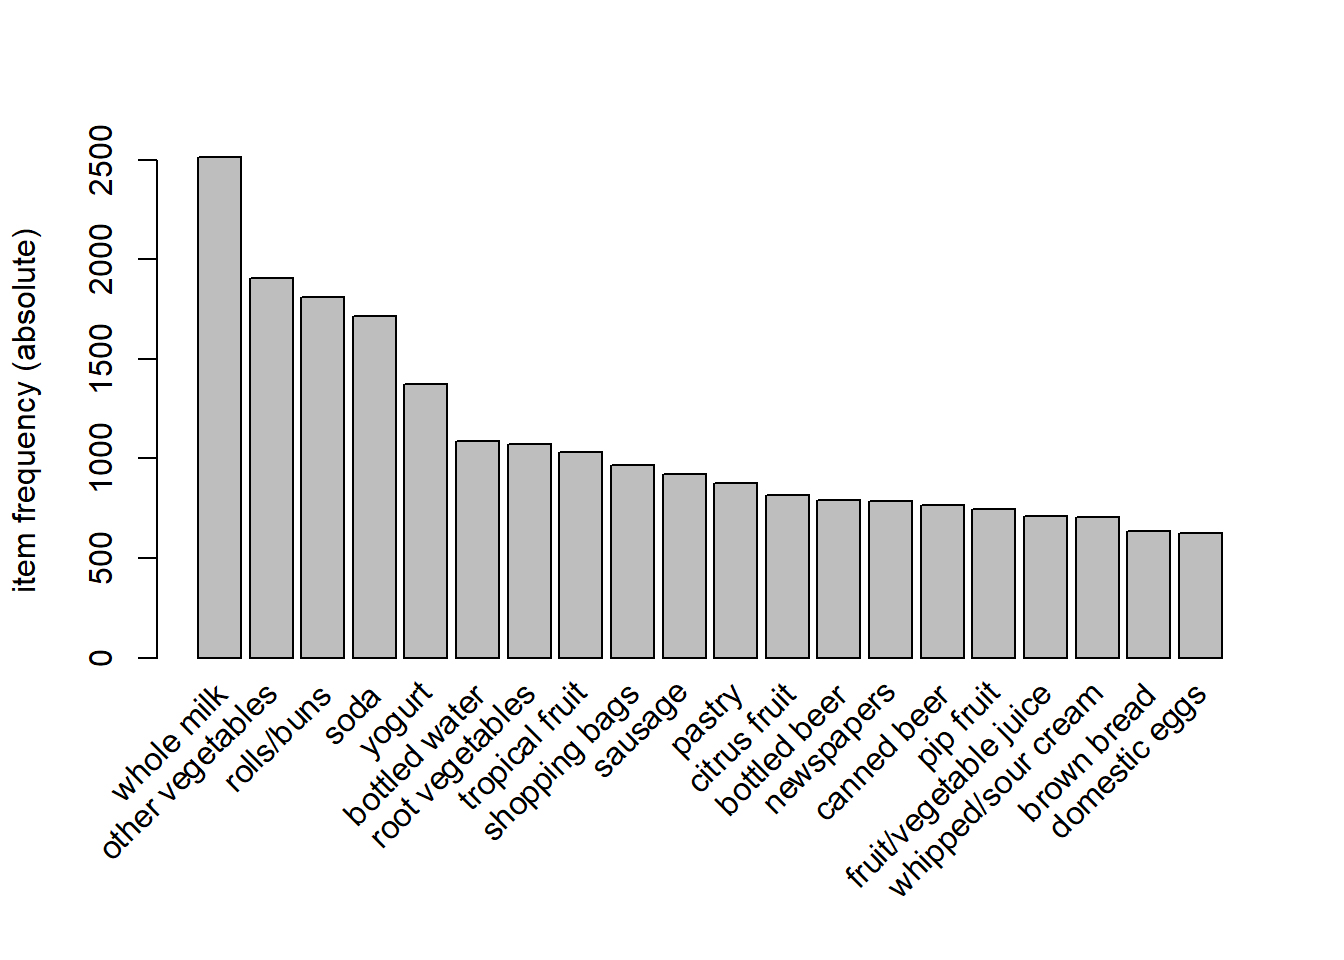
\includegraphics{bookdown_files/figure-latex/unnamed-chunk-64-1.pdf}

Như vậy, chúng ta đã hoàn thành phễu bán hàng rất chuyên nghiệp với
\texttt{ggplot2}. Phễu bán hàng này đặc biệt hiệu quả khi cùng lúc phải
so sánh nhiều phân khúc khách hàng khác nhau trên toàn bộ chuỗi bán
hàng.

\hypertarget{ve-biu--warterfall-cho-aciveinactive-users}{%
\section{Vẽ biểu đồ warterfall cho acive/inactive
users}\label{ve-biu--warterfall-cho-aciveinactive-users}}

Trong kỷ nguyên số, chỉ số \texttt{active\ user} (tạm dịch: người dùng
thường xuyên hoạt động) là chỉ số đặc biệt quan trọng với bất kỳ
website/ app nào. Công thức tính chỉ số người dùng thường xuyên hoạt
động tại khoảng thời gian \emph{t} được tính như sau:

\[active_{t} = active_{t-1} + new_{t} - churn_{t}\]

Ví dụ về waterfall chart được lấy từ ví dụ của Tableau tại đường link:
{[}\url{https://public.tableau.com/views/CH24_BBOD_ChurnTurnover/SubscriberChurnAnalysis}{]}

Trong case study này, chúng ta sẽ tìm cách xây dựng một biểu đồ
waterfall chart tương tự

\begin{Shaded}
\begin{Highlighting}[]
\CommentTok{# Load library}
\KeywordTok{library}\NormalTok{(tidyverse)}
\KeywordTok{library}\NormalTok{(ggplot2)}
\KeywordTok{library}\NormalTok{(reshape2)}
\KeywordTok{library}\NormalTok{(lubridate)}
\KeywordTok{library}\NormalTok{(grid)}
\KeywordTok{library}\NormalTok{(gridExtra)}

\CommentTok{# Tạo dữ liệu giả lập}
\KeywordTok{set.seed}\NormalTok{(}\DecValTok{123}\NormalTok{)}
\NormalTok{data <-}\StringTok{ }\KeywordTok{data.frame}\NormalTok{(}\DataTypeTok{date =} \KeywordTok{seq}\NormalTok{(}\DecValTok{1}\NormalTok{, }\DecValTok{372}\NormalTok{, }\DataTypeTok{by =} \DecValTok{31}\NormalTok{) }\OperatorTok\StringTok{ }\NormalTok{as_date)}
\NormalTok{data <-}\StringTok{ }\NormalTok{data }\OperatorTok\StringTok{ }
\StringTok{  }\KeywordTok{mutate}\NormalTok{(}\DataTypeTok{new =} \KeywordTok{abs}\NormalTok{(}\KeywordTok{rnorm}\NormalTok{(}\DecValTok{12}\NormalTok{, }\DecValTok{100}\NormalTok{, }\DecValTok{10}\NormalTok{)) }\OperatorTok\StringTok{ }\KeywordTok{round}\NormalTok{(}\DecValTok{0}\NormalTok{)) }\OperatorTok\StringTok{ }
\StringTok{  }\KeywordTok{mutate}\NormalTok{(}\DataTypeTok{churn =} \KeywordTok{abs}\NormalTok{(}\KeywordTok{rnorm}\NormalTok{(}\DecValTok{12}\NormalTok{, }\DecValTok{50}\NormalTok{, }\DecValTok{30}\NormalTok{)) }\OperatorTok\StringTok{ }\KeywordTok{round}\NormalTok{(}\DecValTok{0}\NormalTok{)) }\OperatorTok\StringTok{ }
\StringTok{  }\KeywordTok{mutate}\NormalTok{(}\DataTypeTok{net =}\NormalTok{ new }\OperatorTok{-}\StringTok{ }\NormalTok{churn)  }\OperatorTok\StringTok{ }
\StringTok{  }\KeywordTok{mutate}\NormalTok{(}\DataTypeTok{eop =} \KeywordTok{cumsum}\NormalTok{(net)) }\OperatorTok\StringTok{ }
\StringTok{  }\KeywordTok{select}\NormalTok{(}\OperatorTok{-}\NormalTok{net)}

\NormalTok{data}
\end{Highlighting}
\end{Shaded}

\begin{verbatim}
##          date new churn eop
## 1  1970-01-02  94    62  32
## 2  1970-02-02  98    53  77
## 3  1970-03-05 116    33 160
## 4  1970-04-05 101   104 157
## 5  1970-05-06 101    65 193
## 6  1970-06-06 117     9 301
## 7  1970-07-07 105    71 335
## 8  1970-08-07  87    36 386
## 9  1970-09-07  93    18 461
## 10 1970-10-08  96    43 514
## 11 1970-11-08 112    19 607
## 12 1970-12-09 104    28 683
\end{verbatim}

Trong ví dụ này, dữ liệu được tạo ngẫu nhiên sao cho số lượng
\texttt{active\ user} cuối kỳ (eop - end of period) bằng với số cuối kỳ
trước, thêm số lượng mới và trừ đi lượng khách hàng rời bỏ
(\texttt{churn}).

Để tạo waterfall chart, ta có thể sử dụng \texttt{geom\_segment} trong
ggplot2

\begin{Shaded}
\begin{Highlighting}[]
\CommentTok{# Xác định độ rộng của segment}
\NormalTok{step <-}\StringTok{ }\FloatTok{0.4}\OperatorTok{*}\NormalTok{(}\KeywordTok{max}\NormalTok{(data}\OperatorTok{$}\NormalTok{date) }\OperatorTok{-}\StringTok{ }\KeywordTok{min}\NormalTok{(data}\OperatorTok{$}\NormalTok{date))}\OperatorTok{/}\NormalTok{(}\KeywordTok{nrow}\NormalTok{(data) }\OperatorTok{-}\StringTok{ }\DecValTok{1}\NormalTok{)}

\CommentTok{# Xác định ymax}
\NormalTok{data <-}\StringTok{ }\NormalTok{data }\OperatorTok\StringTok{ }
\StringTok{  }\KeywordTok{mutate}\NormalTok{(}\DataTypeTok{ymax =}\NormalTok{ eop }\OperatorTok{+}\StringTok{ }\NormalTok{churn)}

\CommentTok{# Xác định ymin}
\NormalTok{df <-}\StringTok{ }\NormalTok{data }\OperatorTok\StringTok{ }
\StringTok{  }\KeywordTok{melt}\NormalTok{(}\DataTypeTok{id.vars =} \KeywordTok{c}\NormalTok{(}\StringTok{"date"}\NormalTok{, }\StringTok{"eop"}\NormalTok{, }\StringTok{"ymax"}\NormalTok{)) }\OperatorTok\StringTok{ }
\StringTok{  }\KeywordTok{mutate}\NormalTok{(}\DataTypeTok{ymin =}\NormalTok{ ymax }\OperatorTok{-}\StringTok{ }\NormalTok{value) }\OperatorTok\StringTok{ }
\StringTok{  }\KeywordTok{rename}\NormalTok{(}\DataTypeTok{group =}\NormalTok{ variable)}

\CommentTok{# Xác định xmin và xmax}
\NormalTok{df <-}\StringTok{ }\NormalTok{df }\OperatorTok\StringTok{ }
\StringTok{  }\KeywordTok{mutate}\NormalTok{(}\DataTypeTok{xmin =} \KeywordTok{case_when}\NormalTok{(}
\NormalTok{    group }\OperatorTok{==}\StringTok{ "new"} \OperatorTok{~}\StringTok{ }\NormalTok{date }\OperatorTok{-}\StringTok{ }\NormalTok{step,}
    \OtherTok{TRUE} \OperatorTok{~}\StringTok{ }\NormalTok{date }
\NormalTok{  )) }\OperatorTok\StringTok{ }
\StringTok{  }\KeywordTok{mutate}\NormalTok{(}\DataTypeTok{xmax =} \KeywordTok{case_when}\NormalTok{(}
\NormalTok{    group }\OperatorTok{==}\StringTok{ "new"} \OperatorTok{~}\StringTok{ }\NormalTok{date,}
    \OtherTok{TRUE} \OperatorTok{~}\StringTok{ }\NormalTok{date }\OperatorTok{+}\StringTok{ }\NormalTok{step}
\NormalTok{  ))}


\CommentTok{# Create waterfall chart}
\NormalTok{p1 <-}\StringTok{ }\NormalTok{df }\OperatorTok\StringTok{ }
\StringTok{  }\KeywordTok{arrange}\NormalTok{(date) }\OperatorTok\StringTok{ }
\StringTok{  }\KeywordTok{ggplot}\NormalTok{() }\OperatorTok{+}
\StringTok{  }\KeywordTok{geom_rect}\NormalTok{(}\KeywordTok{aes}\NormalTok{(}\DataTypeTok{xmin =}\NormalTok{ xmin,}
                \DataTypeTok{xmax =}\NormalTok{ xmax,}
                \DataTypeTok{ymin =}\NormalTok{ ymin,}
                \DataTypeTok{ymax =}\NormalTok{ ymax,}
                \DataTypeTok{fill =}\NormalTok{ group))}
\NormalTok{p1}
\end{Highlighting}
\end{Shaded}

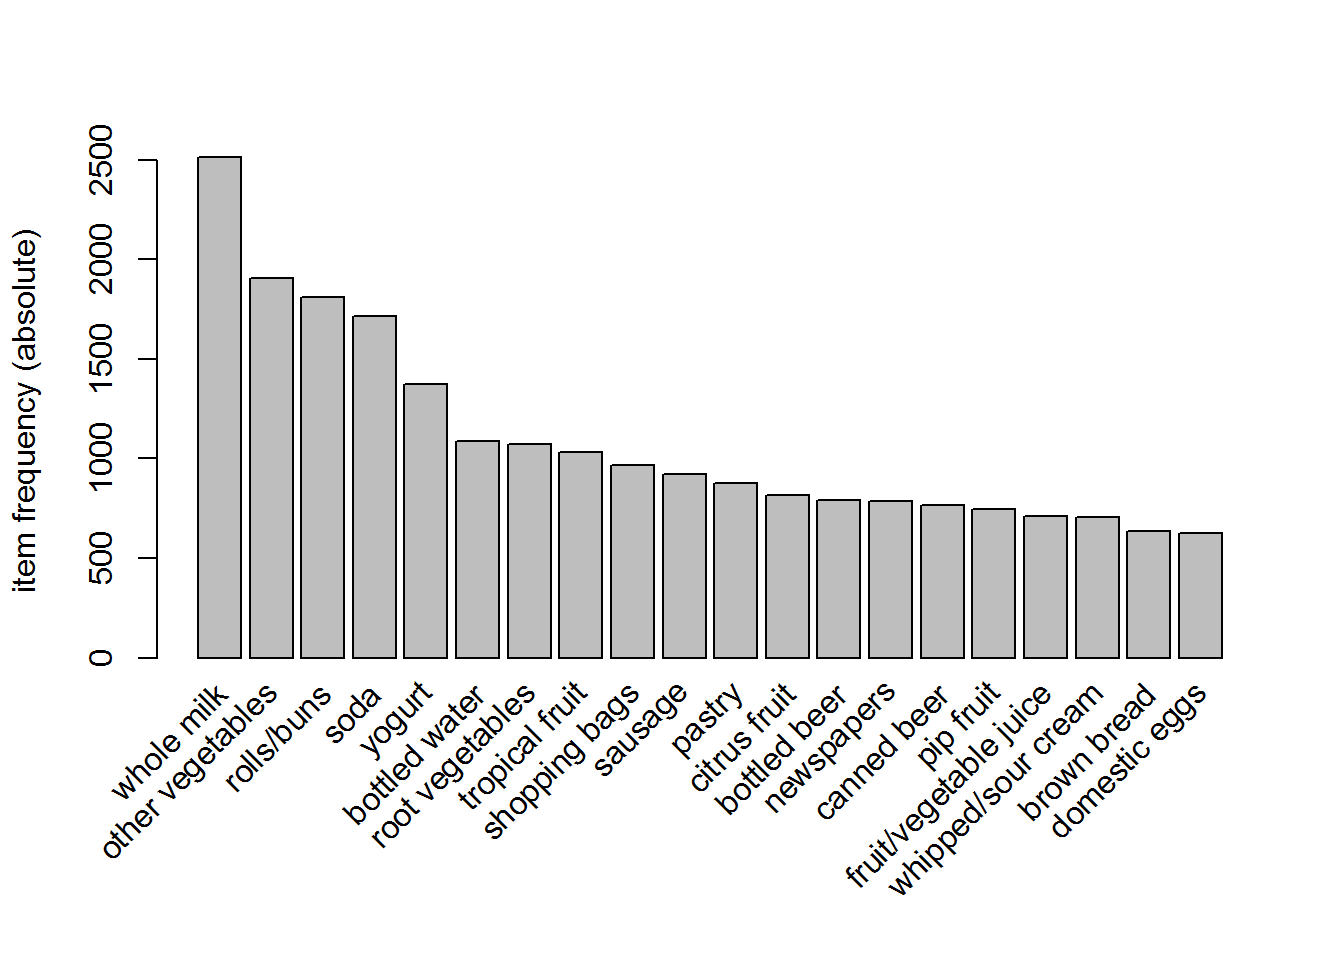
\includegraphics{bookdown_files/figure-latex/unnamed-chunk-66-1.pdf}

Như vậy, ta đã tạo xong biểu đồ water-fall đơn giản. Ở bước tiếp theo,
chúng ta cần điều chỉnh lại các thành phần cho biểu đồ.

\begin{Shaded}
\begin{Highlighting}[]
\CommentTok{# Tạo dữ liệu cho biểu đồ đường}
\NormalTok{df2 <-}\StringTok{ }\NormalTok{df }\OperatorTok\StringTok{ }\KeywordTok{select}\NormalTok{(date, eop) }\OperatorTok\StringTok{ }\KeywordTok{distinct}\NormalTok{()}

\CommentTok{# Điều chỉnh theme}
\NormalTok{p2 <-}\StringTok{ }\NormalTok{p1  }\OperatorTok{+}\StringTok{ }
\StringTok{  }\KeywordTok{geom_line}\NormalTok{(}\KeywordTok{aes}\NormalTok{(date, eop), }\DataTypeTok{col =} \StringTok{"dodgerblue4"}\NormalTok{, }\DataTypeTok{size =} \DecValTok{1}\NormalTok{) }\OperatorTok{+}
\StringTok{  }\KeywordTok{geom_point}\NormalTok{(}\KeywordTok{aes}\NormalTok{(date, eop), }\DataTypeTok{col =} \StringTok{"dodgerblue4"}\NormalTok{, }\DataTypeTok{size =} \FloatTok{2.5}\NormalTok{) }\OperatorTok{+}
\StringTok{  }\KeywordTok{geom_text}\NormalTok{(}\KeywordTok{aes}\NormalTok{(date, eop, }\DataTypeTok{label =}\NormalTok{ eop), }\DataTypeTok{vjust =} \FloatTok{1.2}\NormalTok{, }
            \DataTypeTok{hjust =} \FloatTok{-0.1}\NormalTok{) }\OperatorTok{+}
\StringTok{  }\KeywordTok{scale_fill_manual}\NormalTok{(}\DataTypeTok{values =} \KeywordTok{c}\NormalTok{(}\StringTok{"grey60"}\NormalTok{, }\StringTok{"coral2"}\NormalTok{)) }\OperatorTok{+}
\StringTok{  }\KeywordTok{theme_minimal}\NormalTok{() }\OperatorTok{+}
\StringTok{  }\KeywordTok{theme}\NormalTok{(}
    \DataTypeTok{axis.line =} \KeywordTok{element_line}\NormalTok{(}\DataTypeTok{color =} \StringTok{"gray40"}\NormalTok{, }\DataTypeTok{size =} \FloatTok{0.5}\NormalTok{),}
    \DataTypeTok{legend.position =} \StringTok{"top"}\NormalTok{) }\OperatorTok{+}
\StringTok{  }\KeywordTok{scale_x_date}\NormalTok{(}\DataTypeTok{breaks =}\NormalTok{ data}\OperatorTok{$}\NormalTok{date,}
               \DataTypeTok{date_labels =} \StringTok{"%b"}\NormalTok{) }\OperatorTok{+}
\StringTok{  }\KeywordTok{theme}\NormalTok{(}\DataTypeTok{panel.grid.minor.x =} \KeywordTok{element_blank}\NormalTok{(),}
        \DataTypeTok{legend.title =} \KeywordTok{element_blank}\NormalTok{()) }\OperatorTok{+}
\StringTok{  }\KeywordTok{ggtitle}\NormalTok{(}\StringTok{"Overview of active users"}\NormalTok{) }\OperatorTok{+}
\StringTok{  }\KeywordTok{xlab}\NormalTok{(}\StringTok{"Date"}\NormalTok{) }\OperatorTok{+}\StringTok{ }
\StringTok{  }\KeywordTok{ylab}\NormalTok{(}\StringTok{"Number of active users"}\NormalTok{)}
\NormalTok{p2}
\end{Highlighting}
\end{Shaded}

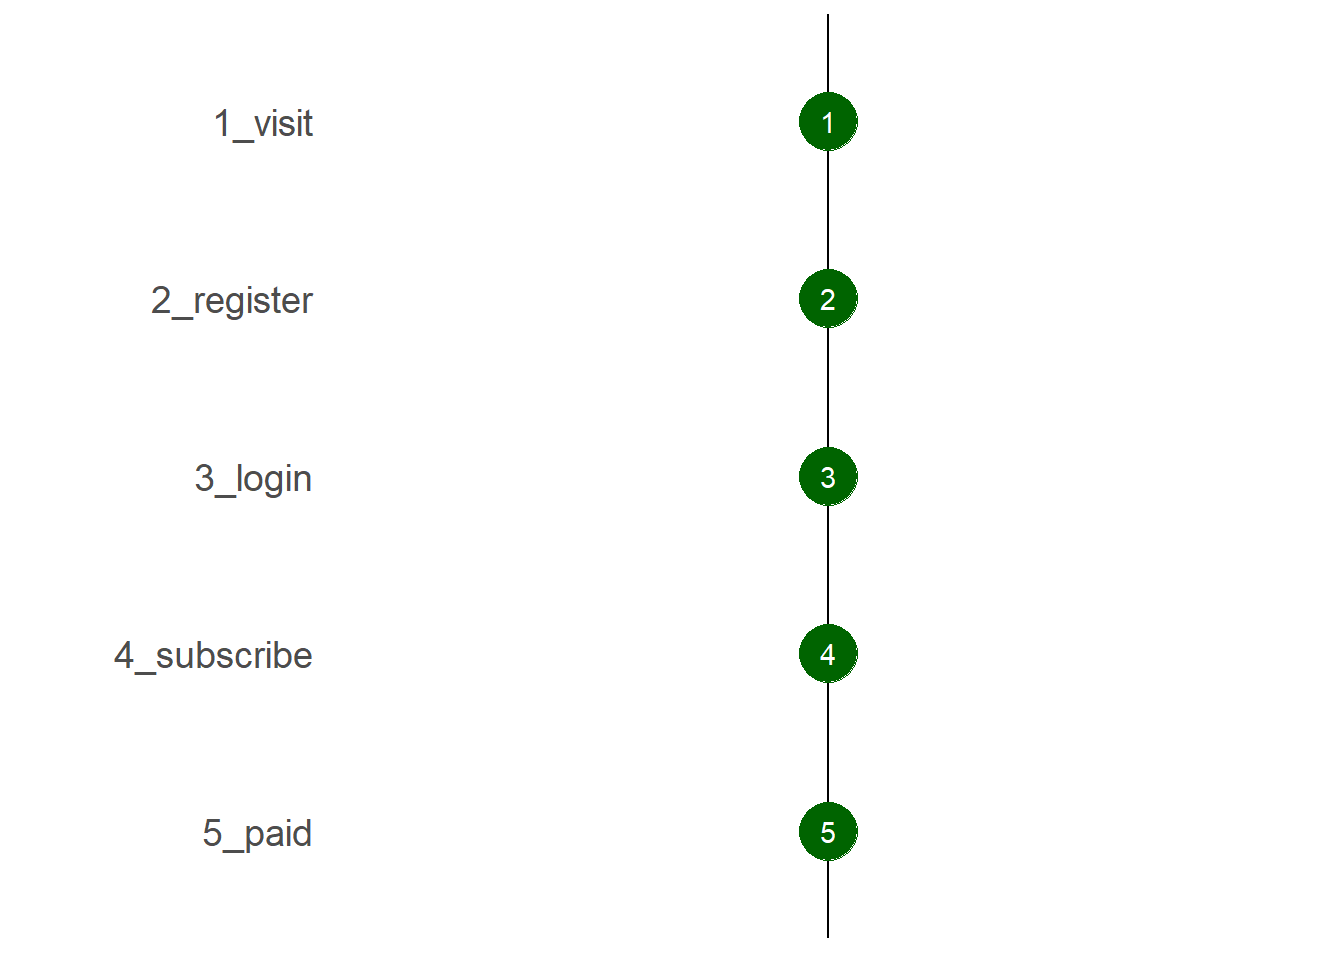
\includegraphics{bookdown_files/figure-latex/unnamed-chunk-67-1.pdf}

Bước tiếp theo, ta cần xây dựng biểu đồ bar đơn giản để có thể đưa vào
góc phần tư bên trái của biểu đồ vừa tạo.

\begin{Shaded}
\begin{Highlighting}[]
\NormalTok{p3 <-}\StringTok{ }\NormalTok{df }\OperatorTok\StringTok{ }
\StringTok{  }\KeywordTok{mutate}\NormalTok{(}\DataTypeTok{value =} \KeywordTok{case_when}\NormalTok{(}
\NormalTok{    group }\OperatorTok{==}\StringTok{ "churn"} \OperatorTok{~}\StringTok{ }\DecValTok{-1} \OperatorTok{*}\StringTok{ }\NormalTok{value,}
    \OtherTok{TRUE} \OperatorTok{~}\StringTok{ }\NormalTok{value}
\NormalTok{  )) }\OperatorTok\StringTok{ }
\StringTok{  }\KeywordTok{ggplot}\NormalTok{(}\KeywordTok{aes}\NormalTok{(date, value)) }\OperatorTok{+}
\StringTok{  }\KeywordTok{geom_bar}\NormalTok{(}\KeywordTok{aes}\NormalTok{(}\DataTypeTok{fill =}\NormalTok{ group), }\DataTypeTok{stat =} \StringTok{"identity"}\NormalTok{) }\OperatorTok{+}
\StringTok{  }\KeywordTok{scale_fill_manual}\NormalTok{(}\DataTypeTok{values =} \KeywordTok{c}\NormalTok{(}\StringTok{"grey60"}\NormalTok{, }\StringTok{"coral2"}\NormalTok{)) }\OperatorTok{+}
\StringTok{  }\KeywordTok{theme_minimal}\NormalTok{() }\OperatorTok{+}
\StringTok{  }\KeywordTok{theme}\NormalTok{(}
    \DataTypeTok{legend.position =} \StringTok{"none"}\NormalTok{,}
    \DataTypeTok{axis.title.x =} \KeywordTok{element_blank}\NormalTok{(),}
    \DataTypeTok{axis.title.y =} \KeywordTok{element_blank}\NormalTok{(),}
    \DataTypeTok{axis.ticks.y =} \KeywordTok{element_blank}\NormalTok{(),}
    \DataTypeTok{axis.text.y =} \KeywordTok{element_blank}\NormalTok{(),}
    \DataTypeTok{panel.grid.minor =} \KeywordTok{element_blank}\NormalTok{(),}
    \DataTypeTok{panel.grid.major =} \KeywordTok{element_blank}\NormalTok{(),}
    \DataTypeTok{axis.text.x =} \KeywordTok{element_text}\NormalTok{(}\DataTypeTok{angle =} \DecValTok{90}\NormalTok{)}
\NormalTok{  ) }\OperatorTok{+}
\StringTok{  }\KeywordTok{scale_x_date}\NormalTok{(}\DataTypeTok{breaks =}\NormalTok{ data}\OperatorTok{$}\NormalTok{date,}
               \DataTypeTok{date_labels =} \StringTok{"%b"}\NormalTok{) }
\NormalTok{p3}
\end{Highlighting}
\end{Shaded}

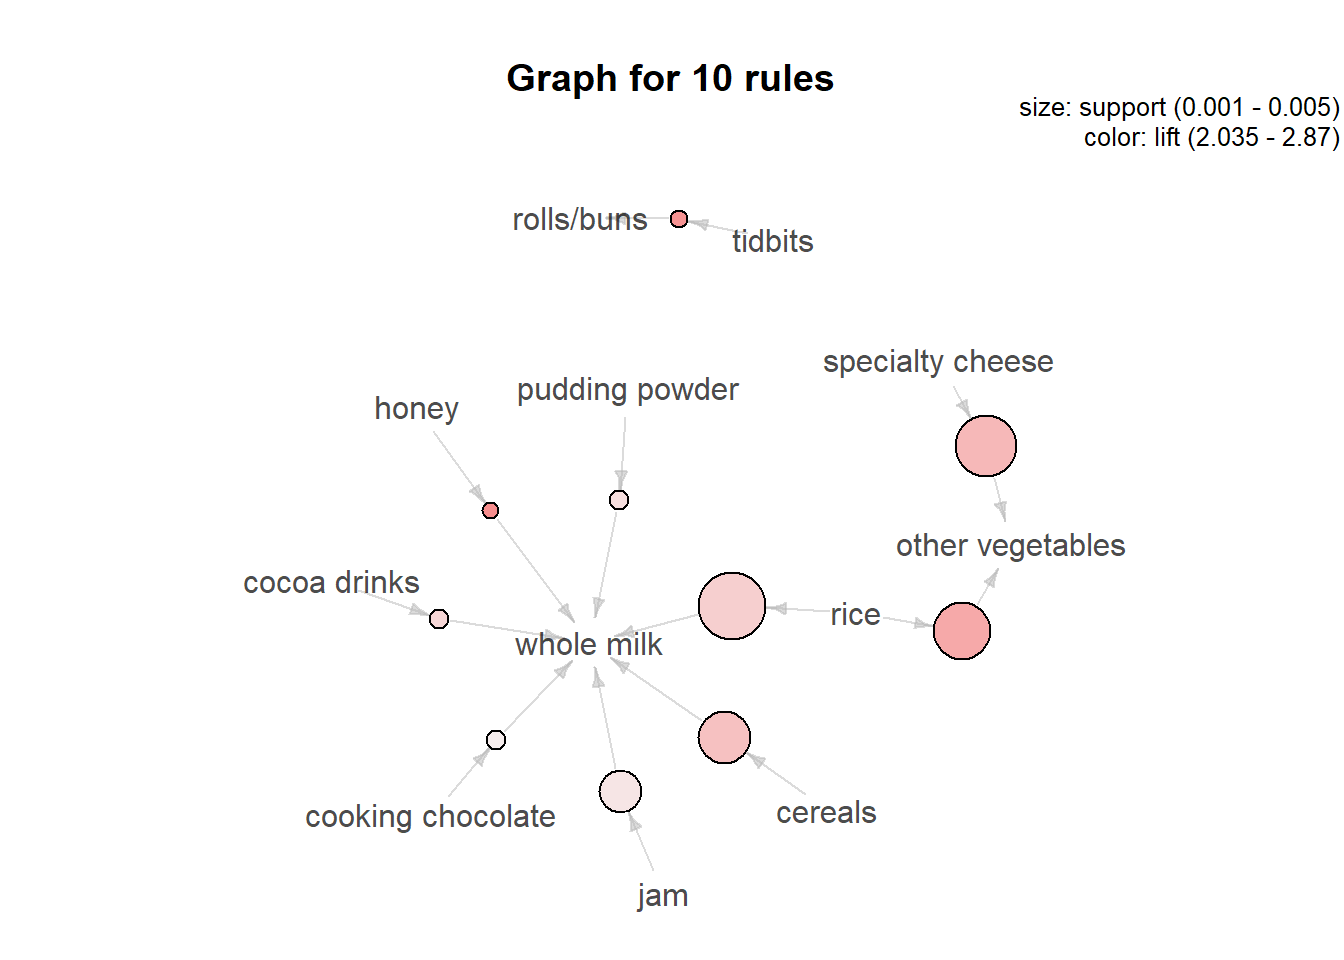
\includegraphics{bookdown_files/figure-latex/unnamed-chunk-68-1.pdf}

Cuối cùng, ta có thể nhóm hai biểu đồ trên với \texttt{grid} \&
\texttt{gridExtra}.

\begin{Shaded}
\begin{Highlighting}[]
\KeywordTok{grid.newpage}\NormalTok{()}

\CommentTok{# Xác định vị trí cho biểu đồ chính}
\NormalTok{position_}\DecValTok{1}\NormalTok{ <-}\StringTok{ }\KeywordTok{viewport}\NormalTok{(}\DataTypeTok{width =} \DecValTok{1}\NormalTok{, }\DataTypeTok{height =} \DecValTok{1}\NormalTok{, }
                       \DataTypeTok{x =} \FloatTok{0.5}\NormalTok{, }\DataTypeTok{y =} \FloatTok{0.5}\NormalTok{)  }

\CommentTok{# Vị trí cho biểu đồ phụ}
\NormalTok{position_}\DecValTok{2}\NormalTok{ <-}\StringTok{ }\KeywordTok{viewport}\NormalTok{(}\DataTypeTok{width =} \FloatTok{0.35}\NormalTok{, }\DataTypeTok{height =} \FloatTok{0.25}\NormalTok{, }
                       \DataTypeTok{x =} \FloatTok{0.25}\NormalTok{, }\DataTypeTok{y =} \FloatTok{0.75}\NormalTok{)  }

\KeywordTok{print}\NormalTok{(p2, }\DataTypeTok{vp =}\NormalTok{ position_}\DecValTok{1}\NormalTok{)}
\KeywordTok{print}\NormalTok{(p3, }\DataTypeTok{vp =}\NormalTok{ position_}\DecValTok{2}\NormalTok{)}
\end{Highlighting}
\end{Shaded}

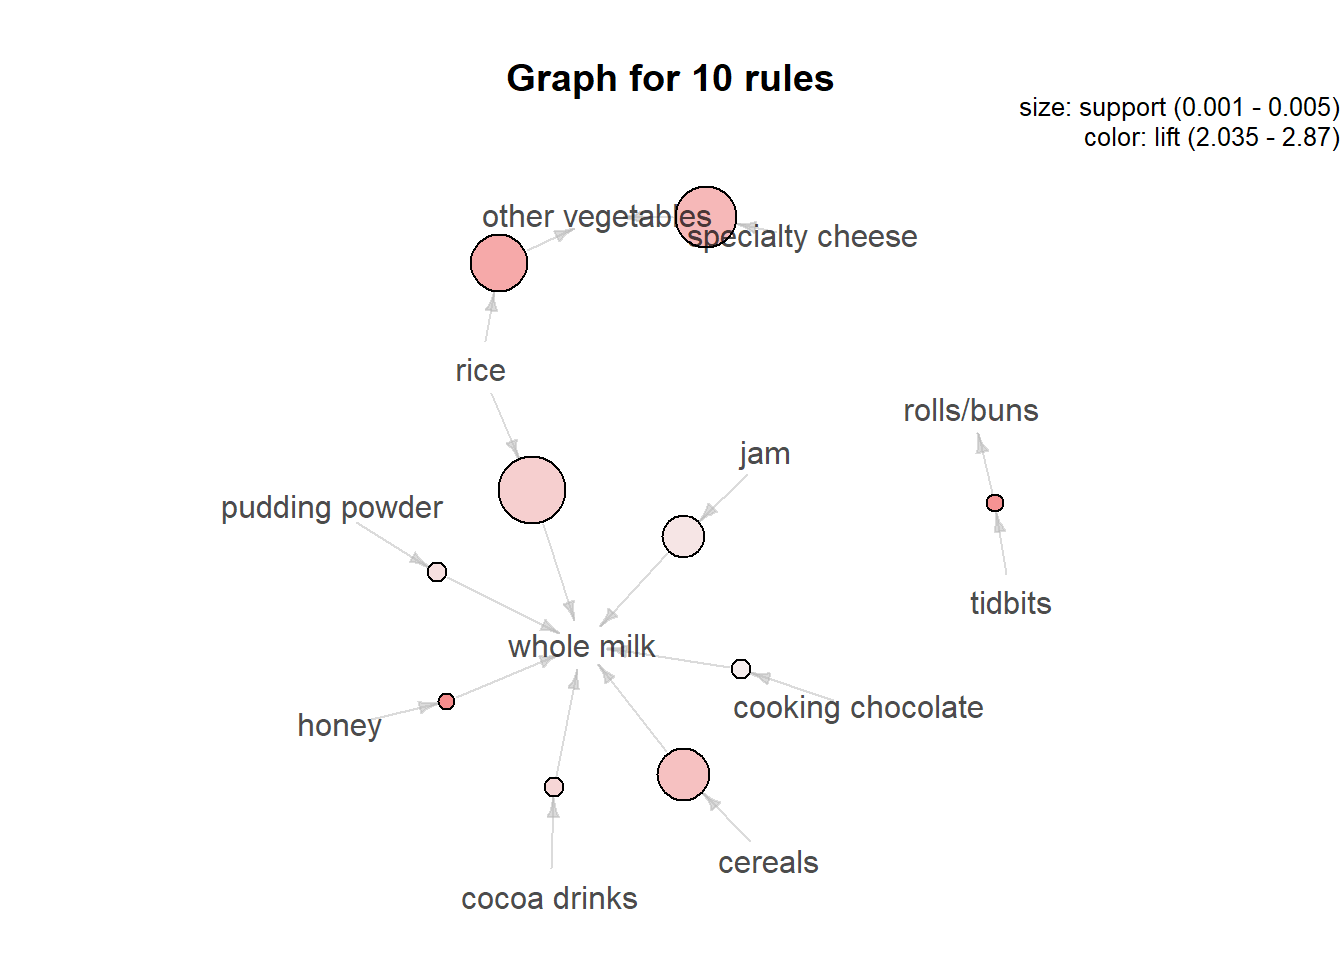
\includegraphics{bookdown_files/figure-latex/unnamed-chunk-69-1.pdf}

\cleardoublepage

\hypertarget{appendix-appendix}{%
\appendix \addcontentsline{toc}{chapter}{\appendixname}}


\hypertarget{more-to-say}{%
\chapter{More to Say}\label{more-to-say}}

Yeah! I have finished my book, but I have more to say about some topics.
Let me explain them in this appendix.

To know more about \textbf{bookdown}, see \url{https://bookdown.org}.

\bibliography{book.bib,packages.bib}

\backmatter
\printindex

\end{document}
